%!TEX program = xelatex
% 本文件由 论文.tex 自动合并生成，仅供 tex2docx / 单文件编译等用途。
% 生成时间: 2026-06-01 09:38:34
% 请勿手工编辑后反向覆盖分章草稿；请继续修改 论文.tex 与各 草稿/*.tex。
%
% HUSTthesis.tex @ https://github.com/zfengg/HUSTtex/tree/master/HUSTthesis
%
% 	A simple tex template for the undergraduate thesis at HUST.
%
% author: Zhou Feng @ 2019
%
% requirements:
%	TeX environments: TeXlive/MacTeX or MiKTeX
%	compiler: XeLaTeX
%
% ---------------------------------------------------------------------------- %
%                                   preamble                                   %
% ---------------------------------------------------------------------------- %
\documentclass[a4paper]{article}
% 10.5pt = 5 hao

% ---------------------------------- layout ---------------------------------- %
\usepackage[a4paper,top=2.5cm,bottom=2.5cm,left=3cm,right=3cm,% margins
			headheight=1.5cm,headsep=1.5em,
			footskip=2em,
			]{geometry}

% ------------------------------- math symbols ------------------------------- %
% 载入常用的数学包, 符号包
\usepackage{amsmath}
\usepackage{amsfonts}
\usepackage{amssymb}
\usepackage{mathrsfs}
\usepackage{blindtext}
% 物理量与单位格式化（4.1 节中 \SI{52.3}{mm} 等命令所需）
\usepackage{siunitx}

%----------------------------------------------------------------%
%% linespace 行间距，段间距等等
\usepackage{setspace}
% \usepackage{indentfirst} % then the first line of each title should start with a indent.
% 定义标题和段落样式
% 定义1.5倍行距
\renewcommand{\baselinestretch}{1.62}
\setlength{\baselineskip}{12pt}   % set the fixed value of the lineskip
\setlength\parskip{\baselineskip} % set the space between the paragraphs, set the variable \parskip \baselineskip
% parindent
\setlength{\parindent}{0pt}

%----------------------------------------------------------------%
% fonts (style, color, size). 字体的大小，颜色，以及定义常用的字号
\usepackage{ctex}		 	% If you are lazy, the CTEX suit is enough.
% Chinese font
\usepackage{xeCJK}		 	% For the Chinese through XeLaTex
\setCJKmainfont{FandolSong} 	% set the mainfont of Chinese as songti. (serif) for  
\setCJKsansfont{FandolSong}	% sans serif font for \textsf
\setCJKmonofont{FandolSong}	% monospace font for \texttt
% \punctstyle{kaiming}   	% Remove the space used by symbols like comma. Special for the mainland students like us HUSTers.
\setCJKfamilyfont{song}{FandolSong}                     %宋体 song
\newcommand{\song}{\CJKfamily{song}}                        
\setCJKfamilyfont{kai}{FandolKai}                        		 %楷体2312  kai
\newcommand{\kai}{\CJKfamily{kai}}  
\setCJKfamilyfont{hwzs}{FandolFang}                        %华文中宋  hwzs
\newcommand{\hwzs}{\CJKfamily{hwzs}}
\setCJKfamilyfont{hei}{FandolHei}                     %黑体  hei
\newcommand{\hei}{\CJKfamily{hei}}
% English font
\usepackage{fontspec}% Then you can use the fonts installed at your device.
\setmainfont{Times New Roman}
\setsansfont{Times New Roman}
\setmonofont{Times New Roman}
%\setsansfont{[foo.ttf]} % for the fonts at this default path.
% font Color 利用definecolor自己可以定义颜色
\usepackage{xcolor}
\definecolor{MSBlue}{rgb}{.204,.353,.541}
\definecolor{MSLightBlue}{rgb}{.31,.506,.741}
% font Size (I use pinyin represents the corresponding size in Microsorft Word)
% \newcommand{\chuhao}{\fontsize{42pt}{\baselineskip}\selectfont}
\newcommand{\xiaochuhao}{\fontsize{36pt}{\baselineskip}\selectfont}
% \newcommand{\yihao}{\fontsize{28pt}{\baselineskip}\selectfont}
\newcommand{\erhao}{\fontsize{21pt}{\baselineskip}\selectfont}
\newcommand{\xiaoerhao}{\fontsize{18pt}{\baselineskip}\selectfont}
\newcommand{\sanhao}{\fontsize{15.75pt}{\baselineskip}\selectfont}
\newcommand{\sihao}{\fontsize{14pt}{18pt}\selectfont}
\newcommand{\xiaosihao}{\fontsize{12pt}{18pt}\selectfont}
\newcommand{\wuhao}{\fontsize{10.5pt}{18pt}\selectfont}
% \newcommand{\xiaowuhao}{\fontsize{9pt}{\baselineskip}\selectfont}
% \newcommand{\liuhao}{\fontsize{7.875pt}{\baselineskip}\selectfont}
% \newcommand{\qihao}{\fontsize{5.25pt}{\baselineskip}\selectfont}

% ---------------------------------------------------------------------------- %
%% header and footer 页眉，页脚
\usepackage{fancyhdr} % for header and footer
% 设置页眉样式
\newcommand{\headstyle}{
 \fancyhead[C]{ \hwzs\wuhao 华\hspace{0.5em}中\hspace{0.5em}科\hspace{0.5em}技\hspace{0.5em}大\hspace{0.5em}学\hspace{0.5em}毕\hspace{0.5em}业\hspace{0.5em}设\hspace{0.5em}计\hspace{0.5em}(论\hspace{0.5em}文)}
}
% 设置页脚样式
\newcommand{\footstyle}{\fancyfoot[C]{\wuhao\thepage}
 \fancyfoot[L]{\rule[5pt]{6.7cm}{0.4pt}}
 \fancyfoot[R]{\rule[5pt]{6.7cm}{0.4pt}}
}
\pagestyle{fancy}
\fancyhf{} % 清空原有样式
\headstyle
\footstyle
% 定义一种新的格式叫做main
\fancypagestyle{main}{%
 \fancyhf{} % 清空原有样式
 \headstyle
 \footstyle
}
\renewcommand{\headrulewidth}{0.4pt}
% \renewcommand{\footrulewidth}{0.4pt}
% \renewcommand{\headrule}{\rule{\textwidth}{0.4pt}}

% ---------------------------------------------------------------------------- %
% set the styles of sections at all levels
% 设置各个标题样式
% 不需要使用part和chapter层级
\usepackage{titlesec}
\usepackage{titletoc}
\titleformat{\section}{\centering\hei\bfseries\xiaoerhao}{\thesection}{1em}{} % 在section标题编号后面加个点
% \titlelabel{\thetitle.\quad} % add a dot after the counter for all levels of sections
% \titleformat*{\section}{\wuhao\bfseries} % 设置标签的形式，5号加粗
\titleformat*{\subsection}{\raggedright\hei\bfseries\sihao}
\titleformat*{\subsubsection}{\raggedright\hei\bfseries\xiaosihao}
\titleformat{\paragraph}[hang]{\raggedright\hei\bfseries\xiaosihao}{\theparagraph}{1em}{}[]

% manual
% \titleformat{command}[shape]{format}{label}{sep}{before-code}[after-code]
% \titlespacing{command}{left}{before-sep}{after-sep}
% 设置新的层级subsubsubsection
\setcounter{tocdepth}{4}
\setcounter{secnumdepth}{4}

\newcommand{\sectionbreak}{\clearpage} % 小节从新的一页开始
% 根据学校要求设置新的section, subsection, subsection,  paragraph

% set the content of section and so on
\newcommand\seccontent{
	\song
	\xiaosihao % 默认五号字体, 行间距为1.5*\baselineskip
    \setlength{\parindent}{2em} % 首段缩进两个M字符
    \setlength{\parskip}{0pt}
    }
\newcommand\tabcontent{
	\song
	\wuhao % 默认五号字体, 行间距为1.5*\baselineskip
	\setlength{\parindent}{2em} % 首段缩进两个M字符
	\setlength{\parskip}{0pt}
}


% ---------------------------------------------------------------------------- %
% for the style of theorems, definitions, proofs and remarks 定义数学里面一些常用的环境
\usepackage{amsthm}
\newtheorem{thm}{\textbf{定理}}[section]
% The section in [] can be replaced by chapter or subsection
\theoremstyle{definition} 
\theoremstyle{plain}
\theoremstyle{remark}

% ---------------------------------------------------------------------------- %
% for the caption and reference 图表及公式的编号规范
\usepackage{float} 		 		  	% table figure positioning
\usepackage{caption}
\captionsetup[figure]{labelformat=default, labelsep=quad,name={图}}
\captionsetup[table]{labelformat=default,labelsep=quad,name={表}}
% 设置图表标题的计数方式
\renewcommand{\thefigure}{\ifnum \thesection>0 \thesection-\fi \arabic{figure}} % set caption label style to 2-1
\renewcommand{\thetable}{\ifnum \thesection>0 \thesection-\fi \arabic{table}} % set caption label style to 2-1
\DeclareCaptionFont{mylabelfont}{\hei\xiaosihao}
\captionsetup[figure]{font=mylabelfont}
\captionsetup[table]{font=mylabelfont}

% ----- 自定义浮动 casebox：对照样本（标准伪代码版式，ruled 上下双线）-----
% 用于 4.3.3 节两个对照用例的版面承载，与 figure/table 同级独立编号
% caption 样式：对照样本 4-1、对照样本 4-2 ...，章号自动跟随 \thesection
\floatstyle{ruled}
\newfloat{casebox}{!ht}{loc}[section]
\floatname{casebox}{对照样本}
\renewcommand{\thecasebox}{\ifnum \thesection>0 \thesection-\fi \arabic{casebox}}
\captionsetup[casebox]{labelformat=default, labelsep=quad, name={对照样本}, font=mylabelfont}
\floatstyle{plain}

% 设置图表的autoref的格式
\newcommand{\reffig}[1]{图 \ref{#1}}
\newcommand{\reftab}[1]{表 \ref{#1}}
\newcommand{\refcase}[1]{对照样本 \ref{#1}}
% 公式的编号格式
\renewcommand\theequation{\arabic{section}-\arabic{equation}}

\usepackage{graphicx} % To include graphixs 添加图所需的包
\usepackage{booktabs} % To create three line table including the commands toprule, bottomrule, and midrule
% \usepackage{colortbl} %
% 使用tabularx库并定义新的左右中格式
\usepackage{tabularx}
\usepackage{makecell}
\newcolumntype{L}{X}
\newcolumntype{C}{>{\centering \arraybackslash}X}
\newcolumntype{R}{>{\raggedright \arraybackslash}X}

% ---------------------------------------------------------------------------- %
% set the style of counters 设置计数器
% 设置重新计数的位置
\makeatletter
\@addtoreset{footnote}{page}
\@addtoreset{figure}{section}
\@addtoreset{table}{section}
\@addtoreset{equation}{section}
\makeatother

% ---------------------------------------------------------------------------- %
% tableofcontents, listoftables and listoffigures 目录
%\renewcommand\listfigurename{插图列表}
%\renewcommand\listtablename{表格列表}
%\titlecontents{标题名}[左间距]{标题格式}{标题标志}{无序号标题}{指引线与页码}[下间距]
%\dottedcontents{section}[2.55em]{\song \xiaosihao \bfseries}{2.5em}{1em}
\usepackage{tocloft}
\renewcommand{\contentsname}{\centerline{ \hei\bfseries\xiaoerhao 目\hspace{2em}录}}
\titlecontents{section}[3em]{\song\xiaosihao\bfseries}{\contentslabel{3em}}{\hspace*{-3em}}{\normalfont\titlerule*[8pt]{.}\contentspage}
\titlecontents{subsection}[3em]{\song\xiaosihao}{\contentslabel{3em}}{\hspace*{-3em}}{\titlerule*[8pt]{.}\contentspage}
\titlecontents{subsubsection}[4em]{\song\xiaosihao}{\contentslabel{4em}}{\hspace*{-4em}}{\titlerule*[8pt]{.}\contentspage}
\titlecontents{paragraph}[5em]{\song\xiaosihao}{\contentslabel{5em}}{\hspace*{-5em}}{\titlerule*[8pt]{.}\contentspage}

% ---------------------------------------------------------------------------- %
% reference and citation 参考文献
% gbt7714 (GB/T 7714-2015) 数字编号、按正文首次引用顺序编号；自带 natbib 兼容层，
% 因此 \cite{a,b,c} 仍会被自动合并为 [1-3]。
% gbt7714 在 TeX Live 2025 仍接受 numbers/sort&compress（后续版本将更名为 numerical），
% 暂保留写法不变，避免触发 natbib 选项冲突。
\usepackage[numbers,sort&compress]{gbt7714}
\renewcommand{\refname}{\centering\hei\xiaoerhao 参考文献}
\bibsep=0pt % 用来设置每个\bibitem之间的间距
% 上角标引用：直接重定义 \cite 命令，使全文所有引用都以 [\textsuperscript] 形式呈现
% （gbt7714 已设定 numerical 样式，重定义只改变上下文位置，不破坏标号顺序）
\let\oldcite\cite
\renewcommand{\cite}[1]{\textsuperscript{\oldcite{#1}}}

% ---------------------------------------------------------------------------- %
% 设置声明页
% 使用特殊符号
\usepackage{amssymb}
\usepackage{wasysym}
% 制作tatement中的符号
\def\HUSTcheckedbox{$\Square\!\!\!\!\checkmark$}
\def\HUSTbox{$\Square$}
% 设置命令
\newcommand{\statement}[2]{
	\def\yearofconfidentiality{\hspace{2em}}

    \def\HUSTconfidential{\HUSTbox}
	\def\HUSTnotconfidential{\HUSTcheckedbox}
	\ifnum #1<2
		\def\HUSTconfidential{\HUSTcheckedbox}
		\def\HUSTnotconfidential{\HUSTbox}
		\def\yearofconfidentiality{#2}
	\fi
	\clearpage
	\thispagestyle{main}
	\vspace*{1em}
	\seccontent
	\begin{center}
		\heiti \xiaoerhao \bfseries
		学位论文原创性声明
	\end{center}


    本人郑重声明：所呈交的论文是本人在导师的指导下独立进行研究所取得的研究成果。除了文中特别加以标注引用的内容外，本论文不包括任何其他个人或集体已经发表或撰写的成果作品。本人完全意识到本声明的法律后果由本人承担。

	\begin{flushright}
		作者签名：\hspace{6em} 年 \hspace{2em} 月 \hspace{2em} 日
	\end{flushright}
	\vspace{4em}

	\begin{center}
		\heiti \zihao{-2} \bfseries
		学位论文版权使用授权书
	\end{center}


    本学位论文作者完全了解学校有关保障、使用学位论文的规定，同意学校保留并向有关学位论文管理部门或机构送交论文的复印件和电子版，允许论文被查阅和借阅。本人授权省级优秀学士论文评选机构将本学位论文的全部或部分内容编入有关数据进行检索，可以采用影印、缩印或扫描等复制手段保存和汇编本学位论文。

    本学位论文属于 1、保密 \HUSTconfidential ，在 \yearofconfidentiality 年解密后适用本授权书。

		    \hspace{7em} 2、不保密 \HUSTnotconfidential \hspace{1em}
			。

			\hspace{7em} (请在以上相应方框内打``$\checkmark$'')



	\begin{flushright}
	作者签名：\hspace{6em} 年 \hspace{2em} 月 \hspace{2em} 日

    导师签名：\hspace{6em} 年 \hspace{2em} 月 \hspace{2em} 日
    \end{flushright}
	\clearpage
}
\newcommand{\makestatement}[2]{\statement{#1}{#2}}

% ---------------------------------------------------------------------------- %
% 定义中英文摘要和致谢环境
%
% 中文摘要环境
\newenvironment{cnabstract}[1]{
	\def \cnkeyword {#1}
	\clearpage
	\phantomsection
	\addcontentsline{toc}{section}{摘要}
	\vspace*{-20pt}
	\begin{center}
		\heiti \bfseries \xiaoerhao 摘 \hspace{2em} 要
	\end{center}
	\seccontent
}{
	\vspace{1em}
	\par\noindent {\hei\sihao \bfseries 关键词：} {\song\xiaosihao\cnkeyword}

}

% 英文摘要环境（局部压缩行距 + 段间距，避免长摘要把 Key Words 顶到第二页）
% 摘要拆为 3 段后内容增多，进一步把 \linespread 从 1.2 压缩到 1.1，
% 并把首段上拉量从 -30pt 增至 -40pt，把段末关键词的 \par\vspace 从 0.2em 压至 0em。
\newenvironment{enabstract}[1]{
	\def \enkeyword {#1}
	\clearpage
	\phantomsection
	\addcontentsline{toc}{section}{Abstract}
	\vspace*{-40pt}
	\begin{center}
		\bfseries \xiaoerhao Abstract
	\end{center}
	\seccontent
	\linespread{1.1}\selectfont
	\setlength{\parskip}{0pt}
}{
	\par\noindent {\xiaosihao\bfseries Key Words: }\ {\song\xiaosihao\enkeyword}
	% 末尾不再 \clearpage：\tableofcontents 内部 \section* 会触发 \sectionbreak
	% 自动 \clearpage，再次显式 \clearpage 会产生空白页。
}

% 定义致谢环境
\newenvironment{thankpage}{
	\clearpage%
	\phantomsection%
	\addcontentsline{toc}{section}{致谢}%
	\section*{致\hspace{2em}谢}%
}{
	\clearpage
}


% ---------------------------------------------------------------------------- %
%	---	定义列表项，列举的样式
\usepackage{enumitem}
\setlist{noitemsep}

% ---------------------------------------------------------------------------- %
% 中英混排断行调优
%   1. emergencystretch 给段落分行更多余量，避免长英文标识符撑出右边距。
%   2. XeTeXlinebreaklocale "zh" 允许在 CJK 字符之间任意位置分行。
%   3. \bk 是 \discretionary 的简写，用于在 \texttt{} 等不可分词内部
%      手动插入零宽允许断点（例如 \texttt{INTENT\bk\_RECOGNIZER\bk\_PROMPT}）。
\setlength{\emergencystretch}{3em}
\XeTeXlinebreaklocale "zh"
\XeTeXlinebreakskip=0pt plus 1pt
\newcommand{\bk}{\discretionary{}{}{}}

% ---------------------------------------------------------------------------- %
% \usepackage{makeindex} For the index 索引
\usepackage{listings} % For the code. 代码

% ---------------------------------------------------------------------------- %
% 设置脚注

% ---------------------------------------------------------------------------- %
%% For the hyperlink and bookmark 超链接及书签，(这样生成的pdf中的引用直接点击链接即可到达目的地)
\usepackage[bookmarks=true,colorlinks,linkcolor=black,citecolor=black,urlcolor=purple]{hyperref}% 设置超链接并修改风格


% ---------------------------------------------------------------------------- %
%% For the appendix, 附录
% 设置附录
\usepackage{appendix}
\renewcommand{\appendixname}{附录}

% ---------------------------------------------------------------------------- %
% for the titlepage 标题页，此处可以省略，建议直接使用官方给出的标题页即可
\usepackage{titling}
% 重置命令 maketitle
\renewcommand{\maketitle}{
	\def\HUSTtitlelength{12em}
 	\begin{titlepage}
		\begin{center}
			\vspace*{0em}
			\includegraphics[height=1.61cm]{HUSTlogo.eps}\\
%
			\vspace*{4em}
%
			{\xiaochuhao \hwzs \bfseries 本科生毕业设计[论文]}\\
%
			\vspace*{6em}
			{\erhao \hei \bfseries \thetitle}

			\vspace*{6em}
			{\sanhao \hwzs
				\renewcommand\arraystretch{2.7}
				\begin{tabular}{lc}
					\makebox[4em][s]{院 \hfill 系} &
					\underline{\makebox[\HUSTtitlelength]{\school}} \\
					\makebox[4em][s]{专业班级} &
					\underline{\makebox[\HUSTtitlelength]{\classnum}} \\
					\makebox[4em][s]{姓 \hfill 名} &
					\underline{\makebox[\HUSTtitlelength]{\theauthor}} \\
					\makebox[4em][s]{学 \hfill 号} &
					\underline{\makebox[\HUSTtitlelength]{\stunum}} \\
					\makebox[4em][s]{指导教师} &
					\underline{\makebox[\HUSTtitlelength]{\instructor}} \\
			  \end{tabular}
		    }

			\vspace{4em}
			{\sanhao \hwzs \thedate}

		\end{center}
	\end{titlepage}
}

% ------------------------------------ 标题页 ----------------------------------- %
\title{毕业论文题目} % 论文题目
\def\school{数学与统计学院} % 院系
\def\classnum{专业班级} % 专业班级
\author{学生姓名} % 姓名
\def\stunum{U201512345}	% 学号
\def\instructor{导师姓名} % 指导老师
\date{\today} % 日期

% -------------------------------- quickinput -------------------------------- %
% 利用\newcommand{cmd}{def} 设置一些常用的代码，提高效率，这里可以自行删除，下面是我敲翻译时候打的一些command。
\newcommand{\hongzifuzhu}[1]{\textcolor{red}{\kai \wuhao(#1)}}

% ---------------------------------------------------------------------------- %
%                                   document                                   %
% ---------------------------------------------------------------------------- %
\begin{document}

% \maketitle  % TODO: 调用需要 HUSTlogo.eps，从 https://github.com/zfengg/HUSTtex 仓库下载后取消注释。当前为方便草稿编译先暂时注释。

% \thispagestyle{empty}% 标题页不参与编号
% ------------------------------------ 声明页 ----------------------------------- %
\setcounter{page}{1}
\renewcommand{\thepage}{\Roman{page}}
\makestatement{2}{2019} % 生成声明页, 第一个参数选择1则加上保密的时间，此处为2019，如果选择2则选择不保密。

% ----------------------------------- 中文摘要 ----------------------------------- %
\setcounter{page}{1}
\renewcommand{\thepage}{\Roman{page}}
\begin{cnabstract}{大语言模型；智能体；ReAct 范式；检索增强生成；语义桥接；幻觉抑制}
	\hspace{2em}气象预报数据是支撑国民经济与社会发展的重要基础信息资源，其获取
	与分析当前面临两类深层次技术鸿沟，一类来自不同机构与平台的接口、字段、错误
	码体系不一致带来的数据异构性，另一类来自数值数据到自然语言决策语义之间的
	认知差距。与此同时，以大语言模型为推理核心的智能体在数值边界判定、统计计算
	与权威引用等任务上存在内在的幻觉边界，直接将其应用于气象预报数据分析会引发
	引用编造、分级编造、数值漂移等严重的可信度问题。

	本文基于 ReAct 范式设计并实现了一个面向气象预报数据检索与
	分析的单智能体系统，把课题归纳为气象任务指令解析、气象数据异构特征、大语言
	模型数值与逻辑幻觉三个研究问题，并据此提出与落地了五项特色工作，分别为基于
	工具学习的异构 API 统一封装、意图识别加参数补全的双阶段自然语言理解管线、
	混合检索与确定性分级器构成的双通路 RAG 架构、基于代码生成与受限沙箱的
	确定性统计分析机制，以及覆盖模块层与集成层的多层评测体系。

	本文完成了由 5 套独立评测集共 214 条用例构成的系统化实证。
	意图识别端到端通过率 91.4\%，多地点角色识别准确率 100\%；通路 A 混合检索
	Top-1 命中率 85.0\%、MRR 0.908；通路 B 桥接的等级编号准确率与权威标准
	引用真实性同时达到 100\%，与大语言模型自由发挥的基线在严格命中率上形成
	74.6 个百分点差距；代码执行档数值准确率比大语言模型自由直算高出 22.2 个
	百分点；端到端集成评测中 \texttt{full} 档对 \texttt{ablated} 去 RAG 对照
	档的通过率高出 13.4 个百分点，权威引用率高出 26.7 个百分点，
	\texttt{decision\_support} 类用例通过率高出 50 个百分点。实证结果系统
	验证了所提架构在气象预报数据智能检索与分析任务上的有效性，同时揭示了从
	模块层到集成层的衰减效应，为后续研究指明了显式对话状态跟踪、知识库扩展、
	安全沙箱升级等具体方向。
\end{cnabstract}

% ----------------------------------- 英文摘要 ----------------------------------- %
\begin{enabstract}{Large Language Model; Agent; ReAct Paradigm; Retrieval-Augmented Generation; Semantic Bridging; Hallucination Mitigation}

	Weather forecast data is a critical information resource for the
	national economy and social development, but its acquisition and analysis
	currently face two fundamental technical gaps. One stems from data
	heterogeneity across providers in terms of interfaces, field names and error
	code conventions, while the other arises from the cognitive gap between
	numerical data and natural-language decision semantics. Meanwhile, large
	language model based agents exhibit inherent hallucination boundaries on
	numerical thresholding, statistical computation and authoritative citation,
	so directly applying them to weather forecast data analysis raises serious
	credibility concerns including citation fabrication, grade fabrication and
	numerical drift.

	This thesis designs and implements a single-agent system for
	weather forecast data retrieval and analysis based on the ReAct paradigm. The
	research is decomposed into three specific questions, namely instruction
	parsing of weather tasks, heterogeneity handling of weather data, and
	numerical and logical hallucination of large language models. Five innovations
	are proposed accordingly, including unified encapsulation of heterogeneous
	APIs based on tool learning, a two-stage natural language understanding
	pipeline combining intent recognition and parameter completion, a dual-path
	RAG architecture composed of hybrid retrieval and deterministic classifiers,
	a deterministic statistical analysis mechanism based on code generation and
	a sandboxed executor, and a multi-layer evaluation system covering both
	module-level and integration-level perspectives.

	A systematic empirical study is conducted on five independent
	benchmarks with a total of 214 test cases. Intent recognition reaches an
	end-to-end pass rate of 91.4\% with 100\% accuracy on multi-location role
	identification. Path A hybrid retrieval achieves a Top-1 hit rate of 85.0\%
	and MRR of 0.908. Path B bridging attains 100\% accuracy on grade identifiers
	and 100\% citation authenticity, with a 74.6 percentage-point gap on strict
	citation hit rate over the free-generation LLM baseline. Code execution
	improves numerical accuracy by 22.2 percentage points compared to direct LLM
	calculation. In the end-to-end evaluation, the \texttt{full} configuration
	outperforms the \texttt{ablated} non-RAG baseline by 13.4 percentage points
	in overall pass rate, 26.7 percentage points in authoritative citation rate,
	and 50 percentage points on the \texttt{decision\_support} category. The
	results validate the effectiveness of the proposed architecture for
	intelligent weather forecast data retrieval and analysis, and reveal an
	integration decay effect from module-level to integration-level evaluation,
	pointing to future directions including explicit dialogue state tracking,
	knowledge base expansion, and sandbox security upgrade.
\end{enabstract}


\vspace*{-1em}
% 2026-05-07 修复：原 TOC 因默认节间距较大加上 6 个 section + 25+ subsection
% 共 37 条条目，单页放不下导致 6.3 / 致谢 / 参考文献 / 附录 4 条目录条目
% 被挤出页脚后被紧随的 \clearpage 截断。
% 修复方案：① 不再用 \begingroup ... \endgroup 包裹 \tableofcontents，
% 因为 group 与 toc 跨页 \write 机制冲突会让 toc 第二页丢失；② 直接全局
% 压紧 tocloft 节间距（\cftbeforesecskip 0pt + \cftbeforesubsecskip -0.1em
% 负值进一步收紧 subsection 行）；③ 用 \linespread{0.92}\selectfont 微压
% 行距 8%。三档压缩共节省约 290pt 高度，让 37 条条目稳定单页收纳，且不需要
% \enlargethispage 兜底（后者会把英文摘要末段内容拉到目录页顶）。
% 注意 tocloft 寄存器名是简写 \cftbeforesecskip 而非 sectionskip。
% 2026-05-15 调整：原参数过紧使目录堆在页面中央留大段空白；放松到刚好
% 占满一页且不溢出。\linespread 1.0、\cftbeforesecskip 0.25em（章前留呼吸）、
% \cftbeforesubsecskip 0pt（子节恢复默认）。如未来章节增减导致溢出，应优先
% 回收 \cftbeforesecskip 至 0.15em，再考虑回压 \linespread 到 0.96。
\setlength{\parskip}{0pt}
% 关键发现：\cftbeforesecskip / \cftbeforesubsecskip 在当前 article + tocloft 环境下
% 被全局压制（0.65em → 1.5em 实测末项 yMax 仅变化 1.2pt）；真正能拉开间距的是
% \linespread。33 条 toc 项每行 ≈ 14pt，放大到 1.15 倍 → 每行 +2.1pt，共 +69pt
% 足以填满 46pt 顶/底空隙，留 23pt 安全余量。
\setlength{\cftbeforesecskip}{0.4em}
\setlength{\cftbeforesubsecskip}{0.05em}
{\linespread{1.07}\selectfont
\tableofcontents
\par}
\thispagestyle{main}


\clearpage
\setcounter{page}{1}
\renewcommand{\thepage}{\arabic{page}}

% ----------------------------------- 主体内容 ----------------------------------- %
% ============================================================ %
% 第 1 章：绪论
%   - 1.1 研究背景与意义
%   - 1.2 国内外研究现状（气象 AI / Agent 技术 / RAG 与工具学习 / 课题定位）
%   - 1.3 主要研究内容（研究内容与论文结构 / 研究方法与技术路线 / 论文特色）
%
% 注：原 1.4 论文组织结构已合并进 1.3.1 研究内容与论文结构，
%     1_4_论文组织结构.tex 仅作为历史素材保留，不再 \input。
% ============================================================ %
\seccontent
\section{绪论}
\label{chap:introduction}

% ===== BEGIN: 草稿/1_1_研究背景与意义 =====
% =============================================================================
% 1.1 研究背景与意义
% 草稿版本：v0.1 (2026-05-05)
% 字数：约 1500 字
% 风格规则：v0.2 风格（无 \textbf / \textit / 引例括号 / 双引号 / 破折号）
% 引用：\cite{ref2, ref5, ref10, ref18, ref25}
% 依赖宏包：booktabs / tabularx（主稿已加载）
% =============================================================================

\subsection{研究背景与意义}
\label{sec:background}

气象预报数据是支撑国民经济与社会发展的重要基础信息资源。随着全球
气候变化加剧，极端天气事件的发生频率与强度持续攀升，精准获取与
深度分析气象预报信息已成为防灾减灾、农业生产、能源调度、交通运输
等众多领域的迫切需求 \cite{ref2, ref5}。据中国气象局公布的统计
数据，我国每年因气象灾害造成的直接经济损失占国内生产总值的 1\%
至 3\%，气象服务的精准化与智能化对降低灾害损失具有现实意义。

然而，当前气象预报数据的获取与分析面临两类深层次技术鸿沟，一类
来自数据接入侧的接口异构性，另一类来自数据解读侧的认知差距，二
者在不同环节同时阻碍着气象数据的智能化利用。

数据接入侧的异构性鸿沟体现为多源数据规范的不统一。气象数据来源
于中国气象局、欧洲中期天气预报中心、美国国家海洋和大气管理局
以及和风天气、Open-Meteo 等多种公开商业平台，不同来源的观测
数据、数值预报产品、卫星遥感资料在数据格式、时空分辨率、要素
类型上差异巨大 \cite{ref25}。专业用户需同时掌握多种 API 接口
规范、字段命名约定与错误码体系才能完成跨平台的数据检索。例如
和风天气以 \texttt{LocationID} 作为地点标识符并以 \texttt{code}
字段返回状态码，而 Open-Meteo 直接以经度纬度作为参数并以
\texttt{error} 字段返回错误描述。这种接口层异构性对终端用户构成
了显著的工程门槛。

数据解读侧的语义鸿沟体现为数值表达与决策语义之间的形态错位。气象
数据以高度结构化的数值形式存在，例如 24 小时累积降水量为
\SI{52.3}{mm}、10 米高度风速为 $\SI{14.1}{m/s}$，而决策语义却以
自然语言形式表达，例如暴雨预警、不宜户外作业、建议携带雨具。
普通用户难以从大量原始数值中提炼出具有决策参考价值的判断。这一从
数值数据到决策语义的认知鸿沟使得气象预报数据的潜在价值未能被
充分释放。

与此同时，以大语言模型为核心的 AI 智能体技术正在迅速发展。Xi 等
\cite{ref10} 在综述中系统梳理了基于大语言模型的智能体在感知、推理、
规划、工具使用等方面的能力框架。Yao 等 \cite{ref18} 提出的 ReAct
范式让大语言模型能够在推理过程中与外部工具交互执行动作，为将大
语言模型应用于需要外部数据获取与计算的实际任务提供了可行路径。
李特等 \cite{ref2} 与代刊等 \cite{ref5} 分别探讨了 AI 智能体与
大语言模型在天气预报业务中的应用前景，指出利用大语言模型的自然
语言理解与推理能力来桥接用户需求与气象数据之间的鸿沟，是气象
信息服务智能化的重要方向。

基于上述背景，本文针对气象数据接入侧的异构性问题与数据解读侧的
语义鸿沟问题，设计并实现一个基于 AI 智能体的气象预报数据检索与
分析系统。系统以大语言模型为推理引擎，采用 ReAct 范式构建单
智能体架构，通过工具学习自动调用气象 API 完成数据检索，并融合
代码生成与语义桥接机制实现确定性的统计分析与自适应的报告生成。
本文研究意义可从工程实践、方法论沉淀与评测体系三个层面归纳。

在工程实践层面，本文为面向终端用户的气象信息服务智能化提供了一
套从自然语言查询到决策报告的完整技术链路，把原本需要专业人员
逐步操作的多源 API 调用、数据筛选、统计计算、术语解读、规范引用
等繁琐工作一次性自动化，把气象数据获取的工程门槛从 API 编程
水平降低到自然语言对话水平。

在方法论沉淀层面，本文提出的双通路 RAG 架构与代码生成加受限沙箱
方案在气象领域系统化地解决了大语言模型的数值与引用幻觉问题。
该方法论的核心思路是把高风险任务从大语言模型内部转移到外部确定
性组件，让大语言模型只承担擅长的语言组织职责，避免在数值边界、
权威引用、统计计算等模型不擅长的环节强行使用其内部知识。这一
思路在其他垂直领域的智能体设计中具有可迁移性。

在评测体系层面，本文构建了 5 套覆盖意图识别、检索、桥接、代码
执行、端到端共 214 条用例的多层评测体系，并在系统开发过程中
完成了 3 次知识库的人工核对与 24 处错误修正。该评测过程为本文
所设计方法在意图识别、语义桥接等关键环节的工程可靠性提供了
可复现的量化记录，所产生的评测集与核对表也可作为后续相关研究的
对照基线。

本章后续内容首先综述与本课题密切相关的国内外研究进展，进而阐述
本文的研究内容、研究方法与论文特色，最后给出全文的组织结构。

% ===== END: 草稿/1_1_研究背景与意义 =====


% ===== BEGIN: 草稿/1_2_国内外研究现状 =====
% =============================================================================
% 1.2 国内外研究现状
% 草稿版本：v0.1 (2026-05-05)
% 字数：约 2200 字
% 风格规则：v0.2 风格（无 \textbf / \textit / 引例括号 / 双引号 / 破折号）
% 引用：\cite{ref1, ref2, ref5, ref6, ref7, ref8, ref9, ref10, ref11, ref12,
%        ref13, ref15, ref16, ref17, ref18, ref19, ref20, ref21, ref22, ref23,
%        ref24, ref25, ref26, ref27, ref28, ref29, ref30}
% 依赖宏包：booktabs / tabularx（主稿已加载）
% =============================================================================

\subsection{国内外研究现状}
\label{sec:related-work}

本课题涉及的研究方向主要包括气象预报领域的 AI 应用、基于大语言
模型的 AI 智能体技术、检索增强生成与工具学习三个方向。本节按
这三个方向分别综述其研究现状与发展趋势，并在最后归纳现有研究
的不足以及本课题的定位。

\subsubsection*{1.2.1 \quad 气象预报领域的 AI 应用}

近年来深度学习在气象预报领域取得了突破性进展。华为公司的盘古
气象大模型 \cite{ref16} 首次实现了基于三维神经网络的中期全球
天气预报，在多项气象要素的预报精度上达到甚至超越欧洲中期天气
预报中心的传统数值预报模型。Google DeepMind 的 GraphCast
\cite{ref17} 通过图神经网络在 10 天全球天气预报任务上展现出
卓越性能。国内的风乌 \cite{ref26} 与伏羲 \cite{ref27} 模型分别
在中期预报精度与长时效级联预报方向取得重要进展。盛杰等 \cite{ref7}
对临近气象预报大模型风雷的 V1 版本进行了系统检验评估。李怡然等
\cite{ref6} 提出了基于气象大模型的门控时空融合网络闪电预报方法。
彭跃华等 \cite{ref8} 探索了盘古气象大模型与控制论的融合用于
台风预测分析。Rasp 等 \cite{ref25} 建立的 WeatherBench 2 为数据
驱动的气象模型提供了标准化评测基准。

上述工作主要聚焦于预报精度的提升，回答了如何预报得更准这一问题,
但较少关注预报数据的智能检索与分析，即如何让用户更便捷地获取并
理解预报信息。代刊等 \cite{ref5} 指出，大语言模型在天气预报中的
应用不应局限于预报本身，还应拓展到预报解释、数据检索、报告生成
等业务辅助环节。李特等 \cite{ref2} 进一步提出了 AI 智能体在天气
预报业务中的应用框架构想，强调智能体在异构数据访问、多步骤任务
执行、人机交互三方面的独特优势。陈敏等 \cite{ref9} 在强对流天气
预测的深度学习综述中也表明，气象领域的深度学习应用正向更加智能
化的方向演进。Kim 等 \cite{ref1} 提出的 CLIMATEAGENT 系统进一步
证实了多智能体编排在复杂气象数据科学工作流中的可行性，但其架构
偏向多智能体协作的科研工作流场景，与面向终端用户的轻量化检索
分析需求存在差异。

\subsubsection*{1.2.2 \quad 基于大语言模型的 AI 智能体技术}

AI 智能体是指具备自主感知环境、制定计划、执行行动能力的智能
系统。Xi 等 \cite{ref10} 在综述中系统归纳了基于大语言模型的
智能体的核心能力框架，包含配置 (Profile)、记忆 (Memory)、
规划 (Planning)、行动 (Action) 四个维度。

在推理与规划方向，Wei 等 \cite{ref13} 提出的思维链 (Chain-of-Thought,
CoT) 提示方法显著提升了大语言模型的复杂推理能力，让模型在算术、
常识推理、符号操作任务上的表现接近人类专家水平。Yao 等 \cite{ref30}
提出的思维树 (Tree of Thoughts, ToT) 进一步把推理过程拓展为
树状搜索结构，增强了大语言模型解决需要多步规划问题的能力。最具
影响力的是 Yao 等 \cite{ref18} 提出的 ReAct 范式，该范式把推理
与行动统一在交替循环的框架中：模型先生成思考来分析当前状态，再
决定执行一个动作调用外部工具，最后根据观察到的结果进行下一步
推理。这一范式为构建能够与外部环境交互的智能体提供了基础架构。

在工程框架方向，LangChain \cite{ref15} 提供了构建大语言模型应用
与 Agent 的成熟组件库，支持工具编排、记忆管理与多种 Agent 范式,
是当前应用最广的 Agent 开发框架。Wu 等 \cite{ref19} 提出的
AutoGen 面向多智能体协作场景，让多个具有不同角色的 Agent 通过
结构化对话协作完成复杂任务。Hong 等 \cite{ref20} 的 Data Interpreter
专门面向数据科学任务，通过大语言模型生成并执行代码来完成数据
分析，为解决大语言模型数值计算幻觉问题提供了重要参考。Boiko 等
\cite{ref23} 在自主化学研究中的成功实践展示了大语言模型 Agent
在科学研究领域的潜力。Qian 等 \cite{ref29} 的 ChatDev 工作展示了
通过多智能体协作生成代码的能力，为代码生成驱动的数据分析方案
提供了思路。

\subsubsection*{1.2.3 \quad 检索增强生成与工具学习}

检索增强生成是解决大语言模型知识局限性的核心技术路线。Lewis 等
\cite{ref12} 首次提出 RAG 框架，通过在生成过程中动态检索外部
知识库来增强大语言模型的输出质量。Gao 等 \cite{ref24} 的综述
全面梳理了 RAG 在大语言模型时代的最新进展，涵盖检索策略优化、
知识库构建、端到端训练等方向。黄冰 \cite{ref4} 在古生物学领域
的 RAG 知识问答系统实践表明，RAG 技术能够有效地把领域专业知识
注入到大语言模型中，提升垂直领域的问答准确率。

工具学习是 AI 智能体执行外部操作的关键能力。Schick 等 \cite{ref21}
的 Toolformer 让语言模型学会自主调用计算器、搜索引擎等外部工具,
开创了大语言模型主动使用工具的研究方向。Patil 等 \cite{ref28}
的 Gorilla 专注于大语言模型与大规模 API 的连接，通过检索感知
训练显著提升了 API 调用的准确性。Model Context Protocol
\cite{ref11} 作为新兴的工具协议标准，为智能体与外部工具及数据
源的标准化交互提供了统一规范。林怡等 \cite{ref3} 在 RESTful API
识别方面的工作也为 API 工具封装提供了方法论参考。Gruver 等
\cite{ref22} 的研究表明大语言模型具备零样本时间序列预测能力，
但同时揭示了其在精确数值计算方面的局限性，与 Hong 等 \cite{ref20}
观察到的代码生成必要性形成了相互印证。

\subsubsection*{1.2.4 \quad 现有研究的不足与本课题的定位}

综合上述综述可以归纳出现有研究三方面的不足。

第一是气象 AI 研究偏重预报建模而忽视数据检索与分析的智能化。
现有气象 AI 工作大多致力于提升预报精度，盘古、GraphCast、风乌、
伏羲等大模型 \cite{ref16, ref17, ref26, ref27} 都聚焦于网格化
气象要素的预测精度提升，却缺少面向终端用户的智能数据检索与分析
系统。这导致预报模型产出的高精度数据与终端用户能感知到的决策
价值之间始终存在转化缺口。

第二是通用 Agent 框架缺乏气象领域适配。现有大语言模型 Agent
框架例如 LangChain \cite{ref15} 与 AutoGen \cite{ref19} 虽然
提供了通用的工具调用与多 Agent 协作能力，但未针对气象数据的
异构性、气象术语的专业性、气象分析任务的特殊性进行优化。Kim 等
\cite{ref1} 的 CLIMATEAGENT 是少有的气象领域专门 Agent 工作,
但其多智能体协作架构与面向终端用户的轻量化检索分析需求在工程
形态上存在显著差异。

第三是大语言模型在数值分析中的幻觉问题尚未在气象场景中得到
系统解决。Hong 等 \cite{ref20} 与 Gruver 等 \cite{ref22} 的工作
共同揭示了大语言模型在数值计算与时间序列分析中存在的幻觉，
Data Interpreter \cite{ref20} 提出了通用的代码生成方案，但
气象场景下的数值理解还涉及国家标准引用、分级阈值归属、跨要素
组合判定等更细致的语义层面，需要在通用代码生成方案之上叠加领域
特定的语义桥接机制。如何在气象数据统计分析的具体场景中设计可靠
的确定性计算与权威引用机制，仍缺乏系统性研究。

本课题针对上述三方面不足，提出基于 ReAct 范式的气象 AI 智能体
方案，融合工具学习、RAG 知识注入、代码生成驱动的确定性分析、
语义桥接机制四类技术，构建从自然语言查询到气象决策报告的完整
技术链路。具体研究内容与特色工作在 \ref{sec:research-content}
节展开。

% ===== END: 草稿/1_2_国内外研究现状 =====


% ===== BEGIN: 草稿/1_3_主要研究内容 =====
% =============================================================================
% 1.3 主要研究内容
% 草稿版本：v0.3 (2026-05-07)
%   v0.1：三个研究问题 + 五项特色工作 + 研究方法。
%   v0.2：按导师意见 4 重构为"研究内容与论文结构 / 研究方法与技术路线 /
%         论文特色"三个小节；新增原理图（论文结构图 / 研究技术路线图）。
%   v0.3：按导师反馈删除研究路线图（fig:research-roadmap）以避免与论文
%         结构图、研究技术路线图存在功能重叠；研究阶段叙述改为纯文字。
% 字数：约 2200 字
% 引用：\cite{ref13, ref18, ref12, ref21, ref28}
% 图表：
%   - 图 \reffig{fig:thesis-structure}     论文结构图
%   - 图 \reffig{fig:tech-roadmap}         研究技术路线图
%   - 表 \reftab{tab:contributions}        五项特色工作概览
% 依赖宏包：booktabs / tabularx / graphicx（主稿已加载）
% =============================================================================

\subsection{主要研究内容}
\label{sec:research-content}

针对前节归纳出的三方面研究不足，本文围绕基于 AI 智能体的气象预报数据
检索与分析这一总体目标，从研究内容、研究方法与论文特色三个层面对所
提方案进行整体定位。

\subsubsection*{1.3.1 \quad 研究内容与论文结构}

本文研究内容收敛为三个相互独立又相互衔接的核心研究问题。

第一个核心研究问题是气象任务指令解析问题。该问题关注用户自然语言查询
到结构化检索意图与可执行 API 调用参数之间的精确映射，涉及命名实体
识别、相对时间消歧、参数枚举映射、缺失参数推理与对抗鲁棒性五类子任务。

第二个核心研究问题是气象数据的异构特征分析问题。该问题关注多源气象
数据在数据源、数据粒度、数据要素三个层面的差异，要求在不损失原始
数据精度的前提下把多源数据统一为大语言模型可消费的标准接口与语义化
语料，是气象 Agent 中段流水线必须解决的关键问题。

第三个核心研究问题是大语言模型在数值计算与逻辑推理中的幻觉问题。该
问题关注气象数据的统计分析与决策报告生成对数值精度与权威引用的严格
要求，要求通过架构层面的设计避免大语言模型在数值边界判定、统计计算、
标准引用等高风险任务上的失败。

为系统呈现上述三个研究问题在各章中的承接关系，本文按问题分析、方法
实现、实验验证三段式逻辑组织全文，共划分为五章主体内容加一章总结展
望，整体结构如 \reffig{fig:thesis-structure} 所示。

\begin{figure}[!ht]
    \centering
    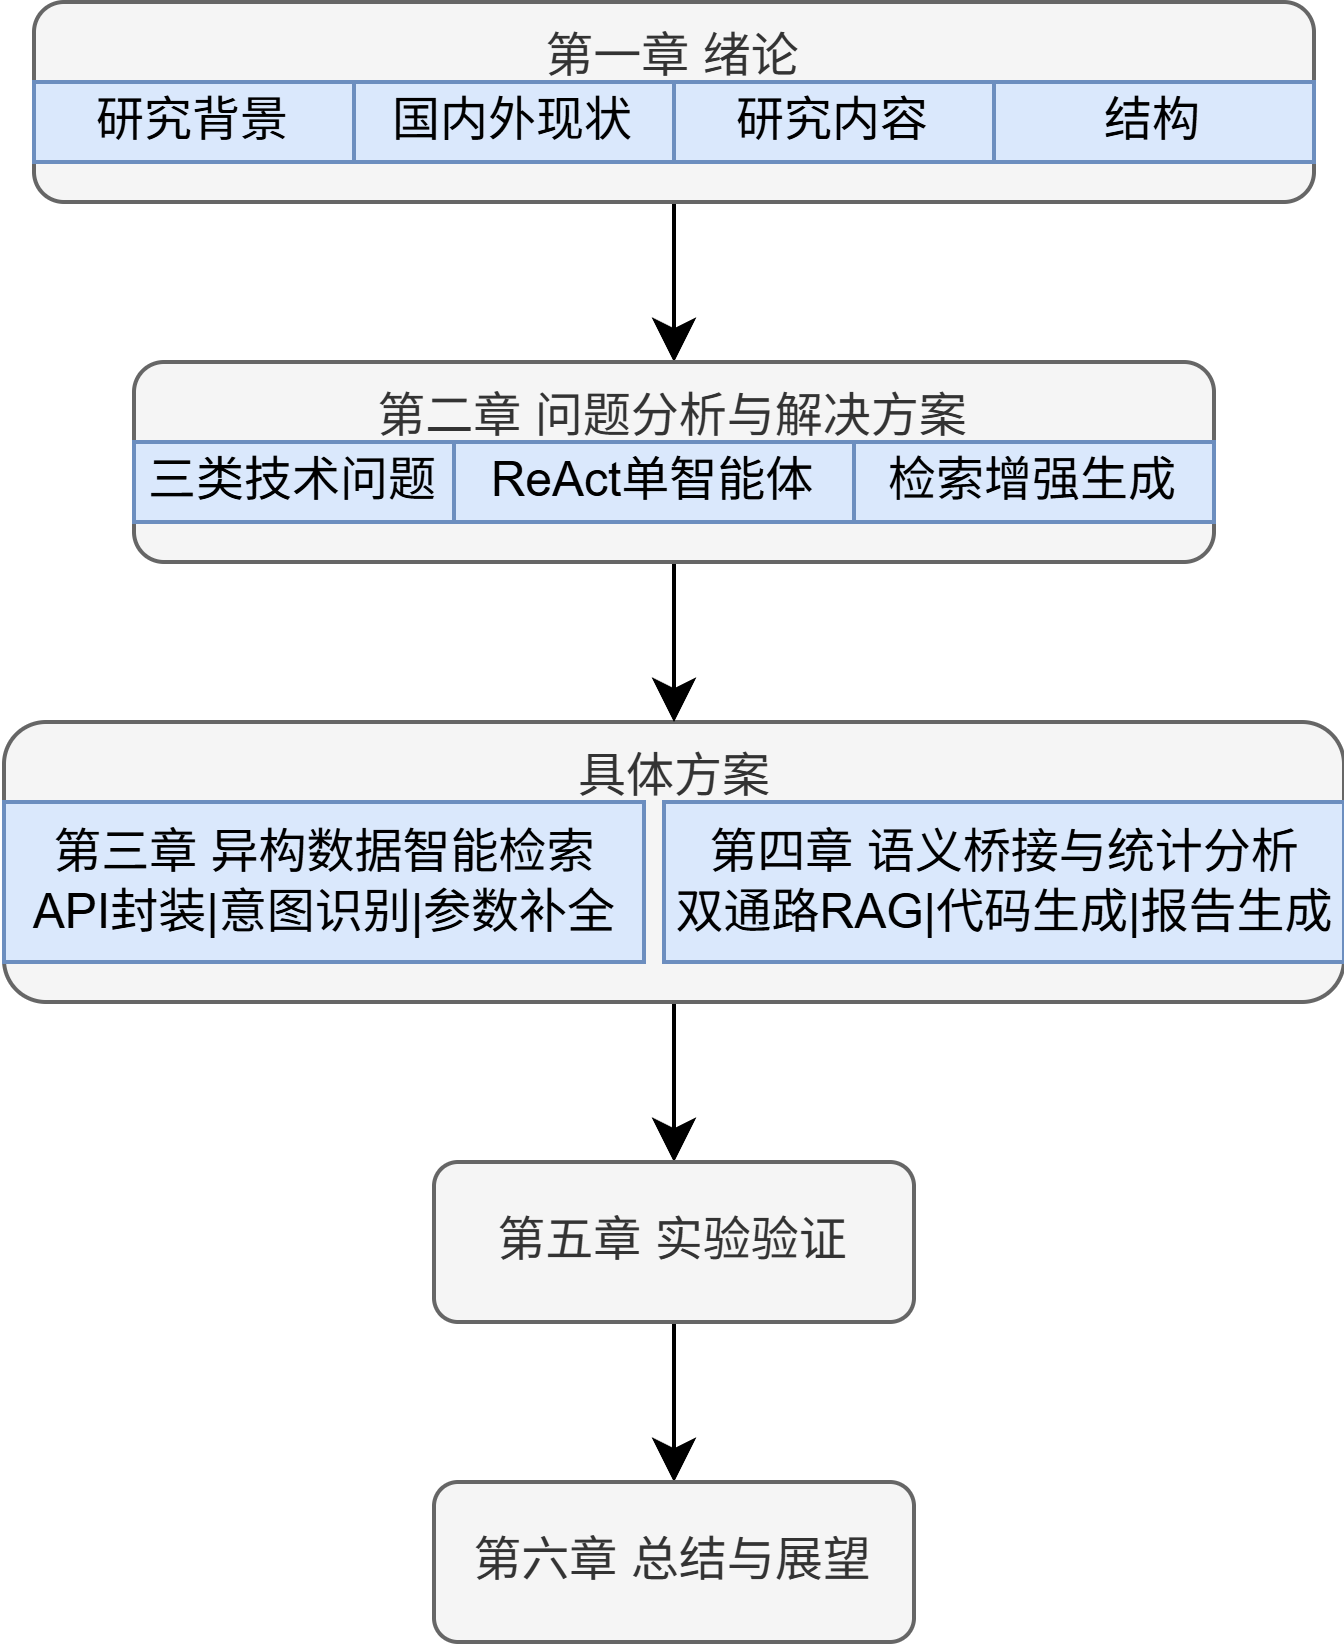
\includegraphics[width=0.5\linewidth]{figures/论文结构图}
    \caption{论文结构图}
    \label{fig:thesis-structure}
\end{figure}

第 1 章为绪论，给出研究背景与意义、综述国内外研究现状、阐述本文的
研究内容、研究方法与论文特色。第 2 章为气象预报任务技术问题分析与解决
方案，把课题按数据流向建模为指令解析、异构数据、数值与逻辑幻觉三个
研究问题，并给出基于 ReAct 范式的单智能体思维链模型作为统一的方法论
框架，以及基于 RAG 的领域知识注入与基于 Prompt 工程的工具调用约束作
为领域适配层。第 3 章为基于工具学习的异构气象数据智能检索技术，针对
指令解析问题展开，从工具学习、意图识别、参数补全三个维度构建从自然
语言查询到结构化检索请求的完整链路。第 4 章为融合语义桥接机制的气象
数据统计分析方法，针对异构数据与数值幻觉两个研究问题，给出双通路
RAG 架构、代码生成加受限沙箱执行机制以及自适应气象决策报告生成三类
核心方法。第 5 章为实验验证，按意图识别、混合检索、语义桥接、代码
执行 4 个模块层评测加 1 个 30 条端到端集成层评测的顺序展开 5 类系统
化实证。第 6 章为总结与展望，从全文总结与未来展望两个角度收束全文。

各章之间的逻辑关系可归纳为问题驱动加方法落地加实证收束的三段结构。
第 2 章是问题与方法的定义层，第 3 章至第 4 章是方法的实现层，第 5 章
是实证的验证层。指令解析问题在第 3 章落地，异构数据与数值幻觉两个
问题在第 4 章落地，所有方法的有效性由第 5 章的 5 类系统化评测共同
验证，并在第 6 章统一收束为研究结论与未来工作。

\subsubsection*{1.3.2 \quad 研究方法与技术路线}

本文采用以工程实现为主线、沿用 ReAct 范式 \cite{ref18} 的设计原则、
辅以系统化实证的研究方法。从技术路线视角看，本文构建的气象 Agent
系统按数据流向可分为接入层、处理层、知识库层与输出层四个组成部分，
整体技术栈如 \reffig{fig:tech-roadmap} 所示。

\begin{figure}[!ht]
    \centering
    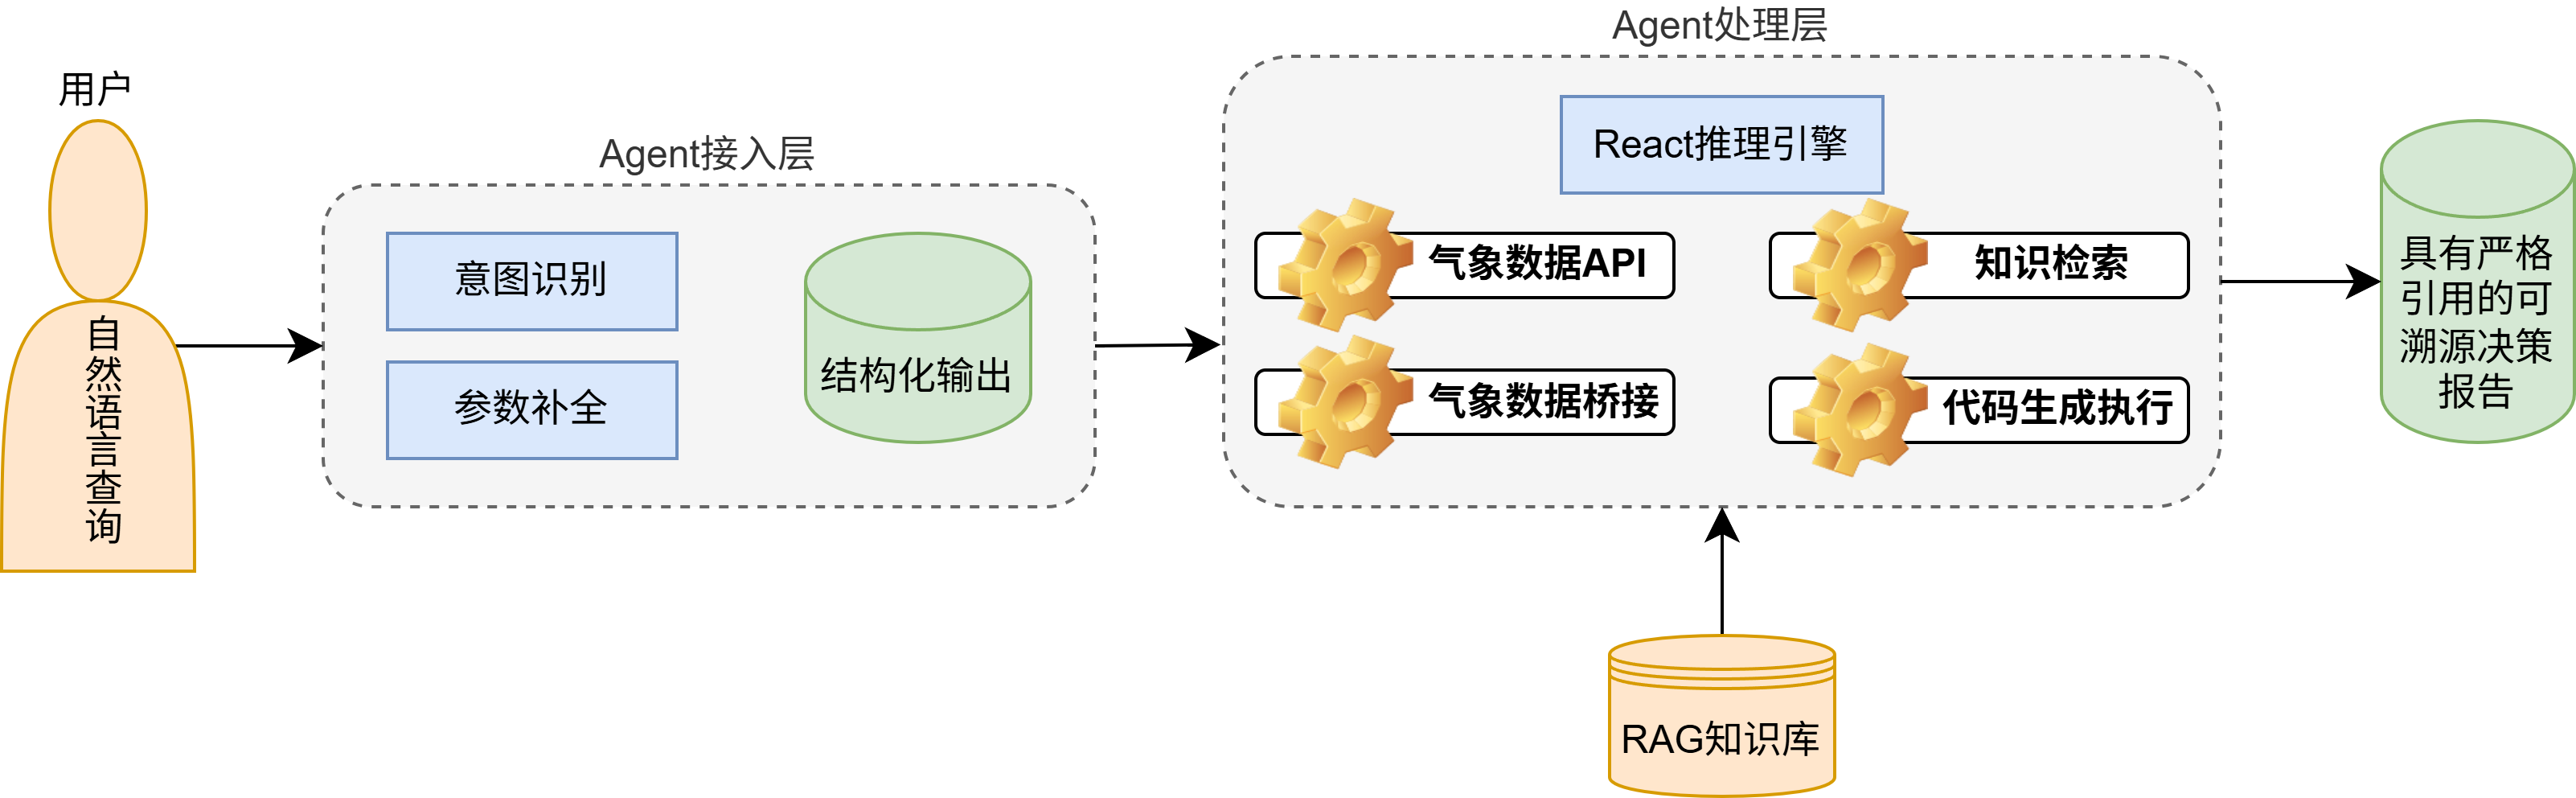
\includegraphics[width=0.95\linewidth]{figures/研究技术路线图}
    \caption{研究技术路线图}
    \label{fig:tech-roadmap}
\end{figure}

接入层负责把用户自然语言查询解析为结构化 \texttt{WeatherIntent} 对象，
由 \texttt{recognizer} 与 \texttt{completer} 两个独立模块构成意图识别
加参数补全的双阶段管线。处理层以 LangGraph 与 LangChain 0.3 的
\texttt{create\_\bk{}agent} 为推理引擎实现，集成 9 个气象 API 工具与
2 个 RAG 工具共 11 个工具单元，依据 ReAct 范式 \cite{ref18} 在每一轮
交替执行思考与行动。知识库层由向量化知识库加确定性分级器组成，对外
提供混合检索与硬链接式语义桥接两条调用通路。输出层在 ReAct 循环结束
后由大语言模型按统一提示模板组织面向决策的自然语言报告。底层大语言
模型以 SiliconFlow 平台提供的 GLM-5.1 为被测模型，温度全部置 0 以
最大化结果可重复性。

从研究路线视角看，本文的研究工作按文献调研与方案设计、模块实现、
模块层评测、集成层评测与论文撰写四个阶段递进推进。

第一阶段为文献调研与方案设计。通过研读 ReAct \cite{ref18}、思维链
\cite{ref13}、检索增强生成 \cite{ref12}、工具学习 \cite{ref21, ref28}
等核心工作形成总体方案。第二阶段为模块实现，按指令解析问题对应的
接入侧、异构数据问题对应的中段流水线、数值与逻辑幻觉问题对应的解读
侧的顺序依次落地。第三阶段为模块层评测，分别针对意图识别、检索、桥接、
代码执行 4 个模块独立设计评测集与消融对照。第四阶段为集成层评测与
论文撰写，通过 30 条真实场景用例的 \texttt{full} 档与 \texttt{ablated}
档对照验证整套系统的端到端价值，并据此完成论文核心论证闭环。

\subsubsection*{1.3.3 \quad 论文特色}

围绕上述三个研究问题与四阶段技术路线，本文给出五项特色工作，与对应
章节位置以及评测出口共同列于 \reftab{tab:contributions}。

\begin{table}[!ht]
    \centering
    \caption{本文五项特色工作与对应章节及评测概览}
    \label{tab:contributions}
    \song\fontsize{9pt}{12pt}\selectfont
    \renewcommand{\arraystretch}{0.95}
    \begin{tabular}{lll}
        \toprule
        特色 & 章节 & 关键实证 \\
        \midrule
        ReAct 单智能体气象 Agent 架构 & \ref{sec:react-paradigm} & 11 个工具集成、单进程多轮对话 \\
        工具学习驱动的异构数据检索 & \ref{chap:retrieval} & 端到端 91.4\% / 角色 100\% \\
        双通路 RAG 与语义桥接 & \ref{sec:semantic-bridge} & Top-1 85.0\% / \texttt{grade\_\bk{}id} 100\% \\
        代码生成与受限沙箱执行 & \ref{sec:code-execution} & 数值准确率 +22.2 pp \\
        多层评测体系（5 套 214 用例） & \ref{chap:evaluation} & 端到端通过率 +13.4 pp \\
        \bottomrule
    \end{tabular}
\end{table}

第一项特色是基于 ReAct 范式的气象 Agent 单智能体架构。本文采用
单智能体加显式工具学习而非多智能体协作的工程取舍，把场景编排、
出处强制、出行场景多地点对齐等约束下沉到 System Prompt，避免
了多智能体之间的状态同步与额外延迟。该架构集成 9 个气象 API 工具
加 2 个 RAG 工具共 11 个工具单元，并通过 LangGraph 的
\texttt{InMemorySaver} 与 \texttt{thread\_\bk{}id} 机制实现多轮对话
状态保持。

第二项特色是工具学习驱动的异构数据检索机制。本文为和风天气与
Open-Meteo 两类异构 API 设计统一的 Function Calling Schema,
并通过意图识别与参数补全双阶段管线把自然语言查询映射为结构化
\texttt{WeatherIntent} 对象。在 35 条评测集上端到端通过率达到
91.4\%，多地点角色识别准确率达到 100\%，证明了分层架构在容错
能力上的天然优势。

第三项特色是双通路 RAG 架构。通路 A 把向量检索与 BM25 词法检索
以可调权重融合，承担概念性查询的高召回任务；通路 B 由 5 类确定性
分级器加 \texttt{grade\_\bk{}id} 硬链接构成，承担数值到等级再到标准
引用的精确归属任务。在 60 条检索评测集与 71 条桥接评测集上,
通路 A 的 Top-1 命中率达到 85.0\%、MRR 达到 0.908，通路 B 的
\texttt{grade\_\bk{}id} 准确率与权威引用真实性同时达到 100\%，与
大语言模型自由发挥的基线在严格命中率上形成 74.6 个百分点差距。

第四项特色是基于代码生成与受限沙箱的确定性统计分析机制。本文
设计的轻量沙箱方案由大语言模型生成 \texttt{compute(data)} 顶层
函数，在白名单 builtins 加白名单模块加墙钟超时加结构化错误捕获
四重约束下执行。在 18 条覆盖 6 类统计模式的评测集上，代码执行档
数值准确率达到 88.9\%，比大语言模型自由直算高出 22.2 个百分点,
失败模式分析进一步揭示了大语言模型在伴随状态维护与离散计数任务
上的内在边界。

第五项特色是覆盖模块层与集成层的多层评测体系。本文构建了 5 份
独立评测集共 214 条用例，包含 4 个模块层评测加 1 个 30 条端到端
集成层评测。集成层评测以最终用户体验视角验证整套系统的端到端
价值，\texttt{full} 档端到端通过率为 86.7\%，相对 \texttt{ablated}
去 RAG 对照档提升 13.4 个百分点；权威标准引用率从 0\% 提升到 26.7\%；
\texttt{decision\_support} 类用例通过率从 50\% 提升到 100\%。同时
该评测也揭示了从模块层到集成层的指标衰减，构成 \ref{sec:future-work}
节未来工作的基础。
% ===== END: 草稿/1_3_主要研究内容 =====



\sectionbreak
% ============================================================ %
% 第 2 章：气象预报任务技术问题分析与解决方案
%   - 2.1 三类技术难点建模（指令解析 / 异构数据 / 数值与逻辑幻觉）
%   - 2.2 ReAct 单智能体思维链模型（含气象 Agent 总体架构图占位）
%   - 2.3 RAG 领域知识注入 + Prompt 工程优化策略
%   - 2.4 本章小结
%   - TODO: figures/agent_architecture.png 待 drawio 出图后接入 2.2 节占位框
% ============================================================ %
\seccontent
\section{气象预报任务技术问题分析与解决方案}
\label{chap:problem-modeling}

% ===== BEGIN: 草稿/2_1_技术难点建模 =====
% =============================================================================
% 2.1 气象数据检索与分析的技术难点建模
% 草稿版本：v0.1 (2026-05-05)
% 字数：约 2200 字
% 风格规则：v0.2 风格（无 \textbf / \textit / 引例括号 / 双引号 / 破折号）
% 引用：\cite{ref2, ref5, ref10, ref20, ref25}
% 图表：
%   - 表 \reftab{tab:three-questions}     三个研究问题的对照建模
%   - 表 \reftab{tab:hallucination-types} 大语言模型在气象任务中的 5 类幻觉
% 依赖宏包：booktabs / tabularx（主稿已加载）
% =============================================================================

\subsection{气象数据检索与分析的技术难点建模}
\label{sec:problem-modeling}

把大语言模型应用到气象预报数据的检索与分析这一具体业务场景，本质上是
把通用的语言模型能力嫁接到一个对数值精度、来源权威性与时空一致性都有
严格要求的垂直领域。本节按用户感知到 Agent 内部的处理顺序，把这一嫁接
过程中暴露出的技术难点抽象为三个相互独立又相互衔接的研究问题，依次为
气象任务指令解析问题、气象数据异构特征问题、大语言模型数值与逻辑幻觉
问题，并在 \reftab{tab:three-questions} 中给出三者的对照建模。本章
后续内容将给出本文的统一应对方案，第 3 章至第 4 章则是这一方案在三类
问题上的具体落地。

\begin{table}[!ht]
    \centering
    \caption{气象 Agent 三类技术问题的对照建模}
    \label{tab:three-questions}
    \song\fontsize{9pt}{12pt}\selectfont
    \renewcommand{\arraystretch}{0.95}
    \begin{tabular}{lll}
        \toprule
        研究问题 & 主要表现 & 对应章节 \\
        \midrule
        指令解析问题 & 自然语言到结构化检索参数的映射缺口 & \ref{chap:retrieval} \\
        异构数据问题 & 多源、多粒度、多要素接入与归一化 & \ref{sec:api-tooling} 与 \ref{sec:semantic-bridge} \\
        数值与逻辑幻觉问题 & 数值理解、引用编造、统计口径漂移 & \ref{sec:semantic-bridge} 与 \ref{sec:code-execution} \\
        \bottomrule
    \end{tabular}
\end{table}

\subsubsection*{2.1.1 \quad 气象任务指令解析问题}

气象 Agent 接收的输入是用户自然语言查询，输出最终需要进入工具调用层
转化为带有结构化参数的 API 请求。两端之间存在显著的形式与语义鸿沟。

第一类形式鸿沟是参数的结构化要求。和风天气 \texttt{get\_\bk{}forcast\_\bk{}weather}
要求传入 \texttt{LocationID} 加 \texttt{hours} 取值集合中的一个枚举值
\texttt{24h}、\texttt{72h} 或 \texttt{168h}；Open-Meteo 历史数据接口
要求经度纬度加起止日期的 ISO 8601 字符串。用户却倾向于使用自由
表达式例如武汉这周天气如何或者去年这个月每小时降水多少。把武汉这周
解析为 \texttt{LocationID=\bk{}101200101} 加 \texttt{hours=\bk{}168h},把去年
这个月解析为 \texttt{[2024-04-01, 2024-04-30]}，需要 Agent 同时处理
命名实体识别、相对时间消歧、参数枚举映射三类子任务。代刊等 \cite{ref5}
在大语言模型于天气预报中的应用探讨一文中也注意到，自然语言查询到
业务接口可调用形式的转换是大语言模型走向气象业务落地必须解决的
工程基础问题之一。

第二类语义鸿沟是用户表达的不完整性与角色多样性。用户提问明天天气怎么样
通常默认查询所在地，提问北京天气怎么样通常默认查询当天，提问明天早八
到晚六从武汉到成都有什么穿衣建议则隐含起点终点两个角色与对应时间段的
对齐关系。这类信息在前置 NLU 阶段如果不显式抽取，下游 ReAct 循环
会陷入猜参数的低效尝试或者直接传入错误参数。本文据此把指令解析问题拆解为意图识别加参数
补全两个相对独立的子任务，分别在 \ref{sec:intent-recognition} 节
与 \ref{sec:param-completion} 节展开。

第三类是对抗鲁棒性。用户输入并不总是合法气象查询，例如推荐部好看的
电影这类与气象无关的输入也会进入系统，需要 Agent 能识别并友好引导
而不是强行解析为某个气象意图。

\subsubsection*{2.1.2 \quad 气象数据的异构特征分析}

气象数据天然异构，且这一异构性贯穿数据接入、数据组织、数据解读三个
不同层面 \cite{ref25}。

第一是数据源异构。本文同时接入和风天气 API 与 Open-Meteo 两类数据源。
和风天气提供商业级实时观测、逐小时与逐日预报、天气预警、生活指数等
增值服务，但仅覆盖近 30 天与未来 30 天的窗口；Open-Meteo 由 European
Centre for Medium-Range Weather Forecasts 等机构维护，提供免费的
全球长期历史数据归档，时间深度可追溯到 1940 年代，但缺少天气预警与
生活指数等业务化能力。两类数据源在地理标识、参数命名、字段命名、
错误码体系上完全不一致，需要在工具层做统一封装。

第二是数据粒度异构。同一气象要素在不同接口下的时间粒度可能从分钟级
到月级跨度数个数量级，例如逐小时预报的 \texttt{precip} 字段以毫米
每小时为单位，逐日预报的 \texttt{precip} 字段以毫米每日为单位，历史
归档的 \texttt{precipitation\_\bk{}sum} 字段则是日累积量。直接把不同粒度
的数值传给大语言模型容易引发口径混乱例如把日累积 \SI{50}{mm} 当成
小时累积 \SI{50}{mm} 来判定。

第三是数据要素异构。气象要素中既有连续型如温度、湿度、降水、风速,
又有离散型如风力等级、能见度等级、生活指数等级，还有事件型如预警
信号、灾害等级。本文在 \ref{sec:semantic-bridge} 节通过双通路 RAG
架构把这一异构性吸收在确定性分类器内部，对外统一输出 \texttt{原始值
→ 分级名 → 影响描述 → 标准引用} 四元组。

气象业务对 AI 智能体范式的关注亦可见于近期国内同行的探讨，
李特等 \cite{ref2} 在中国气象学会年会上即就 AI 智能体在天气预报
业务中的应用进行了思考与探索。本文在工程实现层面把异构性的处理
内置于 Agent 内部，由工具学习模块负责跨源 API 的统一封装与
归一化、由语义桥接模块负责数值与等级口径的对齐，避免在 Agent
之外维护额外的数据中间层。

\subsubsection*{2.1.3 \quad 大语言模型的数值与逻辑幻觉}

大语言模型的训练目标本质上是以下一个 token 的预测来逼近文本概率
分布，这一目标天然导致模型在严格要求数值精度与权威引用的任务上
存在内在边界 \cite{ref10}。Hong 等 \cite{ref20} 在 Data Interpreter
中针对数据科学场景设计了以代码生成与执行为核心的 LLM Agent，其
工作从侧面表明在涉及多步统计与数值处理的任务上单纯依赖 prompt
内推理难以达到生产可用的可靠性。本文在气象领域的初步实证
（\ref{sec:bridge-eval} 节与 \ref{sec:code-eval} 节）进一步把这一
现象细化为五类典型幻觉，归纳于 \reftab{tab:hallucination-types}。

\begin{table}[!ht]
    \centering
    \caption{大语言模型在气象任务中的 5 类典型幻觉}
    \label{tab:hallucination-types}
    \song\fontsize{9pt}{12pt}\selectfont
    \renewcommand{\arraystretch}{0.95}
    \begin{tabular}{lll}
        \toprule
        幻觉类型 & 主要表现 & 实证出处 \\
        \midrule
        引用编造 & 编造 GB/T 标准号或条款号 & \ref{sec:bridge-eval} 节 \\
        分级编造 & 自创不存在的等级编号或等级名 & \ref{sec:bridge-eval} 节 \\
        数值漂移 & 数数错、舍入不一致、字段命名漂移 & \ref{sec:code-eval} 节 \\
        范围错位 & 把日累积当小时值或反之 & \ref{sec:bridge-eval} 节 \\
        场景误判 & 不应输出建议时仍输出建议 & \ref{sec:bridge-eval} 节 \\
        \bottomrule
    \end{tabular}
\end{table}

引用编造是数值与逻辑幻觉问题中最典型也最危险的一类幻觉。在
\ref{sec:bridge-eval}
节的对照实验中，大语言模型自由发挥档对 71 条评测集输出的引用条款中
仅 5.6\% 的 \texttt{grade\_\bk{}id} 完全正确，且即使引用文本看起来合理,
\texttt{must\_\bk{}cite} 关键词的严格命中率也只有 25.4\%。换言之，模型
有约四分之三的概率会以看似权威的方式给出实际错误的引用，这种真实
却错的失败模式比纯粹捏造更难被用户识别。

分级编造与引用编造紧密相关，是结构化输出场景下的另一类常见失败。
模型在被问到 \SI{35}{mm} 的降水
属于什么级别时会自创类似 \texttt{grading\_\bk{}precip\_\bk{}24h\_\bk{}strong} 这种
看起来合理但知识库中并不存在的 \texttt{grade\_\bk{}id}。这种自创编号在
形式上完全符合命名规则，足以骗过基于字符串匹配的下游引用检查。

数值漂移在 \ref{sec:code-eval} 节的代码执行评测中得到量化。在 18 条
覆盖求平均、求极值、求和、求差、计数、排序六类统计模式的评测集上,
让大语言模型直接做心算或自由生成结果，整体数值准确率为 66.7\%；
其中极值类任务准确率为 0\%，计数类任务准确率约 50\%。模型在需要维护
伴随状态的离散计数任务上失败率最高，这一观察与 Hong 等 \cite{ref20}
在 Data Interpreter 中将多步数据科学任务交由代码执行兜底的总体
设计动机一致。

范围错位与场景误判是两类相对隐蔽但同样常见的幻觉。前者源于大语言
模型缺乏稳定的单位与时间粒度记忆，在不同上下文中对相同数值的解读
会发生切换；后者源于模型倾向于在结构化输出场景下也给出建议，例如
在户外作业场景下仍输出洗车提示，违反场景过滤约束。

针对数值与逻辑幻觉问题的五类幻觉，本文不寻求通过更大模型或更复杂
prompt 来缓解,
而是通过把数值理解、引用归属、统计计算三类高风险任务从大语言模型
内部转移到外部确定性组件。\ref{sec:semantic-bridge} 节用确定性分级
加 \texttt{grade\_\bk{}id} 硬链接消除引用与分级编造，
\ref{sec:code-execution} 节用代码生成加受限沙箱执行消除数值漂移。
本文据此把这一思路概括为大语言模型只做语言组织、数值与引用让外部
组件兜底，并以模块层与端到端两个维度的实证验证其有效性。

\subsubsection*{2.1.4 \quad 三个问题的层级关系}

三个研究问题在数据流向上构成自然的层级。指令解析问题解决用户输入
到结构化请求的转化，是 Agent 流水线的入口；异构数据问题解决结构化
请求到原始数据的取数与归一化，是数据通路的中段；数值与逻辑幻觉
问题解决原始数据到自然语言决策报告的解读与表达，是 Agent 流水线
的出口。三个问题的解决方案在工程上也存在依赖关系，异构数据接入
依赖指令解析输出的结构化意图作为参数来源，语义桥接依赖工具调用
结果作为输入数值。这种依赖关系决定了本文在第 3 章先解决前两个问题
对应的接入侧任务，第 4 章再解决数值与逻辑幻觉问题对应的解读侧任务。

作为本章后续内容的承接，下一节将讨论统一这三个子问题的方法论
框架，即基于 ReAct 范式的单智能体思维链模型。

% ===== END: 草稿/2_1_技术难点建模 =====


% ===== BEGIN: 草稿/2_2_ReAct范式 =====
% =============================================================================
% 2.2 基于 ReAct 范式的单智能体思维链模型解决方案
% 草稿版本：v0.3 (2026-05-07)
%   v0.1：完成正文初稿。\reffig{fig:agent-architecture} 以 \fbox 占位框给出。
%   v0.2：接入 figures/agent_architecture.png 真实出图，移除 \fbox 占位。
%   v0.3：按导师意见 10 在 2.2.1 末段嵌入 fig:react-loop ReAct 循环图，
%        承接思考-行动-观察循环的论述并衔接 2.2.3 总体架构。
% 字数：约 2000 字
% 风格规则：v0.2 风格（无 \textbf / \textit / 引例括号 / 双引号 / 破折号）
% 引用：\cite{ref13, ref15, ref18, ref19, ref30}
% 图表：
%   - 图 \reffig{fig:react-loop}             ReAct 推理-行动-观察循环图
%   - 图 \reffig{fig:agent-architecture}     气象 Agent 总体架构图
%   - 表 \reftab{tab:single-vs-multi-agent}  单智能体与多智能体的取舍对照
% 依赖宏包：booktabs / tabularx / graphicx（主稿已加载）
% =============================================================================

\subsection{基于 ReAct 范式的单智能体思维链模型解决方案}
\label{sec:react-paradigm}

\ref{sec:problem-modeling} 节提出的三个研究问题不能由任意单一方法
独立解决。意图解析需要语言理解能力，工具调度需要结构化输出能力,
数值与引用兜底需要外部组件协作能力。本节论证 ReAct 范式作为统一
方法论框架的合理性，并给出本文气象 Agent 在单智能体形态下的总体
架构。

\subsubsection*{2.2.1 \quad 思维链与 ReAct 推理 - 行动 - 观察循环}

思维链 \cite{ref13} 是把复杂任务分解为一系列中间推理步骤的提示
工程范式。其核心观察是大语言模型在隐式直接生成最终答案时常常出错,
但如果通过提示让模型显式写出中间推理步骤，则能在算术、常识推理
与符号操作任务上取得显著的准确率提升。Wei 等 \cite{ref13} 提出的
思维链提示方法奠定了大语言模型作为推理引擎的基本能力假设。但纯
思维链的局限是模型只能依赖训练时的内部知识，无法访问实时信息或
执行外部计算，因此对于气象任务这种强依赖最新数据与权威标准的场景
不能直接套用。

ReAct \cite{ref18} 把思维链与工具调用结合起来。模型在每一轮的输出
分为思考 (Thought) 与行动 (Action) 两部分，思考用于分析当前状态
并决定下一步行动，行动以结构化形式给出工具名与参数；外部环境执行
该行动并把结果作为观察 (Observation) 返回给模型，模型据此进行下一
轮思考。这种推理 - 行动 - 观察的交替循环把模型从纯生成者升级为
带工具的推理者，原本无法在内部完成的任务被拆解为多步外部协作。
本文气象 Agent 的核心循环采用 LangGraph 框架 \cite{ref15} 实现这一
范式，所有 11 个气象工具加 RAG 工具均通过同一个工具节点暴露给模型,
模型在每一轮自由选择是否调用、调用哪一个、传入什么参数。
ReAct 推理 - 行动 - 观察循环的整体形态见 \reffig{fig:react-loop}。

\begin{figure}[!ht]
    \centering
    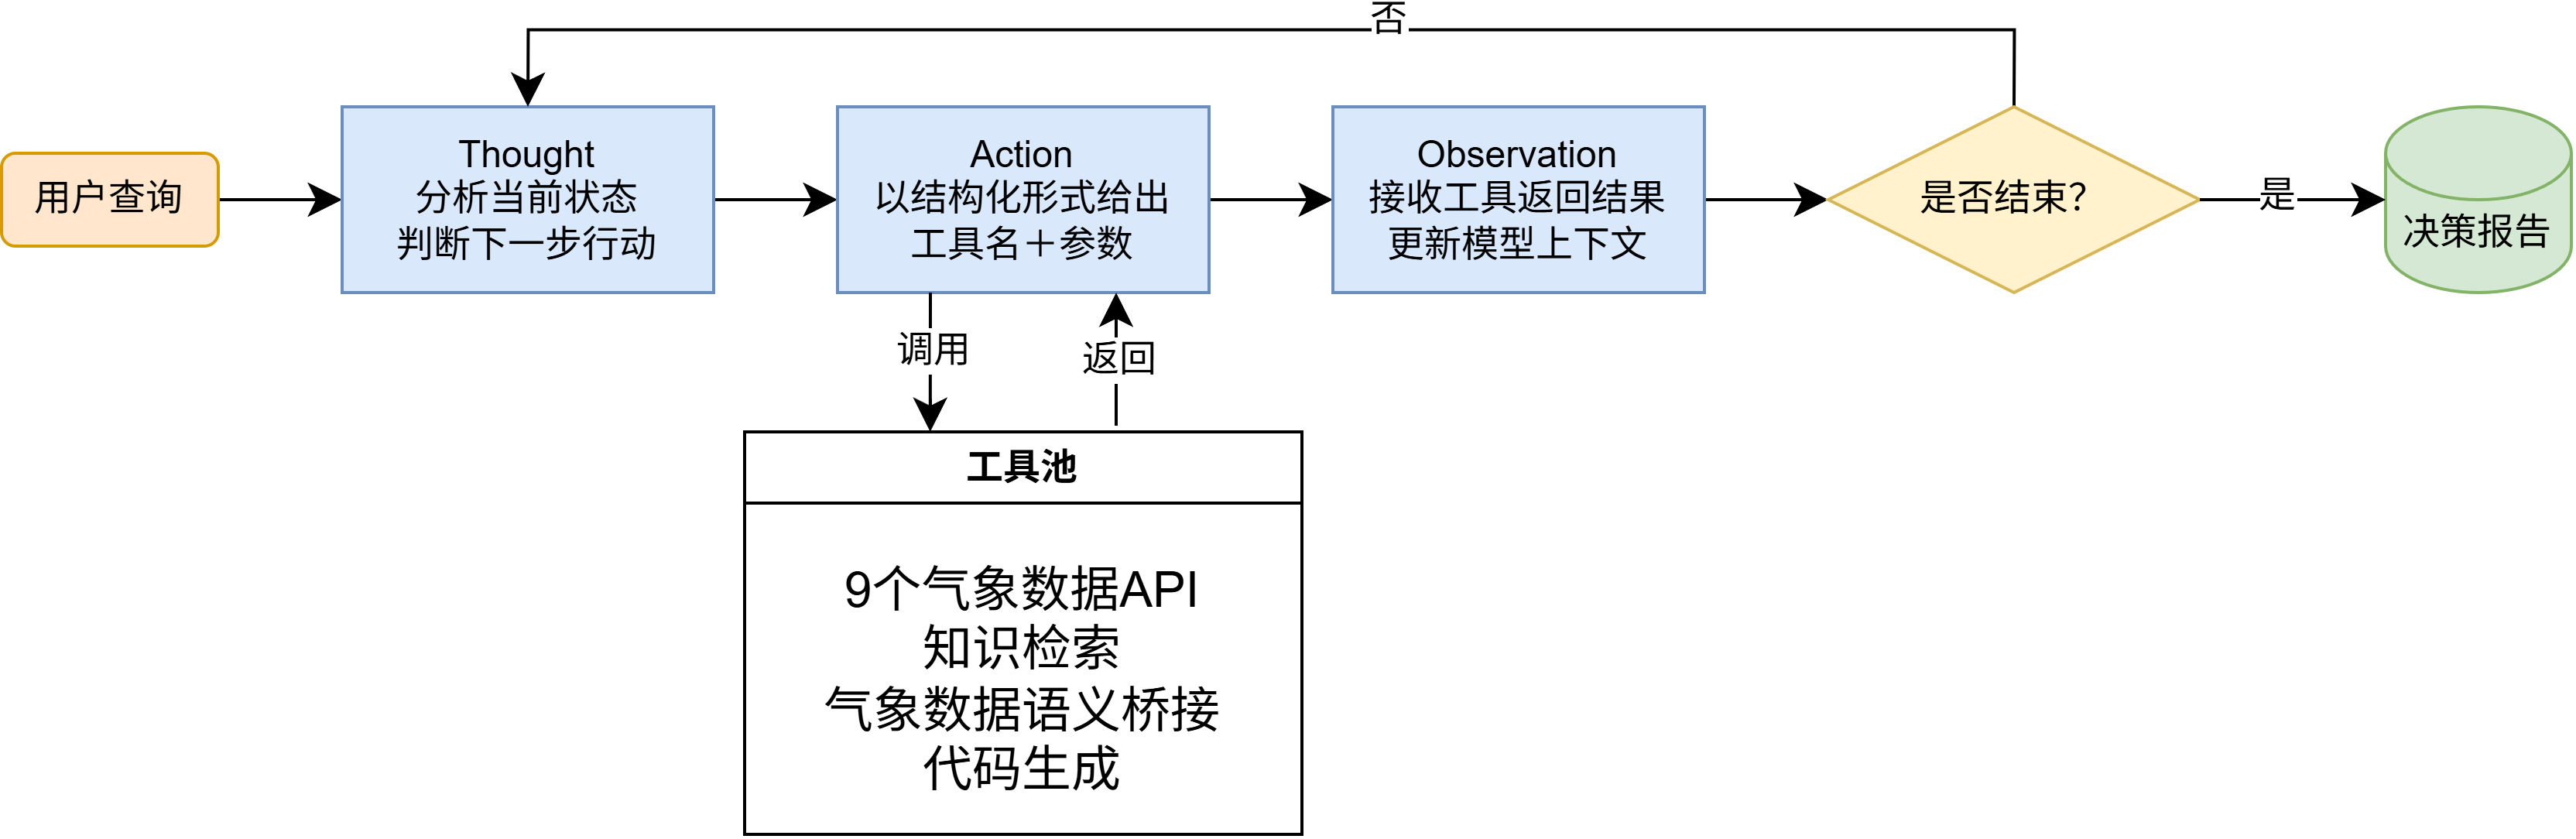
\includegraphics[width=0.85\linewidth]{figures/ReAct循环图}
    \caption{ReAct 推理-行动-观察循环示意图}
    \label{fig:react-loop}
\end{figure}

针对气象 Agent 的具体场景，本文在原始 ReAct 循环之上增加了三处
工程改造。第一是把意图识别与参数补全前置到 ReAct 循环之外作为
独立的 NLU 阶段，让 ReAct 循环以结构化 \texttt{WeatherIntent}
作为输入而非裸用户问题。这一改造对应指令解析问题，避免模型在
ReAct 循环内部承担意图与参数推理的双重负担。第二是把语义桥接
\texttt{bridge\_\bk{}weather\_\bk{}data} 工具与代码生成执行流水线作为
ReAct 循环可调用的子组件，让模型可以在拿到原始数值后主动选择是否
桥接、是否生成统计代码。这一改造对应数值与逻辑幻觉问题。第三是
显式记忆与状态保持。LangGraph 的 \texttt{InMemorySaver} 加
\texttt{thread\_\bk{}id} 机制让多轮对话中模型能继承上一轮的工具调用
结果与意图状态，避免每轮重复 search\_city 等基础查询。

Tree of Thoughts \cite{ref30} 在 ReAct 之外提出了搜索树形态的多
分支推理范式，更适合数学证明与谜题求解类任务。气象 Agent 的工具
调用任务在搜索深度与分支度上都不算大，单链 ReAct 循环已能覆盖
绝大多数场景，本文据此选择 ReAct 而非 Tree of Thoughts 作为基础
推理范式。

\subsubsection*{2.2.2 \quad 单智能体与多智能体的工程取舍}

近年来的 Agent 系统出现了从单智能体向多智能体协作演进的趋势。
AutoGen \cite{ref19} 提出可定制对话格局的多智能体框架，让多个具有
不同角色的 Agent 通过结构化对话协作完成复杂任务。本文不采用多
智能体方案，主要基于以下三点工程取舍，详见
\reftab{tab:single-vs-multi-agent}。

\begin{table}[!ht]
    \centering
    \caption{气象 Agent 单智能体与多智能体的工程取舍对照}
    \label{tab:single-vs-multi-agent}
    \song\fontsize{9pt}{12pt}\selectfont
    \renewcommand{\arraystretch}{0.95}
    \begin{tabular}{lll}
        \toprule
        维度 & 单智能体 & 多智能体 \\
        \midrule
        响应延迟 & 单进程内部循环 & 多 agent 间消息往返 \\
        状态同步 & 单一 \texttt{thread\_\bk{}id} 自动维护 & 需要显式协议 \\
        调试粒度 & 单条工具调用栈 & 跨 agent 日志关联 \\
        架构复杂度 & ReAct 单循环 & 角色定义加调度策略 \\
        适合任务 & 工具调用为主的查询 & 子任务分工明显的科研工作流 \\
        \bottomrule
    \end{tabular}
\end{table}

第一是响应延迟。气象 Agent 的典型查询从用户提问到最终回答需要在 5 至
15 秒内完成多步工具调用，目标用户对实时性的容忍度较低。多智能体
之间的消息传递引入额外的进程间或网络往返，对响应延迟敏感的查询
任务不友好。

第二是状态同步成本。气象 Agent 在多轮对话中需要保持地点状态、时间
状态、上次查询结果三类记忆。单智能体形态下这些状态由 LangGraph 的
\texttt{InMemorySaver} 在单一 \texttt{thread\_\bk{}id} 下自动累积，模型
不需要显式管理。多智能体形态下则必须额外定义状态同步协议，让规划
者、执行者、报告者三类角色看到一致的状态视图，工程开销显著上升。

第三是调试与可观测性。本文 5 套评测脚本统一以 ReAct 循环为入口,
单智能体形态下评测脚本可以直接复用 \texttt{run\_\bk{}agent} 函数,
故障定位时只需检查单一循环的中间状态。多智能体形态下故障可能发生
在任意子 Agent，需要跨 Agent 日志关联，调试成本与集成层不确定性
都会上升。

需要指出的是，本文的工具学习与语义桥接两个模块本身可以视为内嵌于
单智能体的子能力单元，承担了多智能体框架中规划者与执行者的部分
职责。这种把多智能体的角色专门化在单智能体内部以模块形式落地的
做法，在气象 Agent 这种工具调用为主的场景下既能保留模块化优势,
又规避了多智能体的延迟与同步开销。

\subsubsection*{2.2.3 \quad 气象 Agent 总体架构}

按上述方法论选型，本文气象 Agent 的总体架构由四个层次构成，整体
组件关系见 \reffig{fig:agent-architecture}。

\begin{figure}[!ht]
    \centering
    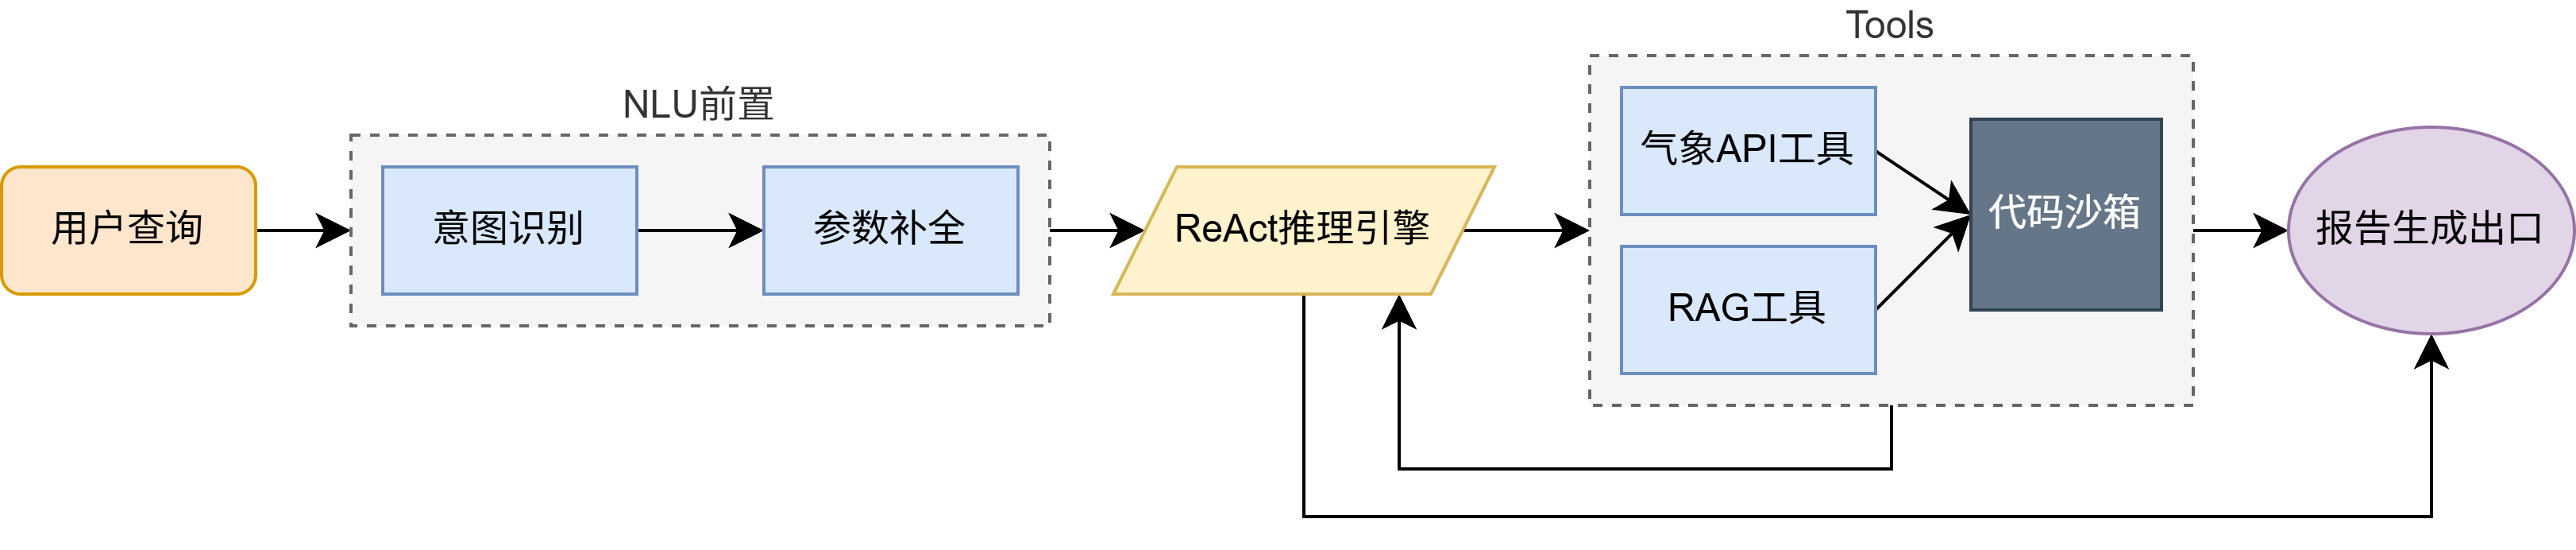
\includegraphics[width=\linewidth]{figures/agent_architecture}
    \caption{气象 Agent 总体架构示意图}
    \label{fig:agent-architecture}
\end{figure}

第一层是 NLU 前置层，由 \texttt{src/\bk{}intent/\bk{}recognizer.\bk{}py} 与
\texttt{src/\bk{}intent/\bk{}completer.\bk{}py} 两个模块构成，负责把用户自然语言
查询解析为 \texttt{WeatherIntent} 对象。这一层独立于 ReAct 循环
之外，让语言理解与工具执行解耦，便于独立评测与诊断（详见
\ref{chap:retrieval} 章）。

第二层是 ReAct 推理引擎，由 LangGraph \cite{ref15} 的
\texttt{create\_\bk{}agent} 实例化，以 SiliconFlow 提供的 GLM-5.1 为
底层大语言模型。推理引擎接收 NLU 前置层注入的结构化意图作为
首条用户消息，按 ReAct 范式 \cite{ref18} 在每一轮交替执行思考与
行动。System Prompt 以 117 行的长度承担工具调用规则、出行场景
推理规则、RAG 调用约束、输出规范四类硬约束，详见
\ref{sec:rag-prompt} 节。

第三层是工具与组件层，包含 11 个工具单元。9 个 \texttt{weather\_\bk{}api}
工具覆盖实时观测、逐小时与逐日预报、天气预警、生活指数、历史数据
六类业务场景；\texttt{search\_\bk{}knowledge} 工具从混合检索的 RAG
知识库中召回与查询相关的术语定义、分级标准、作业规范；
\texttt{bridge\_\bk{}weather\_\bk{}data} 工具把工具返回的原始数值经过确定性
分类器与 \texttt{grade\_\bk{}id} 硬链接转换为带引用源的语义标签。
此外，代码生成器与受限沙箱执行器作为第二级组件由前述工具按需
触发，承担确定性统计计算的兜底职责。

第四层是报告生成出口。Agent 在完成工具调用与中间推理后，由 LLM
按统一提示模板组织最终回答，要求显式引用知识库或桥接结果中的
权威条款，并在场景化模板下输出穿衣建议、出行建议、户外作业建议
或极端天气预警等结构化决策内容。

四个层次中，第一层与第三层的桥接、代码生成两个组件对应于本文的三
项核心特色（双阶段 NLU、双通路 RAG、代码生成与沙箱），第二层是
方法论框架，第四层是面向用户的最终出口。本文据此在第 3 章展开
第一层与第三层的工具学习子集，在第 4 章展开第三层的语义桥接、
代码生成与报告生成子集，在第 5 章对四个层次进行模块层与集成层
两个维度的系统化实证。

% ===== END: 草稿/2_2_ReAct范式 =====


% ===== BEGIN: 草稿/2_3_RAG与Prompt策略 =====
% =============================================================================
% 2.3 基于 RAG 的领域知识注入与 Prompt 工程优化策略
% 草稿版本：v0.1 (2026-05-05)
% 字数：约 2000 字
% 风格规则：v0.2 风格（无 \textbf / \textit / 引例括号 / 双引号 / 破折号）
% 引用：\cite{ref4, ref12, ref18, ref20, ref24}
% 图表：
%   - 表 \reftab{tab:kb-three-categories}    知识库三类条目说明
%   - 表 \reftab{tab:prompt-modules}         System Prompt 6 段模块化设计
% 依赖宏包：booktabs / tabularx（主稿已加载）
% =============================================================================

\subsection{基于 RAG 的领域知识注入与 Prompt 工程优化策略}
\label{sec:rag-prompt}

前节给出的 ReAct 单智能体框架本身只是方法论骨架，要在气象任务上
落地仍需解决两个具体问题：领域知识从何处获取、如何让大语言模型
在合适的时机调用合适的工具。本节分别给出两个问题
对应的工程方案：基于 RAG 的领域知识注入与基于 Prompt 工程的工具
调用约束。这两个方案在功能上正交而在使用上互补，共同构成 ReAct
循环之上的领域适配层。

\subsubsection*{2.3.1 \quad 领域知识库的三类条目设计}

气象领域的权威知识具有强结构化、强出处、强版本化三个特征。强结构化
体现为大量阈值表、分级表、生活指数等级表，例如降水量等级、蒲福
风级、空气质量指数等。强出处体现为绝大多数业务规范都来自国家标准、
行业标准或国际组织规范，例如 GB/T 28592-2012 降水量等级、Beaufort
wind force scale 等。强版本化体现为同一标准会在不同年份发布修订版,
例如 GB/T 21987-2017 寒潮等级取代了早期的 GB/T 20484。这三个特征
要求知识库本身必须做到条目化、出处化、版本化的设计 \cite{ref24}。

本文据此把领域知识库划分为三类条目，每类对应不同的 RAG 调用场景,
详见 \reftab{tab:kb-three-categories}。

\begin{table}[!ht]
    \centering
    \caption{领域知识库三类条目的设计原则与典型 RAG 调用场景}
    \label{tab:kb-three-categories}
    \song\fontsize{9pt}{12pt}\selectfont
    \renewcommand{\arraystretch}{0.95}
    \begin{tabular}{lll}
        \toprule
        类别 & 用途 & 典型查询触发 \\
        \midrule
        \texttt{term\_\bk{}definition} & 气象术语定义 & 雷暴是什么、台风等级是什么 \\
        \texttt{grading\_\bk{}standard} & 数值分级阈值 & 35 mm 算什么级别、7 级风的影响 \\
        \texttt{operation\_\bk{}guideline} & 作业 / 出行规范 & 6 级风是否停止高空作业 \\
        \bottomrule
    \end{tabular}
\end{table}

\texttt{term\_\bk{}definition} 类承担概念性查询的 RAG 召回职责。当用户
直接询问某个气象术语含义时，通路 A 的 \texttt{search\_\bk{}knowledge}
工具基于向量加 BM25 的混合检索从该类条目中召回 Top-K，作为大语言
模型生成解释文本的上下文。

\texttt{grading\_\bk{}standard} 类承担数值分级与引用归属的 RAG 召回
职责。这一类条目的 \texttt{id} 字段被设计为机器可解析的硬链接键,
例如 \texttt{grading\_\bk{}precip\_\bk{}24h\_\bk{}rainstorm} 表示 24 小时降水量的
暴雨级别。通路 B 的确定性分类器通过 \texttt{grade\_\bk{}id} 字段直接
查表，绕过向量相似度，从源头消除数值分级的归属错误。

\texttt{operation\_\bk{}guideline} 类承担作业适宜性与场景过滤的知识
注入职责。这一类条目附带 \texttt{applicable\_\bk{}scene} 字段，例如
高空作业、户外运动、洗车、播种等，让 \texttt{bridge\_\bk{}weather\_\bk{}data}
工具能根据用户输入的 \texttt{scene} 参数裁剪不相关的建议，避免
\ref{sec:problem-modeling} 节描述的场景误判幻觉。

每条 JSONL 记录强制带出处三元组（机构、文件名、条款号）加可信度
标签（\texttt{official} 国家标准、\texttt{industry} 行业标准、
\texttt{common} 业内惯例）加版本号三类元数据。这种元数据完整性
是 \ref{sec:bridge-eval} 节实证中通路 B 的 \texttt{citation} 真实性
能达到 100\% 的根本前提。黄冰 \cite{ref4} 在面向古生物学领域构建
基于 RAG 的知识问答系统时，亦展示了垂直领域中以结构化条目承载
专业知识的工程价值。

\subsubsection*{2.3.2 \quad 双通路 RAG 的设计动机简述}

通路 A 的混合检索 \cite{ref12} 与通路 B 的确定性分级在功能上互补
的具体设计动机将在 \ref{sec:semantic-bridge} 节展开。本节仅说明
为何只用通路 A 不够。

向量检索对相邻阈值条目的排序不稳定。例如查询 35 mm 降水量等级，
向量检索可能召回中雨、大雨、暴雨三个相邻档位的条目，最终归属到
哪一个取决于嵌入模型的具体训练数据，无法做到与国家标准 100\%
一致。Gao 等 \cite{ref24} 在 RAG 综述中将 RAG 系统沿 Naive、
Advanced 与 Modular 三个范式梳理，并把面向具体任务定制检索与
生成模块视为 Modular RAG 的典型形态。本文据此引入通路 B 的
确定性分级，通过 if-elif 分支匹配显式的阈值范围，保证数值到
分级的归属在工程上 100\% 可控，可视为针对气象数值阈值任务定制
的一类 Modular RAG 实例。

\subsubsection*{2.3.3 \quad System Prompt 的模块化设计}

ReAct 循环 \cite{ref18} 的输出质量高度依赖 System Prompt 的设计。
本文 \texttt{src/\bk{}config/\bk{}settings.\bk{}py} 中的 \texttt{SYSTEM\_\bk{}PROMPT}
共 117 行，按功能划分为 6 个模块，详见 \reftab{tab:prompt-modules}。
模块化设计的工作目标是让大语言模型在每一轮思考时能精确定位需要
参考的规则段落，避免长 Prompt 中的相互干扰，这一按子问题拆分约束
的工程思路与 Hong 等 \cite{ref20} 在 Data Interpreter 中按子问题
分层组织 Agent 推理与执行的总体策略在精神上一致。

\begin{table}[!ht]
    \centering
    \caption{System Prompt 的 6 段模块化设计}
    \label{tab:prompt-modules}
    \song\fontsize{9pt}{12pt}\selectfont
    \renewcommand{\arraystretch}{0.95}
    \begin{tabular}{lll}
        \toprule
        模块 & 功能 & 行数 \\
        \midrule
        可用工具清单 & 11 个工具的功能与触发条件 & 27 行 \\
        工具使用规则 & 工具组合与调用顺序约束 & 13 行 \\
        RAG 知识检索规则 & 数据与依据分离原则 & 9 行 \\
        语义桥接调用约束 & 数值到分级的强制桥接路径 & 7 行 \\
        出行场景推理规则 & 多地点角色与时段对齐 & 8 行 \\
        输出规则 & 引用与建议的最终格式约束 & 6 行 \\
        \bottomrule
    \end{tabular}
\end{table}

第一段是工具清单。每个工具的描述包含名称、功能、参数三要素，并
按数据查询、知识检索、语义桥接三类分组。\texttt{search\_\bk{}knowledge}
工具的描述明确列出 4 类应主动调用的场景，让大语言模型在思考时
能自我提示是否需要检索。

第二段是工具使用规则。这一段把 9 类典型查询与对应工具组合显式
列出，例如问现在天气调用 \texttt{get\_\bk{}current\_\bk{}weather}、问几点
天气调用 \texttt{get\_\bk{}forcast\_\bk{}weather}。这种典型场景到工具的
映射为 ReAct 循环的初始决策提供了启发式锚点。

第三段是 RAG 知识检索规则。本段强调数据与依据的分离原则：天气
工具给出现在 30 mm 降水这种事实数据，
\texttt{search\_\bk{}knowledge} 与 \texttt{bridge\_\bk{}weather\_\bk{}data}
给出 30 mm 属于大雨这种分级依据，两者结合才能给出准确解读。这
一原则在工程上转化为对模型的两条硬约束：最终回答必须显式引用
出处；遇到 X 算什么级别的判定必须先调用 RAG 而非凭空给出。

第四段是语义桥接调用约束。这一段进一步细化数值场景下的工具
路径：用户问概念定义直接调用 \texttt{search\_\bk{}knowledge}，
用户问今天明天数值且需要建议先调用天气工具再调用桥接，用户问某
数值算什么级别直接调用桥接。三类路径共同构成对数值与逻辑幻觉问题
的强制拦截机制。

第五段是出行场景推理规则。这一段处理 \texttt{travel\_\bk{}advice}
意图下的多地点角色对齐，明确出发时段查出发地、到达时段查目的地的
工程约束。这一段的源起是 README §7.1 描述的早期失败案例：用户问
明天早八到晚六从武汉到成都的穿衣建议，初版 Agent 错误地查询了成都
早八的天气而非武汉。

第六段是输出规则。本段约束最终回答必须做到精准定位时间地点参数、
预警优先提示、引用出处必须显式保留三件事。这是面向终端用户的格式
化约束，与第三、四段的过程性约束形成最终输出闭环。

\subsubsection*{2.3.4 \quad Few-shot 示例与 Prompt 的协同}

在 System Prompt 之外，本文在 \texttt{INTENT\_\bk{}RECOGNIZER\_\bk{}PROMPT}
与 \texttt{COMPLETER\_\bk{}PROMPT} 中分别使用了 few-shot 示例引导
意图识别与参数补全的输出格式（详见 \ref{chap:retrieval} 章）。
few-shot 的选择遵循三条原则：第一是覆盖全部 9 类意图，每类至少
一个示例；第二是覆盖三类典型异常，包括地点缺失、时间缺失、对抗
查询；第三是示例答案与 Pydantic schema 严格一致，让模型从示例中
学到合法字段集与合法枚举值。

few-shot 与 System Prompt 的关系是抽象规则与具体范例的互补。
System Prompt 给出原则性约束让模型知道应该做什么，few-shot 给出
范例让模型知道应该怎么做。在 \ref{sec:intent-eval} 节的实证中,
两种 Prompt 形态共同支撑了 35 条评测集上 91.4\% 的端到端通过率
与 100\% 的地点角色识别率。

\subsubsection*{2.3.5 \quad 与三个研究问题的关联}

本节给出的 RAG 与 Prompt 策略与三个研究问题之间的关联可以归纳
如下。指令解析问题依赖 \texttt{INTENT\_\bk{}RECOGNIZER\_\bk{}PROMPT} 与
\texttt{COMPLETER\_\bk{}PROMPT} 中的工具映射段落，模型据此输出可
执行的结构化意图。异构数据问题依赖 System Prompt 第二段的工具
组合规则与第五段的出行场景对齐规则，模型据此能在多源、多时段、
多角色的查询下选择正确的工具组合。数值与逻辑幻觉问题则同时依赖
RAG 知识库的元数据严谨性与 System Prompt 第三、四段的强制桥接
路径，前者保证引用可追溯，后者保证桥接被实际触发。三类策略
互相加强，构成本文方法论框架在工程层面的最终落地。

% ===== END: 草稿/2_3_RAG与Prompt策略 =====


% ===== BEGIN: 草稿/2_4_本章小结 =====
% =============================================================================
% 2.4 本章小结
% 草稿版本：v0.1 (2026-05-05)
% 字数：约 500 字
% 风格规则：v0.2 风格（无 \textbf / \textit / 引例括号 / 双引号 / 破折号）
% 引用：暂无新增引用
% 依赖宏包：booktabs / tabularx（主稿已加载）
% =============================================================================

\subsection{本章小结}
\label{sec:problem-summary}

本章在第 1 章绪论给出的研究背景与文献综述基础上，把基于 AI 智能体的
气象预报数据检索与分析这一总体研究课题分解为三个相互独立又依次衔接
的研究问题，并给出了本文统一的方法论框架与领域适配层。

\ref{sec:problem-modeling} 节把课题中的技术难点按数据流向建模为
气象任务指令解析、气象数据异构特征、大语言模型数值与逻辑幻觉
三个具体问题。指令解析问题关注用户输入到结构化请求的转化，需要
处理参数结构化、表达不完整性、对抗鲁棒性三类子任务；异构数据
问题关注结构化请求到原始数据的取数与归一化，需要解决数据源、
数据粒度、数据要素三个层面的异构性；数值与逻辑幻觉问题关注原始
数据到自然语言决策报告的解读与表达，需要应对引用编造、分级编造、
数值漂移、范围错位、场景误判 5 类典型幻觉。三个问题在工程上构成
依赖关系，异构数据问题依赖指令解析输出的结构化意图，数值与逻辑
幻觉问题依赖工具调用返回的结果。

\ref{sec:react-paradigm} 节给出统一应对三类问题的方法论框架：
基于 ReAct 范式的单智能体思维链模型。本文在原始 ReAct 循环之上
增加了 NLU 前置、桥接子组件可调用、显式记忆三处工程改造，并通过
单智能体与多智能体的工程取舍对照论证了在响应延迟、状态同步、
调试可观测性三个维度选择单智能体的合理性。气象 Agent 的总体架构
划分为 NLU 前置层、ReAct 推理引擎层、工具与组件层、报告生成出口
四个层次，覆盖从用户输入到决策输出的完整流水线。

\ref{sec:rag-prompt} 节给出方法论框架在领域上的具体落地：基于
RAG 的领域知识注入与基于 Prompt 工程的工具调用约束。前者把
领域知识库划分为术语定义、分级标准、作业规范三类条目，强制要求
出处三元组加可信度标签加版本号的元数据完整性；后者把 117 行
\texttt{SYSTEM\_\bk{}PROMPT} 模块化为工具清单、工具使用规则、RAG 检索
规则、桥接调用约束、出行场景推理规则、输出规则 6 段，与
few-shot 示例形成抽象规则与具体范例的互补关系。

本章给出的问题建模、方法论框架与领域适配层是后续 3 至 5 章具体
方法落地的总体指南。第 3 章在 NLU 前置层与工具学习层落地指令解析
与异构数据接入两个研究问题，第 4 章在工具与组件层落地数值与逻辑
幻觉问题以及最终报告生成出口，第 5 章对四个层次进行模块层加集成
层的系统化实证。

% ===== END: 草稿/2_4_本章小结 =====



\sectionbreak
% ============================================================ %
% 第 3 章：基于工具学习的异构气象数据智能检索技术（对应指令解析与异构数据接入）
%   - 3.1 气象 API 描述与封装
%   - 3.2 意图识别与指令化
%   - 3.3 缺失参数补全
%   - 3.4 本章小结
% ============================================================ %
\seccontent
\section{基于工具学习的异构气象数据智能检索技术}
\label{chap:retrieval}

% ===== BEGIN: 草稿/3_1_API封装 =====
% =============================================================================
% 3.1 气象 API 的描述与封装
% 草稿版本：v0.2 (2026-05-07)
%   v0.1：完成正文初稿。
%   v0.2：按导师意见 8 在 3.1.1 末段嵌入 fig:api-unified-wrapper 异构 API
%        统一封装层结构图，把"上层 ReAct Agent / 中间统一封装层 / 底层
%        和风+Open-Meteo 双源" 三层结构可视化。
% 字数：约 1700 字
% 风格规则：v0.2 风格（无 \textbf / \textit / 引例括号 / 双引号 / 破折号）
% 引用：\cite{ref3, ref11, ref21, ref28}
% 图表：
%   - 图 \reffig{fig:api-unified-wrapper}   异构 API 统一封装层结构图
%   - 表 \reftab{tab:api-tools-overview}    9 个 weather_api 工具汇总
% 依赖宏包：booktabs / tabularx / graphicx（主稿已加载）
% =============================================================================

\subsection{气象 API 的描述与封装}
\label{sec:api-tooling}

工具学习是大语言模型与外部世界交互的桥梁，其核心思想是把外部 API 包装
为大语言模型可识别、可调用的工具单元 \cite{ref21}。本章针对指令
解析问题所定义的气象数据智能检索任务，沿用工具学习范式分三步建立
从自然语言查询到结构化检索结果的完整链路：从底层异构 API 的描述
与封装，到自然语言查询的结构化意图识别，再到缺失检索参数的上下文
推理与动态补全。本节先讨论其中底层异构 API 的描述与封装环节。

\subsubsection*{3.1.1 \quad 异构气象数据源的统一接入}

气象数据源天然具有异构性。本文同时接入了和风天气 API 与 Open-Meteo
两类异构数据源以覆盖不同业务场景。和风天气提供商业级实时观测、逐小时
与逐日预报、天气预警、生活指数等服务，接口稳定但仅覆盖近期与未来
30 天。Open-Meteo 由欧洲气象研究机构维护，提供免费的全球长期历史
数据归档，时间深度可追溯到 1940 年代，但缺少天气预警与生活指数等
增值服务。两类数据源的接口协议、参数命名、字段命名、错误码体系都
不一致，例如和风天气使用 \texttt{LocationID} 作为地点标识符并以
\texttt{code} 字段表示状态，而 Open-Meteo 直接以纬度经度为参数并
以 \texttt{error} 字段返回错误描述。林怡等 \cite{ref3} 在面向
RESTful API 的 AI 智能体工作中也指出，API 层的描述差异与字段
异构会显著影响智能体识别与调用外部接口的可靠性，这一观察在多源
气象 API 场景下的工程意义同样成立。

本文采用统一的工具签名层封装两类异构 API，对外暴露相同的接口风格
与返回结构。所有工具实现位于 \texttt{src/\bk{}tools/\bk{}weather\_\bk{}api.\bk{}py}，
通过 \texttt{@tool} 装饰器导出为可被 LangChain Agent 自动识别的
function 工具。工具内部统一处理 HTTP 请求、状态码校验、错误兜底
与字段重命名四类细节。例如和风天气返回的 \texttt{precip} 是带
\texttt{mm} 单位的字符串而 Open-Meteo 返回的是浮点数值，封装层
统一格式化为 \texttt{X.\bk{}X mm} 字符串以便下游统一消费。这种封装把
数据源异构性吸收在工具实现内部，对上层意图识别与 Agent 编排完全
透明，整体三层结构关系见 \reffig{fig:api-unified-wrapper}。

\begin{figure}[!ht]
    \centering
    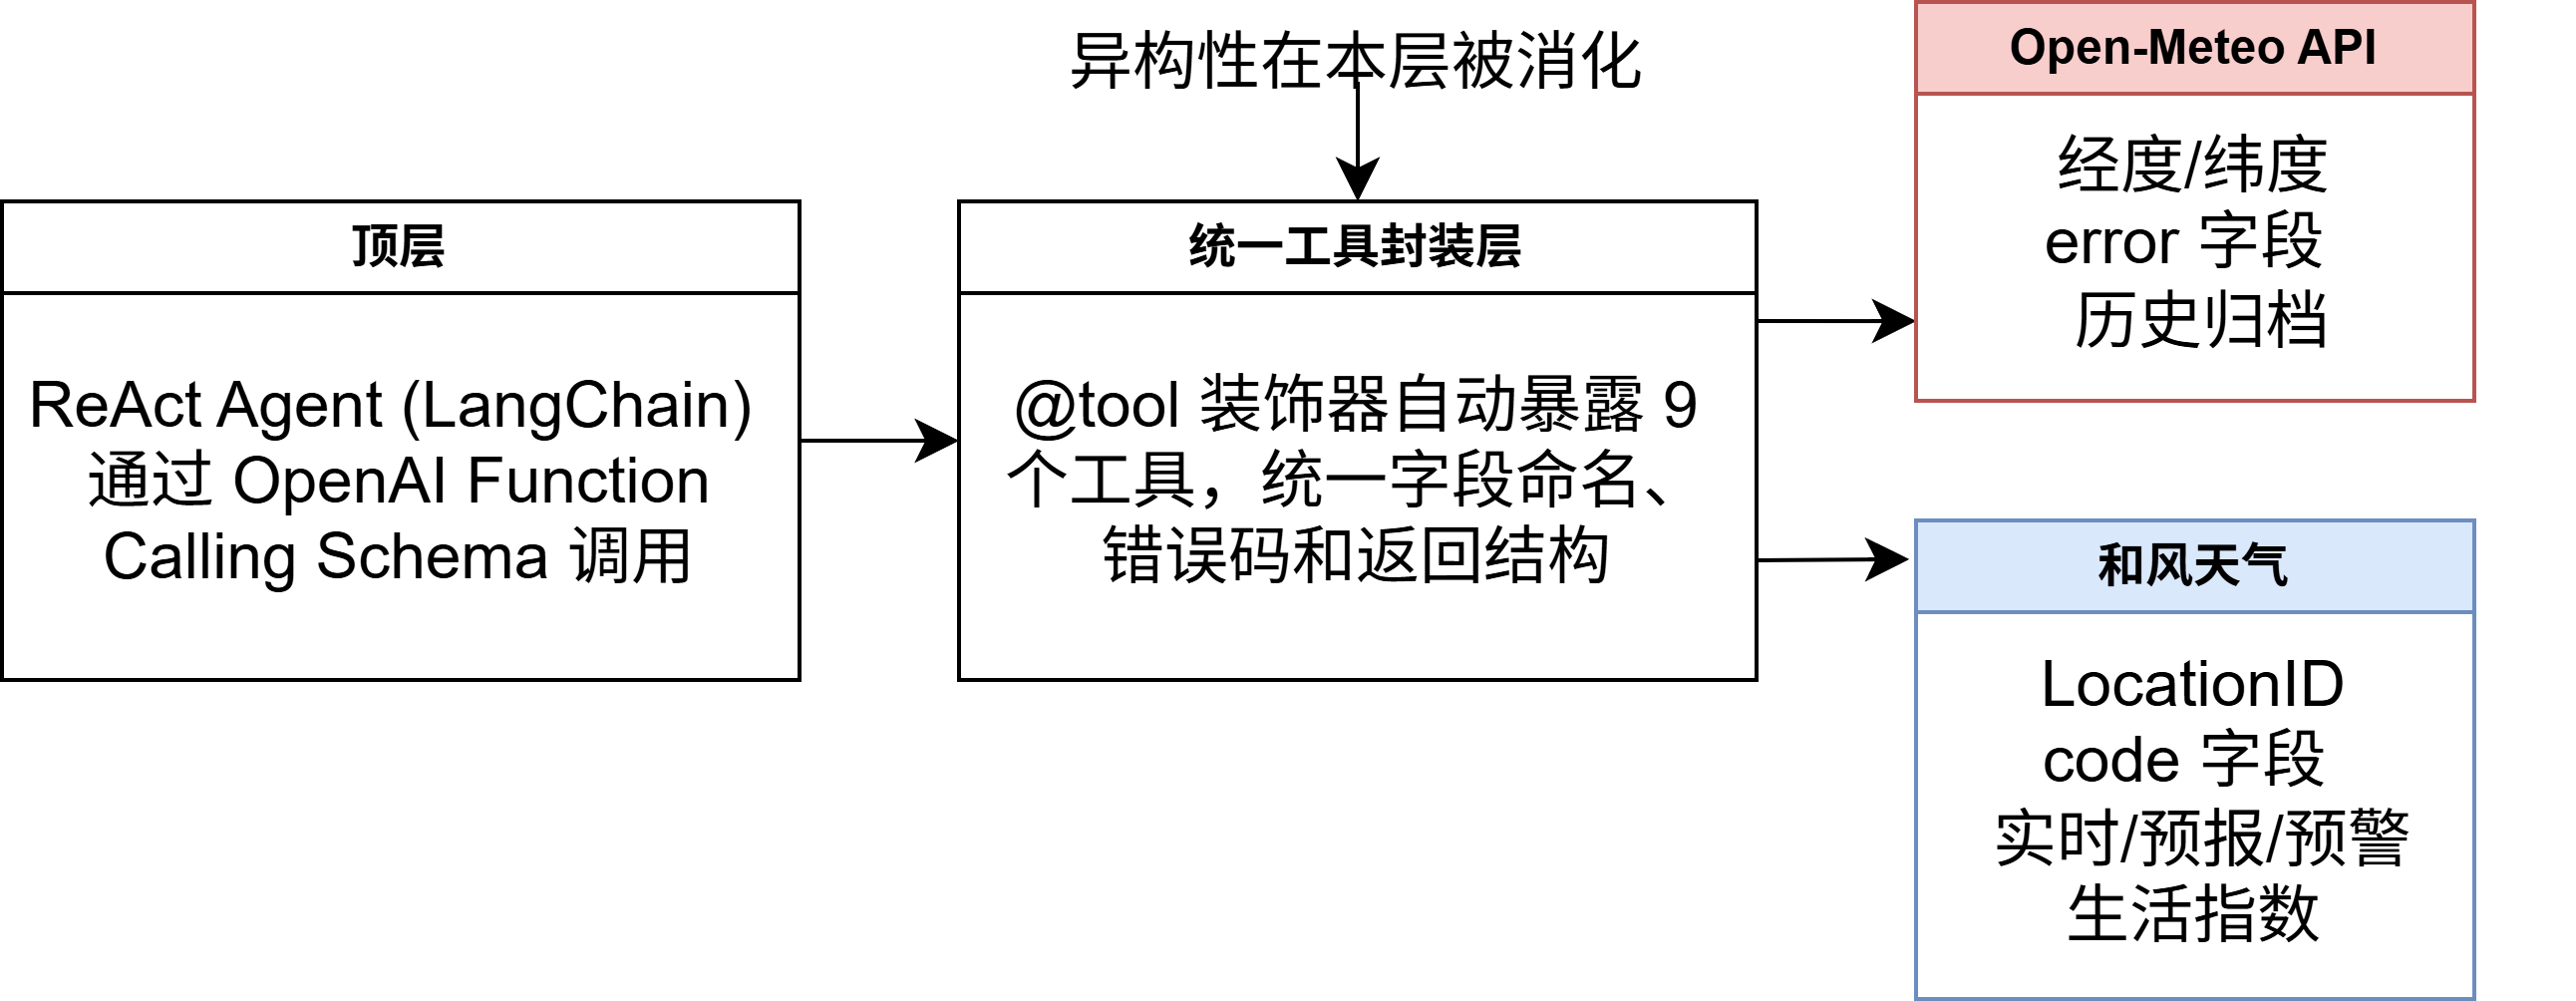
\includegraphics[width=0.92\linewidth]{figures/异构 API 统一封装层结构图}
    \caption{异构气象 API 统一封装层三层结构示意图}
    \label{fig:api-unified-wrapper}
\end{figure}

\subsubsection*{3.1.2 \quad Function Calling Schema 的设计原则}

工具暴露给大语言模型的接口规范统一遵循 OpenAI Function Calling
Schema 协议。每个工具的描述由四部分构成：函数名、
docstring 自然语言描述、参数类型注解、参数描述与可选枚举值。
LangChain 的 \texttt{@tool} 装饰器在工具被加载时自动从 Python 类型
注解与 docstring 抽取出对应的 JSON Schema，无需手工维护额外的
schema 文件。

为最大化大语言模型的工具识别准确率，本文在 docstring 编写上遵循
三条具体原则。第一条是任务驱动的功能描述。每个工具的首句直接说明
该工具解决什么问题，例如 \texttt{get\_\bk{}current\_\bk{}weather} 的首句为
获取指定地点的实时天气数据。第二条是显式的参数枚举。对于带有可选
参数的工具，docstring 中显式枚举所有合法值。例如 \texttt{get\_\bk{}forcast\_\bk{}weather}
的 \texttt{hours} 参数明确列出 24h、72h、168h 三个合法值，
\texttt{get\_\bk{}weather\_\bk{}indices} 的 \texttt{types} 参数列出 16 个
生活指数类型 ID 与对应的中文名称。第三条是显式的工具间依赖提示。
当一个工具依赖另一个工具的输出时，docstring 中明确说明这一依赖
关系，例如 \texttt{get\_\bk{}current\_\bk{}weather} 的 \texttt{location}
参数描述中明确指出 \texttt{LocationID} 可通过 \texttt{search\_\bk{}city}
获取。这一类提示是大语言模型在 ReAct 循环中正确编排多步工具调用
的关键依据，与 Patil 等 \cite{ref28} 在 Gorilla 工作中通过检索式
增强提升大语言模型对大规模 API 调用准确率的总体思路在动机上一致。

\subsubsection*{3.1.3 \quad 工具集汇总}

按上述设计原则，本文为气象 Agent 实现了 9 个 weather\_api 工具加
2 个 RAG 工具，共 11 个工具单元。其中 weather\_api 系列的 9 个工具
分为四类，详见 \reftab{tab:api-tools-overview}。RAG 类的两个工具
\texttt{search\_\bk{}knowledge} 与 \texttt{bridge\_\bk{}weather\_\bk{}data} 已在
\ref{sec:semantic-bridge} 节展开，本节不再重复。

\begin{table}[!ht]
    \centering
    \caption{气象 API 工具集汇总}
    \label{tab:api-tools-overview}
    \song\fontsize{9pt}{12pt}\selectfont
    \renewcommand{\arraystretch}{0.95}
    \begin{tabular}{lll}
        \toprule
        类别 & 工具名 & 主要功能 \\
        \midrule
        辅助 & \texttt{get\_\bk{}current\_\bk{}time} & 返回当前日期与时间，解析相对时间表达 \\
        辅助 & \texttt{search\_\bk{}city} & 城市名查 \texttt{LocationID} 与经纬度 \\
        \midrule
        实时 & \texttt{get\_\bk{}current\_\bk{}weather} & 返回观测时刻的温度、风力、降水等 \\
        预报 & \texttt{get\_\bk{}forcast\_\bk{}weather} & 24h / 72h / 168h 逐小时预报 \\
        预报 & \texttt{get\_\bk{}daily\_\bk{}forecast} & 3d / 7d / 10d / 15d / 30d 逐日预报 \\
        预警 & \texttt{get\_\bk{}weather\_\bk{}warning} & 当前生效的暴雨、台风、大风等预警 \\
        指数 & \texttt{get\_\bk{}weather\_\bk{}indices} & 1d / 3d 生活指数（16 类） \\
        \midrule
        历史 & \texttt{get\_\bk{}historical\_\bk{}hourly} & Open-Meteo 长期归档逐小时数据 \\
        历史 & \texttt{get\_\bk{}historical\_\bk{}daily} & Open-Meteo 长期归档逐日数据 \\
        \bottomrule
    \end{tabular}
\end{table}

工具集的覆盖范围与意图识别模块的 9 类意图存在明确的一对一映射关系。
\texttt{get\_\bk{}current\_\bk{}weather} 服务于 \texttt{current\_\bk{}weather} 意图，
\texttt{get\_\bk{}forcast\_\bk{}weather} 服务于 \texttt{hourly\_\bk{}forecast},
\texttt{get\_\bk{}daily\_\bk{}forecast} 服务于 \texttt{daily\_\bk{}forecast},
\texttt{get\_\bk{}weather\_\bk{}warning} 服务于 \texttt{weather\_\bk{}warning},
\texttt{get\_\bk{}weather\_\bk{}indices} 服务于 \texttt{life\_\bk{}index}，两类
\texttt{get\_\bk{}historical\_\bk{}*} 服务于历史查询，组合调用 \texttt{search\_\bk{}city}
加 \texttt{get\_\bk{}forcast\_\bk{}weather} 加 \texttt{get\_\bk{}weather\_\bk{}indices}
则服务于 \texttt{travel\_\bk{}advice} 类多地点出行场景。这一映射关系
作为推理参考写入 \texttt{INTENT\_\bk{}RECOGNIZER\_\bk{}PROMPT} 的工具映射段落，
为 \ref{sec:intent-recognition} 节的 \texttt{needed\_\bk{}tools} 字段提供
推断依据。

\subsubsection*{3.1.4 \quad 与 MCP 协议的对比与对齐}

Function Calling Schema 在工具描述层面与 Anthropic 等机构推动的 Model
Context Protocol \cite{ref11} 在设计目标上有相当部分重叠：两者都希望
通过标准化的工具接口让大语言模型与外部系统的解耦能力最大化。Function
Calling 由 OpenAI 在 GPT-4 阶段提出并被 LangChain 等主流 Agent 框架
继承，其优势是与现有大语言模型 API 紧密集成；MCP 则采用客户端服务器
架构，工具侧实现独立的 MCP Server 进程，通过 stdio 或 SSE 协议与
Agent 客户端通信，优势是在跨进程隔离与多进程编排上有更强的可扩展性。

本文选择 Function Calling 而非 MCP 的工程取舍源自三点考虑。第一是
延迟敏感性。气象 Agent 的典型响应需要在 5 至 15 秒内完成多步工具
调用与最终回答生成，跨进程通信引入的额外往返延迟在毕业设计研究
范围内不能被本课题方法论的价值充分覆盖。第二是开发与调试便利性。
\texttt{@tool} 装饰器允许工具与 Agent 共享同一份 Python 进程与
异常调用栈，调试单点工具崩溃时不需要在多进程之间检索日志。第三是
评测复用便利性。\ref{chap:evaluation} 章的 5 套评测脚本统一直接
调用同一份工具实现，避免了在评测时维护额外的 MCP 服务进程。

需要明确的是，本文工具描述格式严格遵循 OpenAI Function Calling
JSON Schema，与 MCP 工具描述格式在字段语义上一一对应。如果未来需要
迁移到 MCP 架构，仅需把 \texttt{@tool} 装饰器替换为 MCP Server 注册
逻辑，工具实现与 docstring 全部可以原样保留。这一兼容性是本文工具
封装层在工程演进路径上的一个具体保留。

% ===== END: 草稿/3_1_API封装 =====


% ===== BEGIN: 草稿/3_2_意图识别 =====
% =============================================================================
% 3.2 气象任务意图识别与指令化
% 草稿版本：v0.2 (2026-05-07)
%   v0.1：完成正文初稿。
%   v0.2：按导师意见 8 在 3.2 节首段嵌入 fig:nlu-pipeline 双阶段 NLU
%        管线图，可视化"用户问 → recognizer → completer → ReAct"
%        前置链路与两道容错回退分支。
% 字数：约 2000 字
% 风格规则：v0.2 风格（无 \textbf / \textit / 引例括号 / 双引号 / 破折号）
% 引用：\cite{ref1, ref18, ref20, ref28}
% 图表：
%   - 图 \reffig{fig:nlu-pipeline}            双阶段 NLU 前置管线图
%   - 表 \reftab{tab:intent-types}            9 类意图说明
%   - 表 \reftab{tab:weather-intent-schema}   WeatherIntent 结构化字段
% 依赖宏包：booktabs / tabularx / graphicx（主稿已加载）
% =============================================================================

\subsection{气象任务意图识别与指令化}
\label{sec:intent-recognition}

前节解决了底层 API 的工具化封装问题，但仅靠一组 Function Calling
工具仍不足以处理用户的自然语言查询。用户提问的语义
具有高度多样性，例如同样查询武汉今天的天气，用户可能说现在武汉怎么样、
武汉今天会下雨吗、明天早八到晚六从成都坐高铁到武汉有什么穿衣建议等
形态各异的句式。如果直接把原始查询送入 ReAct 循环 \cite{ref18}，
大语言模型需要同时承担意图理解、参数解析、工具选择三类任务，错误
率会显著上升。本文据此在 ReAct 循环之前增加一道独立的意图识别前置，
把自然语言查询解析为结构化 \texttt{WeatherIntent} 对象，作为
ReAct 循环的强结构化输入。整体双阶段 NLU 前置管线见
\reffig{fig:nlu-pipeline}。

\begin{figure}[!ht]
    \centering
    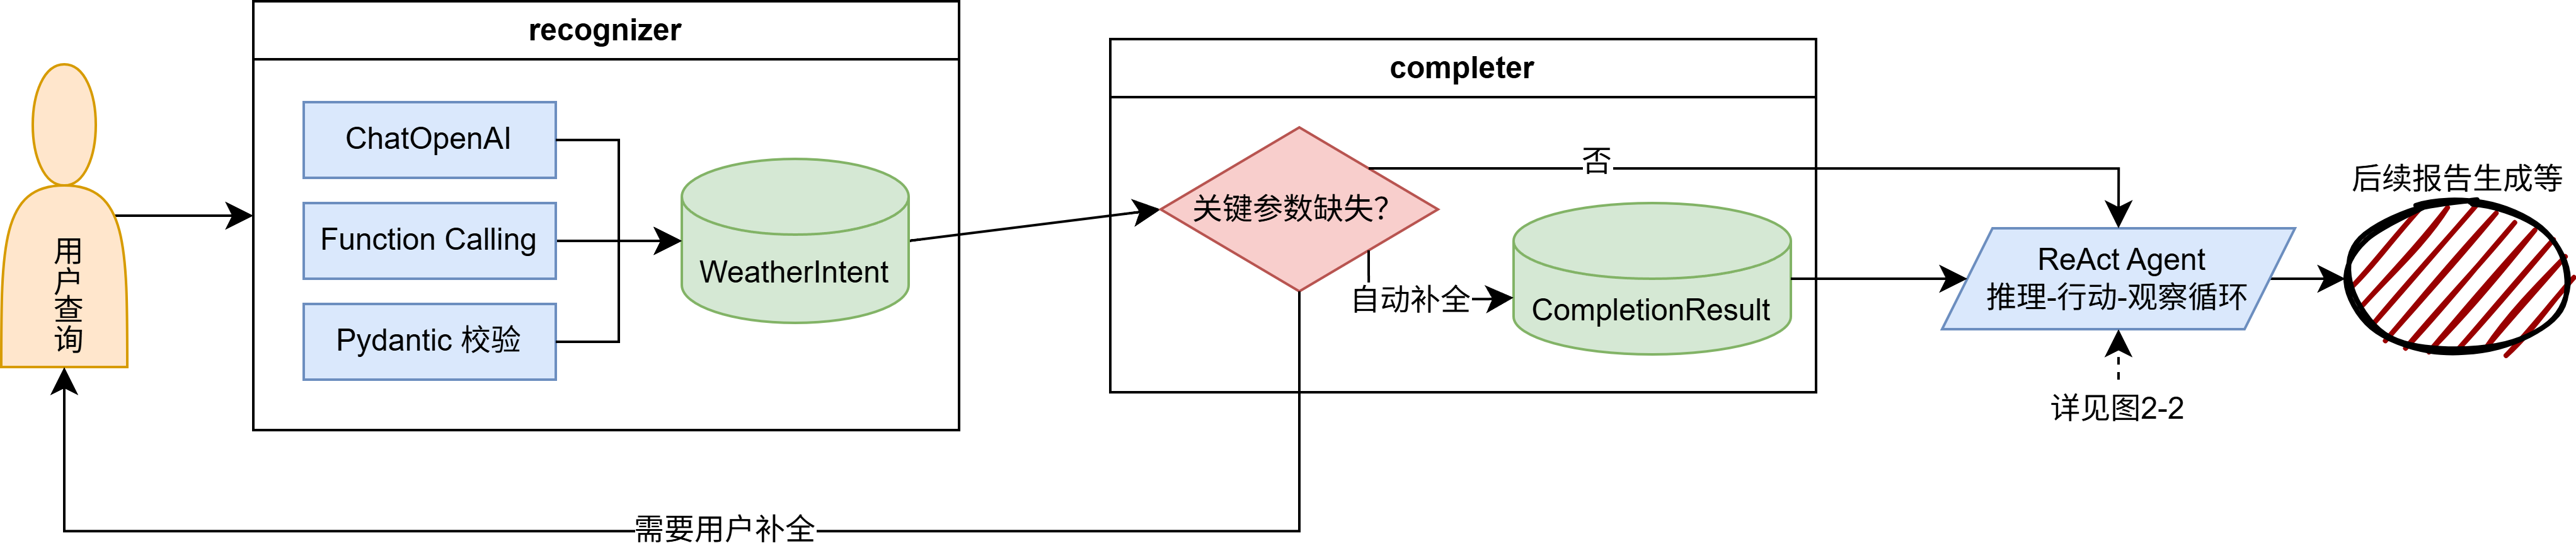
\includegraphics[width=\linewidth]{figures/双阶段 NLU 管线图 (1)}
    \caption{双阶段 NLU 前置管线示意图}
    \label{fig:nlu-pipeline}
\end{figure}

\subsubsection*{3.2.1 \quad WeatherIntent 数据模型设计}

意图识别模块的核心数据结构是 \texttt{WeatherIntent}，定义于
\texttt{src/\bk{}intent/\bk{}schema.\bk{}py}，基于 Pydantic v2 实现。该数据结构
通过 6 个关键字段刻画用户查询的全部结构化要素，详见
\reftab{tab:weather-intent-schema}。

\begin{table}[!ht]
    \centering
    \caption{WeatherIntent 数据模型字段说明}
    \label{tab:weather-intent-schema}
    \song\fontsize{9pt}{12pt}\selectfont
    \renewcommand{\arraystretch}{0.95}
    \begin{tabular}{lll}
        \toprule
        字段 & 类型 & 含义 \\
        \midrule
        \texttt{intent} & Literal\ 9 类 + unknown & 查询任务类型 \\
        \texttt{locations} & List[LocationIntent] & 涉及的所有地点及其角色 \\
        \texttt{time} & TimeIntent & 日期与起止时间 \\
        \texttt{variables} & List[str] & 关注的天气要素 \\
        \texttt{needed\_\bk{}tools} & List[str] & 建议调用的工具名 \\
        \texttt{reasoning} & Optional[str] & 意图判定的简短理由 \\
        \bottomrule
    \end{tabular}
\end{table}

子模型 \texttt{LocationIntent} 包含 \texttt{name} 与
\texttt{role} 两个字段，\texttt{role} 取 \texttt{target} 单一目标、
\texttt{departure} 出发地、\texttt{arrival} 目的地、\texttt{waypoint}
途经点四个枚举值之一。子模型 \texttt{TimeIntent} 包含 \texttt{raw\_\bk{}text}
原始时间表达、\texttt{date} 日期、\texttt{start\_\bk{}time} 起始时刻、
\texttt{end\_\bk{}time} 结束时刻四个字段，可同时承载相对时间例如明天与
绝对时间例如 2025-01-01 两类表达。\texttt{reasoning} 字段是为可调试性
专门设计的，用于让模型记录判定逻辑，便于评测阶段定位失败用例。

意图类型 \texttt{intent} 的 Literal 设计是本文降低意图识别幻觉的关键
工程手段之一。Pydantic 在结构化输出阶段会强制校验该字段必须落在
预定义的 9 类加 \texttt{unknown} 共 10 个枚举值中，若大语言模型
返回不在枚举内的值，Pydantic 会抛出 \texttt{ValidationError},
触发上游容错回退。9 类意图的具体语义见 \reftab{tab:intent-types}。

\begin{table}[!ht]
    \centering
    \caption{9 类意图类型的语义与典型查询}
    \label{tab:intent-types}
    \song\fontsize{9pt}{12pt}\selectfont
    \renewcommand{\arraystretch}{0.95}
    \begin{tabular}{lll}
        \toprule
        意图类型 & 语义 & 典型查询 \\
        \midrule
        \texttt{current\_\bk{}weather} & 当前实时天气 & 现在武汉怎么样 \\
        \texttt{hourly\_\bk{}forecast} & 逐小时预报 & 明天下午 3 点会下雨吗 \\
        \texttt{daily\_\bk{}forecast} & 逐日整体预报 & 这周武汉天气如何 \\
        \texttt{weather\_\bk{}warning} & 极端天气预警 & 上海有没有暴雨预警 \\
        \texttt{life\_\bk{}index} & 生活指数与适宜性建议 & 今天适合洗车吗 \\
        \texttt{historical\_\bk{}hourly} & 历史精细数据 & 去年这个月每小时降水 \\
        \texttt{historical\_\bk{}daily} & 历史长期数据 & 上月武汉日均最高温 \\
        \texttt{travel\_\bk{}advice} & 多地点多时段出行 & 早八到晚六从成都到武汉 \\
        \texttt{unknown} & 无法识别为以上类型 & 推荐部好看的电影 \\
        \bottomrule
    \end{tabular}
\end{table}

\subsubsection*{3.2.2 \quad recognizer 阶段的实现}

\texttt{recognizer} 模块位于 \texttt{src/\bk{}intent/\bk{}recognizer.\bk{}py}，
通过 LangChain 的 \texttt{ChatOpenAI.\bk{}with\_\bk{}structured\_\bk{}output} 接口
让大语言模型直接输出 \texttt{WeatherIntent} 对象。底层调用方式选择
\texttt{method=\bk{}"function\_\bk{}calling"} 而非 \texttt{json\_\bk{}schema}。
这一工程取舍源于 SiliconFlow 等第三方平台对 OpenAI 的
\texttt{response\_\bk{}format=\bk{}json\_\bk{}schema} 协议支持不完整，当模型规模较小
时返回的 schema 字段经常出现非法 JSON 截断，function calling 模式
通过 OpenAI 经典的 tool 调用机制返回结构化结果，兼容性最好。本文
被测模型 GLM-5.1 在 function calling 模式下的结构化输出可靠性显著
高于 \texttt{json\_\bk{}schema} 模式。

\texttt{INTENT\_\bk{}RECOGNIZER\_\bk{}PROMPT} 的具体设计包含 4 个段落。第一段
列出 9 类意图的判定语义，使用动词加典型查询的形式而非纯术语描述。
第二段列出 4 类地点角色的语义。第三段是工具映射参考，把每类意图
显式对应到 1 至 3 个工具名，引导大语言模型在 \texttt{needed\_\bk{}tools}
字段输出合理的工具调用建议。第四段是注意事项，包括仔细识别用户
提到的所有地点、准确提取时间范围、在 \texttt{reasoning} 字段简短
说明判定理由三条。这一 4 段式结构借鉴了 Hong 等 \cite{ref20} 在
Data Interpreter 中关于 prompt 模块化设计的论述，每段聚焦一类
信息类型，避免长 prompt 中的相互干扰。

\texttt{recognize\_\bk{}intent} 函数本身实现了一道单点容错回退。当
function calling 偶发返回 \texttt{None} 或抛出异常时，函数会重试
\texttt{max\_\bk{}retries=\bk{}1} 次，仍失败则返回 \texttt{intent=\bk{}"unknown"}
的兜底意图，并在 \texttt{reasoning} 字段记录失败原因。这一兜底设计
保证了下游 \texttt{completer} 与 ReAct 循环不会因为单点意图识别
故障而 crash，符合 \ref{sec:e2e-eval} 节强调的稳定性原则。

\subsubsection*{3.2.3 \quad 多地点角色识别与时空对齐}

气象任务中存在一类特殊场景。用户描述从一个地点到另一个地点的出行
计划，例如明天早八到晚六从成都到武汉。这类查询涉及 2 个或更多地点，
且每个地点对应不同的时间段。如果系统在 \texttt{locations} 字段中
仅记录地点名而不记录角色，下游 ReAct 循环会无法区分查哪一个地点
的天气、查哪一个时间段。

本文通过 \texttt{LocationIntent} 子模型的 \texttt{role} 字段显式
建模地点角色。出发地标注为 \texttt{departure}，目的地标注为
\texttt{arrival}，途经点标注为 \texttt{waypoint}，单一查询目标
默认为 \texttt{target}。在 \texttt{INTENT\_\bk{}RECOGNIZER\_\bk{}PROMPT}
的第二段中显式枚举这 4 类角色并给出语义说明，结合
\texttt{travel\_\bk{}advice} 意图类型的工具组合提示
\texttt{search\_\bk{}city + get\_\bk{}forcast\_\bk{}weather + get\_\bk{}weather\_\bk{}indices},
让大语言模型在多地点场景下学会同时输出地点名加角色二元组。

System Prompt 中的出行场景推理规则进一步把地点角色与时间段对齐。
针对早八到晚六从 A 到 B 的典型表述，规则约定：出发时间段查 A 地
的天气，到达时间段查 B 地的天气，不查 A 地晚上或 B 地早上的天气，
因为用户那时不在那里。这一规则的工程意义是把意图层的多角色标注
传递到 Agent 层的具体工具调用上，避免出现查了无关时段地点的天气
而消耗工具调用额度的问题。

\ref{sec:intent-eval} 节的评测结果验证了这一设计的有效性。在
\texttt{travel\_\bk{}advice} 类 5 条用例上 \texttt{location\_\bk{}role\_\bk{}accuracy}
达到 100\%，包含 \texttt{departure}、\texttt{arrival}、
\texttt{waypoint} 三类角色的复杂用例例如从西安自驾到敦煌途经张掖
也全部正确识别。这一结果表明显式枚举地点角色加 few-shot 提示能够
把大语言模型在命名实体识别加关系抽取上的能力从模糊识别提升到精确
角色标注，与 Kim 等 \cite{ref1} 在 ClimateAgent 中关于多 agent
角色专门化的论述在工程形态上同源但在实现上更加轻量。

\subsubsection*{3.2.4 \quad 对抗鲁棒性的工程处理}

意图识别还需要处理与气象无关的查询。例如推荐部好看的电影、我想看
电影等用户输入虽然语法上合法，但语义上与气象查询无关。如果
\texttt{recognizer} 强行把这类查询解析为某个气象意图，下游会触发
不必要的工具调用并返回不相关的结果。

本文通过 \texttt{intent=\bk{}"unknown"} 兜底意图与 \texttt{INTENT\_\bk{}RECOGNIZER\_\bk{}PROMPT}
中的对抗鲁棒提示共同处理这类场景。当 \texttt{recognizer} 输出
\texttt{unknown} 时，下游 \texttt{completer} 会判定 \texttt{is\_\bk{}complete=\bk{}False}
并返回友好追问，让用户在气象查询语义下重述问题。
\ref{sec:intent-eval} 节的评测中
\texttt{adversarial} 类 2 条用例端到端通过率为 100\%，验证了这一
兜底机制的可用性。

% ===== END: 草稿/3_2_意图识别 =====


% ===== BEGIN: 草稿/3_3_参数补全 =====
% =============================================================================
% 3.3 缺失检索参数的上下文推理与动态补全
% 草稿版本：v0.2 (2026-05-07)
%   v0.1：完成正文初稿。
%   v0.2：按导师意见 8 在 3.3.3 末段嵌入 fig:completion-three-tier
%        三档补全策略流程图，可视化"默认值 → 上下文推断 → 常识"
%        优先级链与失败时触发 follow_up_question 的兜底分支。
% 字数：约 1700 字
% 风格规则：v0.2 风格（无 \textbf / \textit / 引例括号 / 双引号 / 破折号）
% 引用：\cite{ref10, ref15, ref29}
% 图表：
%   - 图 \reffig{fig:completion-three-tier}         三档补全策略流程图
%   - 表 \reftab{tab:completion-required-params}    各意图类型的关键参数清单
%   - 表 \reftab{tab:completion-sources}            四类补全来源
% 依赖宏包：booktabs / tabularx / graphicx（主稿已加载）
% =============================================================================

\subsection{缺失检索参数的上下文推理与动态补全}
\label{sec:param-completion}

前节的 \texttt{recognizer} 解决了把自然语言查询解析为结构化意图的
问题，但实际查询中用户经常省略关键参数。
例如查明天天气怎么样省略了地点、查武汉怎么样省略了时间、查现在适合
洗车吗省略了城市。如果系统直接把这类不完整意图送入 ReAct 循环，会
触发两类失败：一类是模型自行编造缺失参数，例如把缺地点的查询补成
当前位置等虚构城市；另一类是模型按某个默认值兜底但不告诉用户，导致
用户得到与预期不符的回答。本文据此设计了独立的参数补全模块
\texttt{completer}，位于 \texttt{src/\bk{}intent/\bk{}completer.\bk{}py}，承担缺失
参数判定、自动补全、与友好追问三类职责。

\subsubsection*{3.3.1 \quad 分层架构的设计动机}

参数补全在工程上完全可以与意图识别合并到同一个大语言模型调用中
完成，但本文选择把两者切分为独立的两阶段管线，理由源自单点错误
的容错性考虑 \cite{ref10}。意图识别与参数补全在错误模式上具有
不同的特征：意图识别错误通常是分类边界模糊，例如把
\texttt{daily\_\bk{}forecast} 误判为 \texttt{hourly\_\bk{}forecast}；参数
补全错误则通常是字段填充幻觉，例如把没有提及地点的查询补出虚构
城市。两类错误若混合在同一次大语言模型调用中，模型在生成
\texttt{intent} 字段时的注意力分配会与生成 \texttt{locations}
字段时相互干扰。

分层架构允许后置阶段在前置阶段产生抖动时进行业务层兜底。
\ref{sec:intent-eval} 节的 \texttt{index\_\bk{}004\_\bk{}no\_\bk{}loc} 用例提供了
这一容错机制的具体实证。该用例的查询是今天去爬山合适吗，
\texttt{recognizer} 输出 \texttt{intent=\bk{}life\_\bk{}index} 正确判定意图，
但在 \texttt{locations} 字段填入了虚构的当前位置作为礼貌性补白。
\texttt{completer} 阶段识别出当前位置不是合法城市名，触发
\texttt{is\_\bk{}complete=\bk{}False} 与友好追问，最终系统反问用户希望查询
哪个城市。如果不分层，单次大语言模型调用产生地点幻觉后会直接
进入 ReAct 循环并去查虚构城市的生活指数，业务层无从纠正。
这一案例印证了分层架构本身即是容错机制，与 ChatDev \cite{ref29}
中按软件工程瀑布模型把开发任务分阶段交由不同角色协作以减少幻觉
的总体思路在精神上接近。

\subsubsection*{3.3.2 \quad 关键参数清单与判定逻辑}

\texttt{completer} 模块通过显式列出每类意图的关键参数清单来实现
缺失判定，详见 \reftab{tab:completion-required-params}。各意图
类型对参数完整性的要求差异显著：\texttt{current\_\bk{}weather} 仅要求
有地点不要求有时间，因为实时天气默认查当前；
\texttt{travel\_\bk{}advice} 要求至少 2 个地点加完整时间，因为出行场景
本质上是多地点多时段的复合查询。

\begin{table}[!ht]
    \centering
    \caption{各意图类型的关键参数清单}
    \label{tab:completion-required-params}
    \song\fontsize{9pt}{12pt}\selectfont
    \renewcommand{\arraystretch}{0.95}
    \begin{tabular}{ll}
        \toprule
        意图类型 & 关键参数 \\
        \midrule
        \texttt{current\_\bk{}weather} & \texttt{locations} \\
        \texttt{hourly\_\bk{}forecast} & \texttt{locations} + \texttt{time.\bk{}date} \\
        \texttt{daily\_\bk{}forecast} & \texttt{locations} + \texttt{time.\bk{}date} \\
        \texttt{weather\_\bk{}warning} & \texttt{locations} \\
        \texttt{life\_\bk{}index} & \texttt{locations} + \texttt{time.\bk{}date} \\
        \texttt{historical\_\bk{}hourly} & \texttt{locations} + \texttt{time.\bk{}date} 起止日期 \\
        \texttt{historical\_\bk{}daily} & \texttt{locations} + \texttt{time.\bk{}date} 起止日期 \\
        \texttt{travel\_\bk{}advice} & 至少 2 个 \texttt{locations} + \texttt{time} \\
        \bottomrule
    \end{tabular}
\end{table}

\texttt{completer} 把关键参数清单写入 \texttt{COMPLETER\_\bk{}PROMPT}
的结构化系统提示中，以列表形式让大语言模型在每次判定时显式对照。
这一显式枚举的设计避免了模型自行猜测哪些字段是关键的不确定性。
当某个关键参数缺失且无法自动补全时，模型输出
\texttt{is\_\bk{}complete=\bk{}False} 并填写 \texttt{follow\_\bk{}up\_\bk{}question}
字段，例如您想查询哪个城市的生活指数。

\subsubsection*{3.3.3 \quad 三档补全策略与四类补全来源}

对于可推断的缺失参数，\texttt{completer} 使用三档优先级补全策略。
第一档是默认值规则。当用户未指明时间但意图允许时，默认补
\texttt{time.\bk{}date} 等于今天。这一档处理日常查询省略时间的常见
情形。第二档是上下文推断。模块在调用时可选传入
\texttt{conversation\_\bk{}context} 参数，承载历史对话摘要。基于历史
对话推断的典型场景包括用户上一轮问过北京，本轮问那明天呢应补
\texttt{location=\bk{}北京}。第三档是常识推断。例如用户说早上而未指明
具体时刻，模块按行业惯例补 \texttt{start\_\bk{}time=\bk{}06:00}, 
\texttt{end\_\bk{}time=\bk{}09:00}。三档之间的优先级关系是：用户输入优于
上下文推断、上下文推断优于默认值、默认值优于常识推断，避免补全
之间相互覆盖。

每条补全操作都会被写入 \texttt{CompletionResult.\bk{}notes} 字段。
单条记录由 \texttt{field}、\texttt{value}、\texttt{source}、
\texttt{reason} 四个子字段组成。其中 \texttt{source} 取四个枚举值
之一，详见 \reftab{tab:completion-sources}。

\begin{table}[!ht]
    \centering
    \caption{补全记录的四类来源}
    \label{tab:completion-sources}
    \song\fontsize{9pt}{12pt}\selectfont
    \renewcommand{\arraystretch}{0.95}
    \begin{tabular}{ll}
        \toprule
        来源 & 含义 \\
        \midrule
        \texttt{user\_\bk{}input} & 用户在原始查询中明确给出 \\
        \texttt{context\_\bk{}inference} & 从历史对话或前置上下文推断 \\
        \texttt{default} & 使用合理默认值，例如时间默认今天 \\
        \texttt{common\_\bk{}sense} & 基于行业惯例或日常常识推断 \\
        \bottomrule
    \end{tabular}
\end{table}

四类来源在用户体验上的差异是关键工程考虑。\texttt{user\_\bk{}input} 不
需要向用户解释；\texttt{default} 与 \texttt{common\_\bk{}sense} 需要在
最终回答中告知用户系统采用了什么默认值，便于用户在系统理解错误
时纠正；\texttt{context\_\bk{}inference} 需要让用户了解系统是从上下文
推断的。\texttt{format\_\bk{}completion\_\bk{}notes} 函数把 notes 列表
格式化为人类可读文本，注入到 ReAct Agent 的首条用户消息中，最终
报告生成阶段会以参数补全说明的形式向用户展示。三档补全的判定与
回退路径整体形态见 \reffig{fig:completion-three-tier}。

\begin{figure}[!ht]
    \centering
    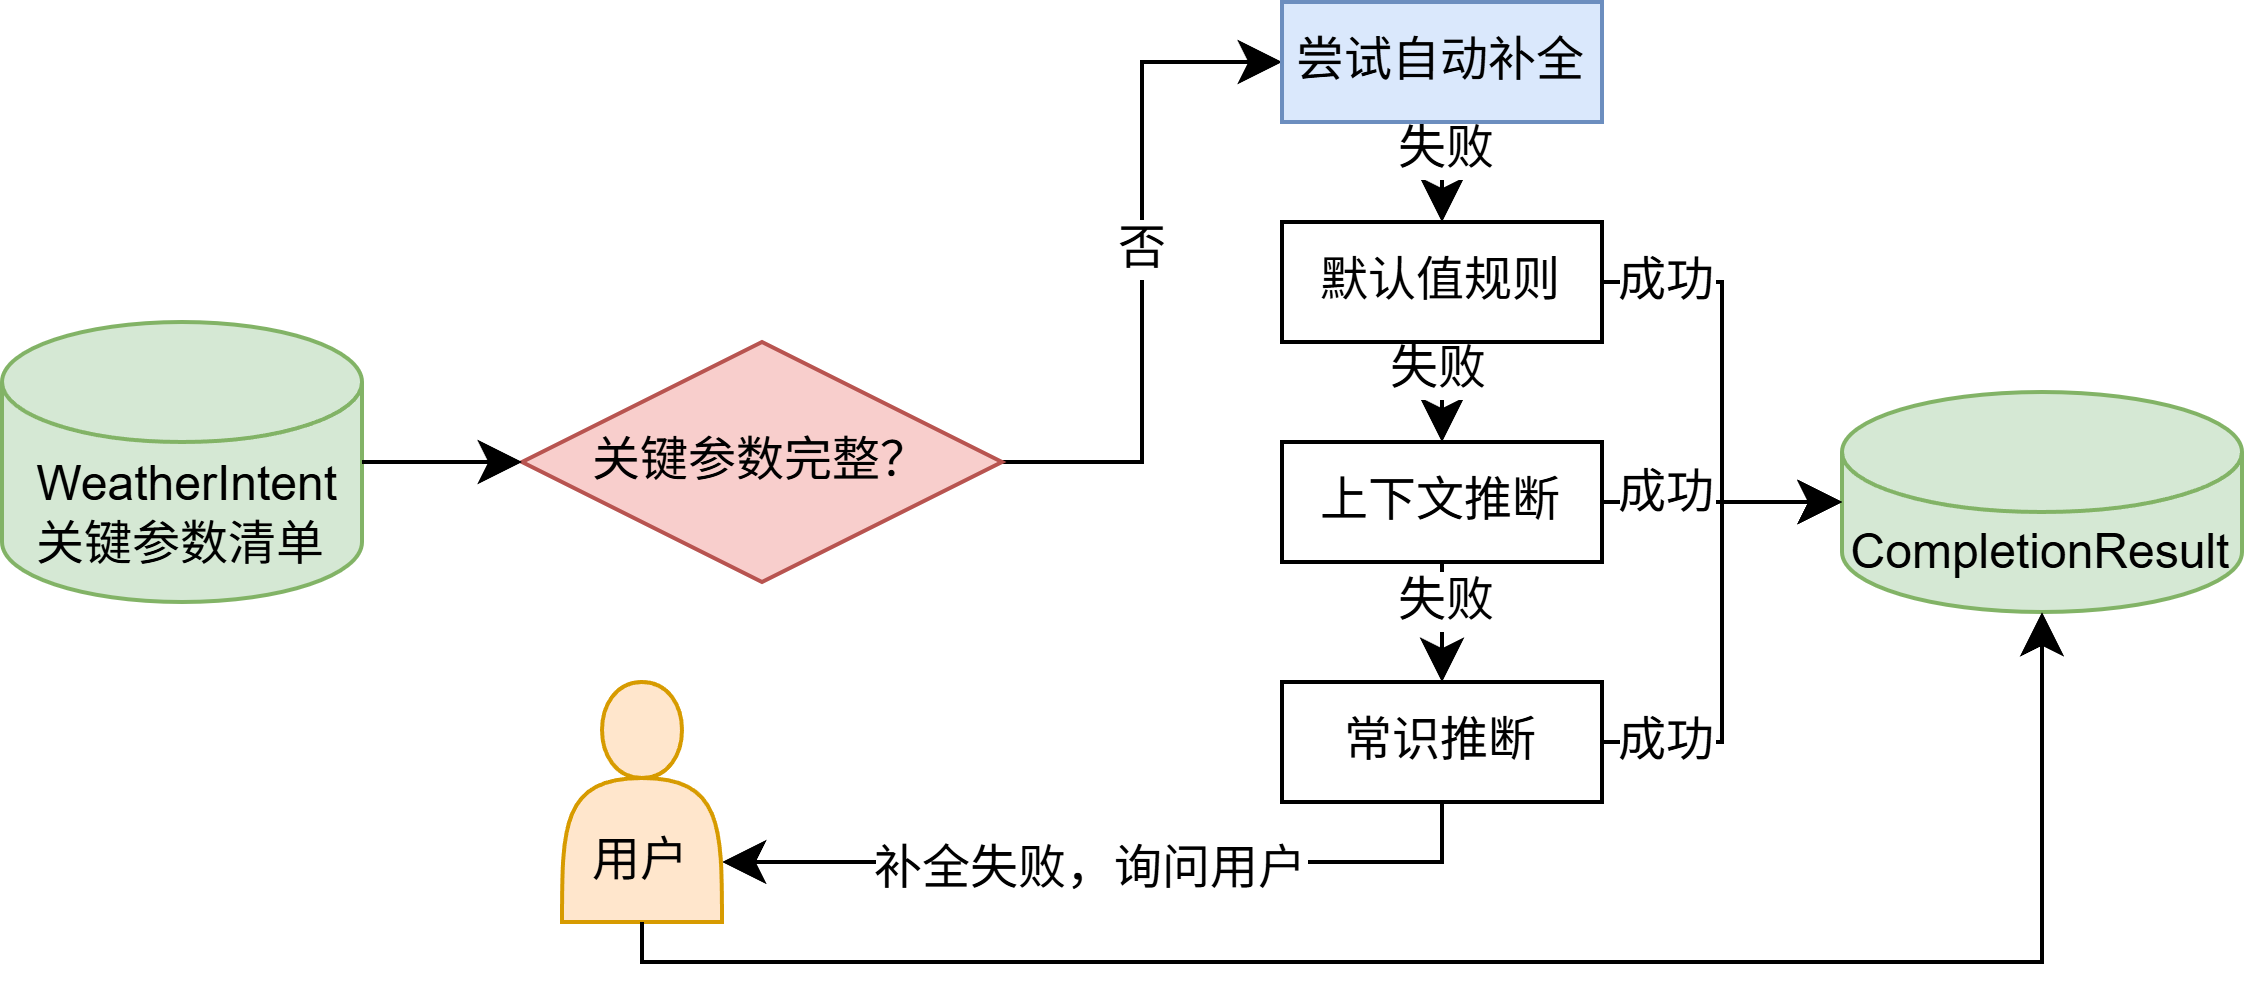
\includegraphics[width=0.78\linewidth]{figures/三档补全策略流程图}
    \caption{三档补全策略流程示意图}
    \label{fig:completion-three-tier}
\end{figure}

\subsubsection*{3.3.4 \quad 容错回退与可观测性}

\texttt{complete\_\bk{}intent} 函数同样实现了与 \texttt{recognize\_\bk{}intent}
对称的容错回退。当结构化输出多次返回 \texttt{None} 或抛出异常时，
函数返回 \texttt{is\_\bk{}complete=\bk{}True} 加原意图原样透传的兜底结果，
让 ReAct 循环可以继续推进，避免在意图理解前置就因偶发故障而
中止整个对话。这一兜底策略的代价是该次查询将放弃参数补全的
可解释性，但保证了系统级可用性。

可观测性是分层架构的另一项工程价值。每次 \texttt{recognize\_\bk{}intent}
与 \texttt{complete\_\bk{}intent} 的输入输出在 \texttt{run\_\bk{}agent} 函数
中以独立段落打印到日志，便于评测与生产排障时定位失败究竟发生在
哪一阶段。LangChain 框架 \cite{ref15} 提供的 \texttt{create\_\bk{}agent}
接口允许 ReAct 循环本身的中间状态以 stream 模式实时输出，与
意图识别加补全两阶段日志合并形成 4 阶段可追溯链条：原始查询、
\texttt{WeatherIntent}、\texttt{CompletionResult}、ReAct 工具
调用与最终回答。这一链条在
\ref{sec:e2e-eval} 节端到端评测中被进一步利用，作为
\texttt{e2e\_\bk{}intent\_\bk{}cache} 与 \texttt{e2e\_\bk{}agent\_\bk{}cache} 两层
缓存的天然切分点。

% ===== END: 草稿/3_3_参数补全 =====


% ===== BEGIN: 草稿/3_4_本章小结 =====
% =============================================================================
% 3.4 本章小结
% 草稿版本：v0.1 (2026-05-05)
% 字数：约 500 字
% 风格规则：v0.2 风格（无 \textbf / \textit / 引例括号 / 双引号 / 破折号）
% 依赖宏包：booktabs / tabularx（主稿已加载）
% =============================================================================

\subsection{本章小结}
\label{sec:retrieval-summary}

本章针对开题报告中提出的气象任务指令解析问题，从工具学习与意图
理解两个维度构建了从自然语言查询到结构化检索请求的完整链路。

\ref{sec:api-tooling} 节解决了底层异构 API 的统一接入与工具化封装。
本文同时接入和风天气与 Open-Meteo 两类异构数据源，覆盖实时观测、
预报、预警、生活指数与长期历史归档五类业务场景，并通过 LangChain
\texttt{@tool} 装饰器把 9 个 weather\_api 工具加 2 个 RAG 工具
统一封装为符合 OpenAI Function Calling Schema 协议的工具单元。
docstring 编写遵循任务驱动描述、显式枚举可选参数、显式工具间依赖
提示三条原则，最大化大语言模型的工具识别准确率。Function Calling
与 Model Context Protocol 在工具描述格式上一一对应，本文工具封装
保留了未来迁移到 MCP 架构的兼容性。

\ref{sec:intent-recognition} 节解决了从自然语言到结构化意图的
转化。本文设计了 \texttt{WeatherIntent} 数据模型，通过 6 个字段
刻画意图类型、地点角色、时间范围、关注要素、建议工具、判定理由。
\texttt{recognizer} 模块基于 \texttt{ChatOpenAI.\bk{}with\_\bk{}structured\_\bk{}output}
的 function calling 模式实现结构化输出，9 类意图通过 Pydantic
Literal 强制校验，避免分类幻觉。多地点角色识别通过显式枚举 4 类
角色加 few-shot 提示在 \texttt{travel\_\bk{}advice} 类用例上达到 100\%
准确率。\texttt{intent=\bk{}"unknown"} 兜底意图加 \texttt{adversarial}
对抗鲁棒提示共同处理与气象无关的查询。

\ref{sec:param-completion} 节解决了缺失参数的上下文推理与动态补全。
独立的 \texttt{completer} 模块以分层架构吸收 \texttt{recognizer}
阶段的字段级幻觉，通过 \texttt{is\_\bk{}complete}、\texttt{follow\_\bk{}up\_\bk{}question}、
\texttt{notes} 三字段语义实现可推断字段的自动补全与不可推断字段
的友好追问。三档补全策略与四类补全来源把每条补全操作显式记录在
\texttt{notes} 字段，最终在报告生成阶段向用户透明展示。

本章工作的实证验证将在 \ref{sec:intent-eval} 节展开。35 条 10 类
评测集上端到端通过率 91.4\%、地点角色准确率 100\%、单轮 8 类场景
全部 100\% 通过的结果共同验证了本章方法的有效性。下一章在本章
结构化检索基础上展开异构数据语义化与数值幻觉两个研究问题对应的
语义桥接与统计分析方法。

% ===== END: 草稿/3_4_本章小结 =====



\sectionbreak

\section{融合语义桥接机制的气象数据统计分析方法}
\label{chap:semantic-bridge}

% ===== BEGIN: 草稿/4_1_语义桥接 =====
% =============================================================================
% 4.1 气象"数据-文本"语义桥接算法
% 草稿版本：v0.4 (2026-05-07)
%   v0.2：按写作风格规则去除 \textbf / \textit 与括号"如..."句式。
%   v0.3：嵌入 1 张图与 3 张表，由对应 \reffig / \reftab 引用就近浮动。
%   v0.4：按导师反馈第 12 条新增"桥接前后模型上下文对比图"
%        （fig:bridge-context-compare）。考虑到对比内容核心是 ASCII 化的
%        工具调用 JSON 与决策文本，弃用 drawio，改用 minipage + \ttfamily
%        \scriptsize + \fbox 直接在 LaTeX 中以左右两栏代码块形式排版。
% 字数：约 1800 字（不含图表 caption）
% 引用：\cite{ref2, ref5, ref10, ref12, ref20, ref22, ref24}
% 图表：
%   - 图 \reffig{fig:dual-path-rag}            双通路 RAG 架构示意图
%   - 图 \reffig{fig:bridge-context-compare}   桥接前后模型上下文对比（双栏代码）
%   - 表 \reftab{tab:rag-weight-sweep}         60 条 × 8 个权重点扫描结果
%   - 表 \reftab{tab:semantic-mapping}         5 类要素分级阈值映射节选
%   - 表 \reftab{tab:bridge-ablation}          通路 B 四档消融总表（71 条）
% 依赖宏包：booktabs / tabularx / siunitx / graphicx（主稿已加载）
% =============================================================================

\subsection{气象"数据-文本"语义桥接算法}
\label{sec:semantic-bridge}

气象预报数据的智能分析面临一个核心矛盾。原始数据以高度结构化的数值形式
存在，例如 24 小时累积降水量 $\SI{52.3}{mm}$、$10\,\mathrm{m}$ 风速
$\SI{14.1}{m/s}$；而用户的决策语义却以自然语言形式表达，例如暴雨警示或
大风影响出行。直接把数值丢给大语言模型让其自由生成解读文本存在严重的
幻觉风险。一方面，大语言模型无法稳定输出与国家标准一致的等级编号；
另一方面，大语言模型倾向于凭训练语料的印象编造引用源
\cite{ref10, ref20}。本节针对这一问题提出双通路检索增强生成（Dual-Path
Retrieval-Augmented Generation, Dual-Path RAG）架构，把数值到语义的转换
任务从大语言模型的自由发挥改为基于确定性分级器与混合检索的预处理与引用
闭环，从根本上规避数值理解阶段的幻觉。

\subsubsection*{4.1.1 \quad 双通路 RAG 架构概览}

借鉴 Lewis 等 \cite{ref12} 提出的 RAG 框架与 Gao 等 \cite{ref24} 综述
中的混合检索思想，本文将知识检索分解为两条互补的通路，整体结构如
\reffig{fig:dual-path-rag} 所示。

\begin{figure}[!ht]
    \centering
    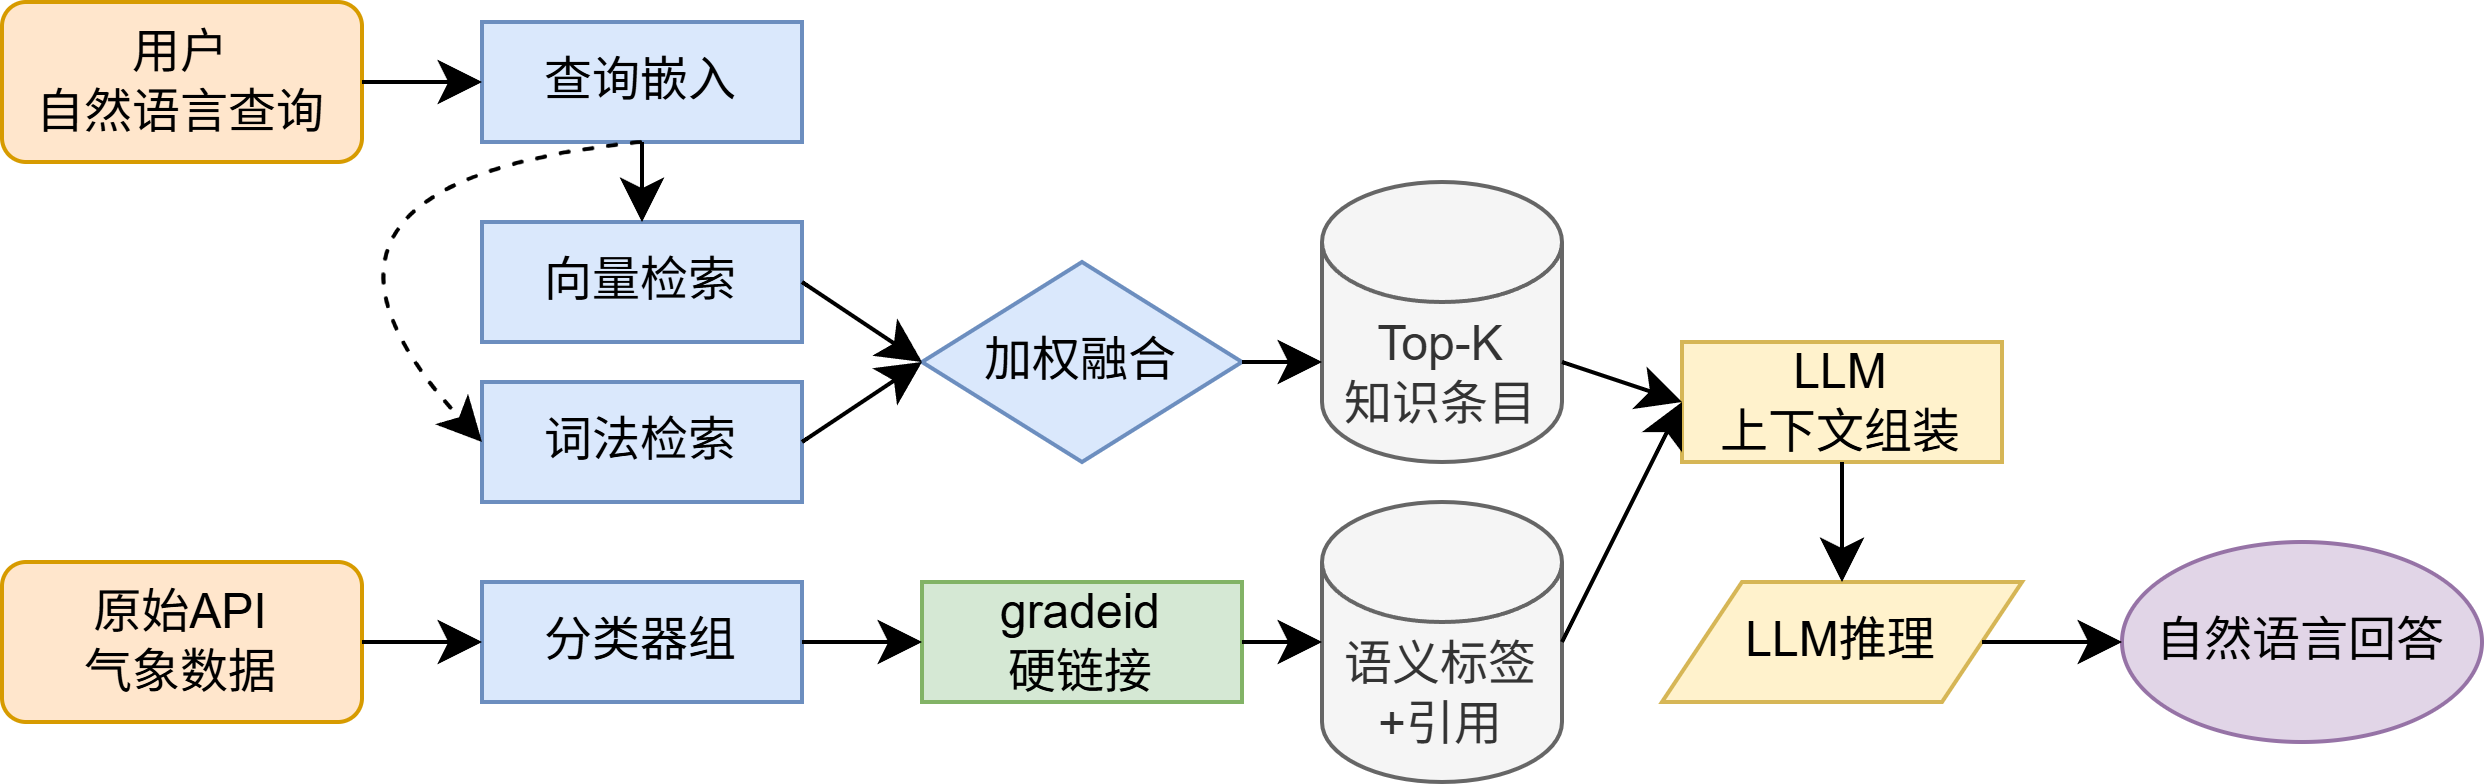
\includegraphics[width=0.95\linewidth]{figures/dual_path_rag}
    \caption{双通路 RAG 架构示意图}
    \label{fig:dual-path-rag}
\end{figure}

通路 A 承担混合语义检索任务，面向概念、操作、改写类自然语言查询。
该通路采用向量检索 (BAAI/bge-m3) 与 BM25 词法检索的加权融合，从
向量化知识库中召回 Top-$K$ 条相关条目，作为大语言模型生成自然
语言回答的上下文，典型查询例如什么是雷暴、几级风必须停止高空作业
等。

通路 B 承担确定性分级与硬链接式语义桥接任务，面向数值到等级再到
标准引用类需求。该通路由一组按要素分别实现的确定性分类器完成阈值
判定，通过 \texttt{grade\_\bk{}id} 字段硬链接到知识库的对应条目，由
富化器一次性返回语义标签、影响描述与引用源三元组，典型任务例如把
$\SI{52.3}{mm}$ 判为暴雨并附上 GB/T 28592-2012 的具体条款。

两条通路的设计动机可以从两类查询的本质差异得到解释。通路 A 面对的
是召回问题，只要知识库内包含相关条目，混合检索就能以高 Recall 召回；
通路 B 面对的是精确归属问题，任意嵌入模型在小型知识库上都难以保证
相邻阈值条目的 Top-1 排序正确性，例如大暴雨 $100\sim249.9\,\mathrm{mm}$
与特大暴雨 $\geq 250\,\mathrm{mm}$ 在向量空间中往往邻近，因此必须由
确定性规则承担最终归属判定。两条通路共同覆盖了异构数据语义化与
数值理解幻觉两个研究问题 \cite{ref2, ref5}，在功能上互不重叠并
共同覆盖检索路径的两端。

\subsubsection*{4.1.2 \quad 通路 A 混合语义检索的设计与权重消融}

通路 A 的核心是把向量距离与词法相关性以可调权重组合：

\begin{equation}
    \mathrm{Score}_{\mathrm{hybrid}}(q, d) =
        \alpha \cdot \mathrm{Sim}_{\mathrm{vec}}(q, d) +
        (1 - \alpha) \cdot \mathrm{Score}_{\mathrm{BM25}}(q, d)
\end{equation}

其中 $\alpha$ 为向量权重，$1 - \alpha$ 为 BM25 权重，二者归一化后线性
融合。本文在 60 条覆盖 8 类查询的检索评测集上系统扫描了 $\alpha \in
\{0.0, 0.5, 0.7, 0.8, 0.85, 0.9, 0.95, 1.0\}$ 共 8 个权重点,详见
\reftab{tab:rag-weight-sweep}，得到三条工程结论。

\begin{table}[!ht]
    \centering
    \caption{通路 A 混合检索权重扫描}
    \label{tab:rag-weight-sweep}
    \song\wuhao
    \begin{tabular}{cccccc}
        \toprule
        $\alpha$（向量权重） & $1-\alpha$（BM25 权重） & Top-1 & MRR & Recall@1 & Recall@5 \\
        \midrule
        0.00 & 1.00 & 81.7\% & 0.872 & 73.3\% & 91.7\% \\
        0.50 & 0.50 & 78.3\% & 0.851 & 70.0\% & 96.7\% \\
        0.70 & 0.30 & 80.0\% & 0.864 & 71.7\% & 96.7\% \\
        0.80 & 0.20 & 81.7\% & 0.872 & 73.3\% & 96.7\% \\
        0.85 & 0.15 & 83.3\% & 0.892 & 75.0\% & 97.7\% \\
        0.90 & 0.10 & 85.0\% & 0.908 & 76.7\% & 97.7\% \\
        0.95 & 0.05 & 85.0\% & 0.908 & 76.7\% & 97.7\% \\
        1.00 & 0.00 & 81.7\% & 0.872 & 73.3\% & 96.7\% \\
        \bottomrule
    \end{tabular}
\end{table}

第一，混合检索的边际增益是真实存在的。当 $\alpha$ 取最优值 0.9 时，
Top-1 命中率达到 85.0\%，平均倒数排名达到 0.908，分别比纯向量
($\alpha = 1.0$) 高出 3.3 个百分点与 0.036，比纯 BM25 ($\alpha = 0.0$)
同样高出 3.3 个百分点与 0.036。这表明向量检索擅长概念性查询，BM25 擅长
数值阈值字面匹配，二者优势正交，需要融合。

第二，最优权重随知识库体量动态漂移。在初版 44 条知识库与 43 条评测集上
最优 $\alpha = 0.80$；在扩展到 62 条知识库与 60 条评测集之后，最优值
上调至 0.90。这一现象的原因是知识库扩大后相邻条目的语义距离变近，
BM25 词法噪声在小权重下反而成为干扰。该结论为工程实践提供了一条可推广
的指导原则：混合检索的权重不能一次调好用到底，应随知识库规模重新校准。

第三，通路 A 的盲区暴露了通路 B 的必要性。即使在最优权重下，仍有
约 9.3\% 的 Top-1 脱靶用例，且全部集中在数值阈值与术语别名类查询。
例如 query 降水 $\SI{200}{mm}$ 算什么级别应命中大暴雨
$100\sim249.9\,\mathrm{mm}$，实际却被错误排到特大暴雨 $\geq 250\,
\mathrm{mm}$；query 强风是几级风由于强风既是蒲福 6 级专名又是台风条目
高频词，被混合检索召回到了 \texttt{term\_\bk{}typhoon} 条目。这一类失败靠
任何嵌入模型在小型知识库上都难以彻底解决，从而构成了通路 B 即确定性
分级器的工程必要性。

\subsubsection*{4.1.3 \quad 通路 B 确定性分级器与硬链接式语义桥接}

通路 B 的实现思路源自 Gruver 等 \cite{ref22} 关于大语言模型在精确数值
任务上表现局限性的实证。在数值到等级映射这一确定性可枚举的任务上，让
大语言模型自由发挥反而引入幻觉，正确做法是把规则显式编码为
\texttt{if/\bk{}elif} 函数。通路 B 内部的数据流形态见
\reffig{fig:path-b-internal}：原始数值经由确定性分级器判定等级后，
通过 \texttt{grade\_\bk{}id} 字段直接硬链接到知识库的对应条目，由富化器
一次性返回带引用源的语义标签三元组，全程绕过向量检索的排序不确定性。

\begin{figure}[!ht]
    \centering
    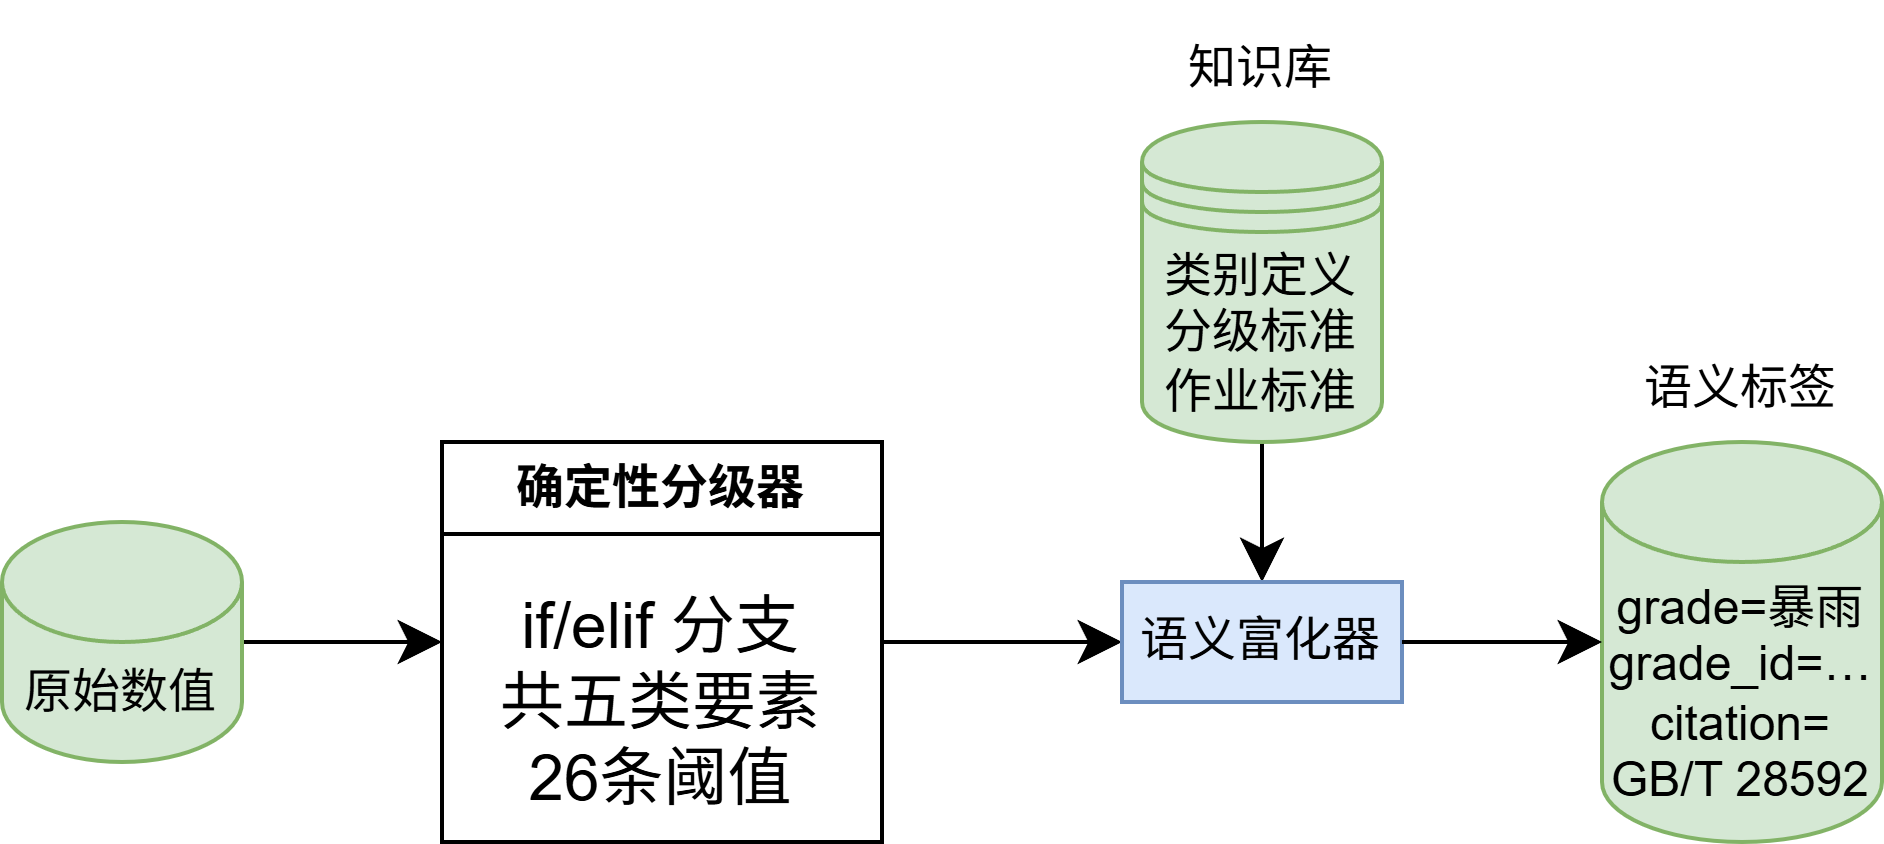
\includegraphics[width=\linewidth]{figures/通路 B 内部数据流图}
    \caption{通路 B 内部数据流示意图}
    \label{fig:path-b-internal}
\end{figure}

本文为五类典型气象要素实现了独立分类器，分别
处理降水量、风速、温度、能见度与相对湿度。每个分类器返回
\texttt{SemanticLabel} 对象，包含三个关键字段。\texttt{grade} 是语义
等级名，例如暴雨、疾风、高温酷热。\texttt{grade\_\bk{}id} 是与知识库条目
唯一对应的硬链接 ID，例如 \texttt{grading\_\bk{}precipitation\_\bk{}24h\_\bk{}rainstorm}，
用于通过 \texttt{KnowledgeBase.\bk{}get\_\bk{}by\_\bk{}id} 直接查表，避免向量检索的
排序不确定性。\texttt{citation} 是从知识库条目复制的真实标准号，例如
GB/T 28592-2012，保证引用源 100\% 真实有效。

\reftab{tab:semantic-mapping} 展示了 5 类要素共 26 条等级阈值的映射
摘要。这些阈值依据国家标准 GB/T 28592-2012、GB/T 28591-2012、
GB/T 35228-2017 与建筑设计规范 GB 50736-2012 编码，并经过两轮人工核对
修正了 24 处文本与阈值偏差。

\begin{table}[!ht]
    \centering
    \caption{语义桥接器五类要素分级阈值映射}
    \label{tab:semantic-mapping}
    \song\fontsize{9pt}{12pt}\selectfont
    \renewcommand{\arraystretch}{0.95}
    \begin{tabular}{lllr}
        \toprule
        要素类型 & 等级名 & 阈值区间 & 依据标准 \\
        \midrule
        24 h 降水量 & 小雨 & 0.1\,$\sim$\,9.9 mm & GB/T 28592-2012 §4.1 \\
        24 h 降水量 & 中雨 & 10.0\,$\sim$\,24.9 mm & GB/T 28592-2012 §4.1 \\
        24 h 降水量 & 大雨 & 25.0\,$\sim$\,49.9 mm & GB/T 28592-2012 §4.1 \\
        24 h 降水量 & 暴雨 & 50.0\,$\sim$\,99.9 mm & GB/T 28592-2012 §4.1 \\
        24 h 降水量 & 大暴雨 & 100.0\,$\sim$\,249.9 mm & GB/T 28592-2012 §4.1 \\
        24 h 降水量 & 特大暴雨 & $\geq$ 250.0 mm & GB/T 28592-2012 §4.1 \\
        \midrule
        蒲福风级 & 软风（1 级） & 0.3\,$\sim$\,1.5 m/s & GB/T 28591-2012 §4 \\
        蒲福风级 & 强风（6 级） & 10.8\,$\sim$\,13.8 m/s & GB/T 28591-2012 §4 \\
        蒲福风级 & 大风（8 级） & 17.2\,$\sim$\,20.7 m/s & GB/T 28591-2012 §4 \\
        蒲福风级 & 飓风（12 级） & $\geq$ 32.7 m/s & GB/T 28591-2012 §4 \\
        \midrule
        干球温度 & 严寒 & $<$ $-10$ °C & GB/T 35228-2017 §5 \\
        干球温度 & 舒适 & 18\,$\sim$\,24 °C & GB 50736-2012 §3.0.4 \\
        干球温度 & 高温酷热 & $\geq$ 35 °C & GB/T 35228-2017 §5 \\
        \midrule
        水平能见度 & 浓雾 & $<$ 500 m & GB/T 27964-2011 §4 \\
        水平能见度 & 大雾 & 500\,$\sim$\,1000 m & GB/T 27964-2011 §4 \\
        水平能见度 & 轻雾 & 3000\,$\sim$\,10000 m & GB/T 27964-2011 §4 \\
        \midrule
        相对湿度 & 干燥 & $<$ 30\% & GB 50736-2012 §3.0.5 \\
        相对湿度 & 适宜 & 30\,$\sim$\,60\% & GB 50736-2012 §3.0.5 \\
        相对湿度 & 潮湿 & $>$ 60\% & GB 50736-2012 §3.0.5 \\
        \bottomrule
    \end{tabular}
\end{table}

通路 B 桥接的核心价值，在于把生成阶段大语言模型所"看到"的上下文从一份
纯数值的 JSON 改造为一份附带等级名、\texttt{grade\_\bk{}id} 与国标引用的
结构化结果。\reffig{fig:bridge-context-compare} 以同一个用户问题"未来三天
上海会有暴雨吗"为例，左右并置展示了两种工具调用编排下模型在生成最终
回答前的全部输入与典型输出。左栏为关闭桥接的 \texttt{ablated} 档，模型仅
看到 \texttt{get\_\bk{}forecast\_\bk{}weather} 返回的逐日降水数值，需要凭
训练记忆完成阈值判定与引用推断；右栏为启用桥接的 \texttt{full} 档，模型
在同样的预报数值之外，额外看到 \texttt{bridge\_\bk{}weather\_\bk{}data}
工具返回的语义标签三元组。两栏对比的视觉效果与下文消融实验中
\texttt{grade\_\bk{}id} 准确率从 5.6\% 跃升至 100\% 的量化结论形成相互印证。

\begin{figure}[!t]
    \centering
    \footnotesize
    \begin{minipage}[t]{0.48\linewidth}
        \centering
        {\hei 桥接前（\texttt{ablated} 档）}\\[0.2em]
        \fbox{\begin{minipage}[t]{0.94\linewidth}
            \ttfamily\scriptsize\raggedright\setlength{\parindent}{0pt}
            [Tool] get\_forecast\_weather\\
            Result: \{\\
            ~~"2025-05-07": \{\\
            ~~~~"precip": "5.2 mm", ...\\
            ~~\},\\
            ~~"2025-05-08": \{\\
            ~~~~"precip": "12.0 mm", ...\\
            ~~\},\\
            ~~"2025-05-09": \{\\
            ~~~~"precip": "8.0 mm", ...\\
            ~~\}\\
            \}\\[0.4em]
            \rule{\linewidth}{0.4pt}\\[0.2em]
            \rmfamily\song\scriptsize
            模型必须凭训练记忆判断：\\
            $\bullet$ 暴雨阈值是多少？\\
            $\bullet$ 5.2 / 12 / 8 mm 是哪档？\\
            $\bullet$ 引用哪份国标？\\[0.3em]
            $\Rightarrow$ 输出：\\
            \quad「未达暴雨级别。暴雨标准为 24 h\\
            \quad ~降水量 $\geq$ 50 mm。」\\
            \quad（阈值数字正确，但来源不可校验，\\
            \quad ~存在编造引用风险。）
        \end{minipage}}
    \end{minipage}%
    \hfill
    \begin{minipage}[t]{0.48\linewidth}
        \centering
        {\hei 桥接后（\texttt{full} 档）}\\[0.2em]
        \fbox{\begin{minipage}[t]{0.94\linewidth}
            \ttfamily\scriptsize\raggedright\setlength{\parindent}{0pt}
            [Tool] get\_forecast\_weather\\
            Result: \{ ...同左... \}\\[0.4em]
            [Tool] bridge\_weather\_data\\
            Result: [\\
            ~~\{ "value": 5.2,\\
            ~~~~"grade": "小雨",\\
            ~~~~"grade\_id":\\
            ~~~~~~"grading\_precip\_24h\_light",\\
            ~~~~"citation":\\
            ~~~~~~"GB/T 28592-2012 §4.1" \},\\
            ~~\{ "value": 12.0, "grade": "中雨", ... \},\\
            ~~\{ "value": 8.0, "grade": "小雨", ... \}\\
            ]\\[0.4em]
            \rule{\linewidth}{0.4pt}\\[0.2em]
            \rmfamily\song\scriptsize
            模型只需引用确定性结果：\\
            $\bullet$ 等级已确定（无暴雨）\\
            $\bullet$ \texttt{grade\_id} 唯一可硬链接\\
            $\bullet$ 国标编号已校验为真\\[0.3em]
            $\Rightarrow$ 输出：\\
            \quad「依据 GB/T 28592-2012 §4.1，24 h\\
            \quad ~降水量 50--99.9 mm 为暴雨。本次\\
            \quad ~预报最大 12 mm，未构成暴雨。」\\
            \quad（来源可溯，引用真实有效。）
        \end{minipage}}
    \end{minipage}
    \caption{桥接前后模型上下文与典型输出对比}
    \label{fig:bridge-context-compare}
\end{figure}

通路 B 的有效性通过四档消融实验得到验证，结果见
\reftab{tab:bridge-ablation}。在 71 条覆盖 9 类要素的语义桥接评测集上，
关闭桥接的 \texttt{off} 档 \texttt{grade\_\bk{}id} 准确率仅为 5.6\%；启用
规则的 \texttt{rule\_\bk{}only} 与 \texttt{rule\_\bk{}plus\_\bk{}rag} 两档准确率均为
100\%；而让大语言模型直接处理裸数据的 \texttt{llm\_\bk{}baseline} 档
\texttt{grade\_\bk{}id} 准确率仅为 5.6\%，\texttt{must\_\bk{}cite} 严格命中率
仅为 25.4\%，并且 \texttt{citation} 真实性出现率随领域熟悉度急剧
下降，在温度类与湿度类用例上分别降至 0\%。这一组对照构成了论文
对数值与逻辑幻觉问题为什么必须在数值理解阶段引入确定性桥接的最
直接量化证据。

\begin{table}[!ht]
    \centering
    \caption{通路 B 语义桥接四档消融总表}
    \label{tab:bridge-ablation}
    \song\wuhao
    \begin{tabular}{lcccc}
        \toprule
        指标 & off & rule\_only & rule\_plus\_rag & llm\_baseline \\
        \midrule
        覆盖率 & 0.0\% & 100.0\% & 100.0\% & 74.6\% \\
        标签条数一致 & 5.6\% & 100.0\% & 100.0\% & 74.6\% \\
        分级名 grade 准确率 & 5.6\% & 100.0\% & 100.0\% & 47.9\% \\
        分级 ID grade\_id 准确率 & 5.6\% & 100.0\% & 100.0\% & 5.6\% \\
        引用 must\_cite 全中 & --- & --- & 100.0\% & 25.4\% \\
        场景过滤负例通过率 & --- & --- & 100.0\% & 66.7\% \\
        source 字段匹配率 & --- & --- & 100.0\% & 0.0\% \\
        citation 出现率 & --- & --- & --- & 82.0\% \\
        citation 标准号真实性 & --- & --- & --- & 72.0\% \\
        \bottomrule
    \end{tabular}
\end{table}

% --- 章节过渡：本节小结，承接到 4.2 ---
综上，4.1 节通过双通路 RAG 架构把数值到语义的转换任务从大语言模型的
自由发挥改造为混合检索召回与确定性分级硬链接的混合管线。在 60 条检索
用例上 Top-1 达到 85.0\%；在 71 条桥接用例上规则档 \texttt{grade\_\bk{}id}
准确率与 \texttt{citation} 真实性均达到 100\%，相较 LLM baseline 在
关键指标上有 74.6 个百分点以上的可量化提升。然而，语义桥接只解决了
数值到语义标签的离散映射问题。对于需要进一步统计计算的任务，例如过去
一周武汉最高温的平均值是多少，仅靠桥接尚不够，还需要确定性的代码执行
作为补充，将在下节展开。
% ===== END: 草稿/4_1_语义桥接 =====


% ===== BEGIN: 草稿/4_2_代码生成 =====
% =============================================================================
% 4.2 基于代码生成的确定性统计分析
% 草稿版本：v0.2 (2026-05-05)
%   v0.1：完成正文初稿。
%   v0.2：嵌入 1 张图与 3 张表，由对应 \reffig / \reftab 引用就近浮动。
% 字数：约 2000 字（不含图表 caption）
% 风格规则：v0.2 风格（无 \textbf / \textit / 引例括号 / 双引号 / 破折号）
% 引用：\cite{ref10, ref20, ref21, ref22, ref23, ref29}
% 图表：
%   - 图 \reffig{fig:code-gen-flow}       代码生成与受限沙箱执行流程图
%   - 表 \reftab{tab:code-bench-design}   18 条评测集任务分布
%   - 表 \reftab{tab:code-eval-overall}   3 档消融总表
%   - 表 \reftab{tab:code-eval-category}  按用例类别拆分
% 依赖宏包：booktabs / tabularx / graphicx（主稿已加载）
% =============================================================================

\subsection{基于代码生成的确定性统计分析}
\label{sec:code-execution}

前节通过双通路 RAG 解决了数值到语义标签的离散映射问题。然而气象任务
还涉及大量统计计算性需求，例如过去一周武汉最高温的平均值是多少、过去
14 天里有几天下了雨、降水量前三名的日期分别是哪几天。这类任务的输出
是一个数值或序列。如果继续让大语言模型自由发挥，会触发与上节分级幻觉
本质不同的另一类幻觉，即数值计算幻觉。Hong 等 \cite{ref20} 在
Data Interpreter 中即观察到，在多步数据科学任务上让大语言模型直接
给出数值结果的可靠性显著低于先由模型生成代码再交由代码执行环节
得到结果。本节据此设计了基于代码生成与受限沙箱执行的确定性统计
分析方案，并通过对照实验量化了与大语言模型自由直算之间的准确率
差距。

\subsubsection*{4.2.1 \quad 代码生成器与受限沙箱的协同设计}

整个分析管线由三个组件协同完成，整体流程如 \reffig{fig:code-gen-flow}
所示。

\begin{figure}[H]
    \centering
    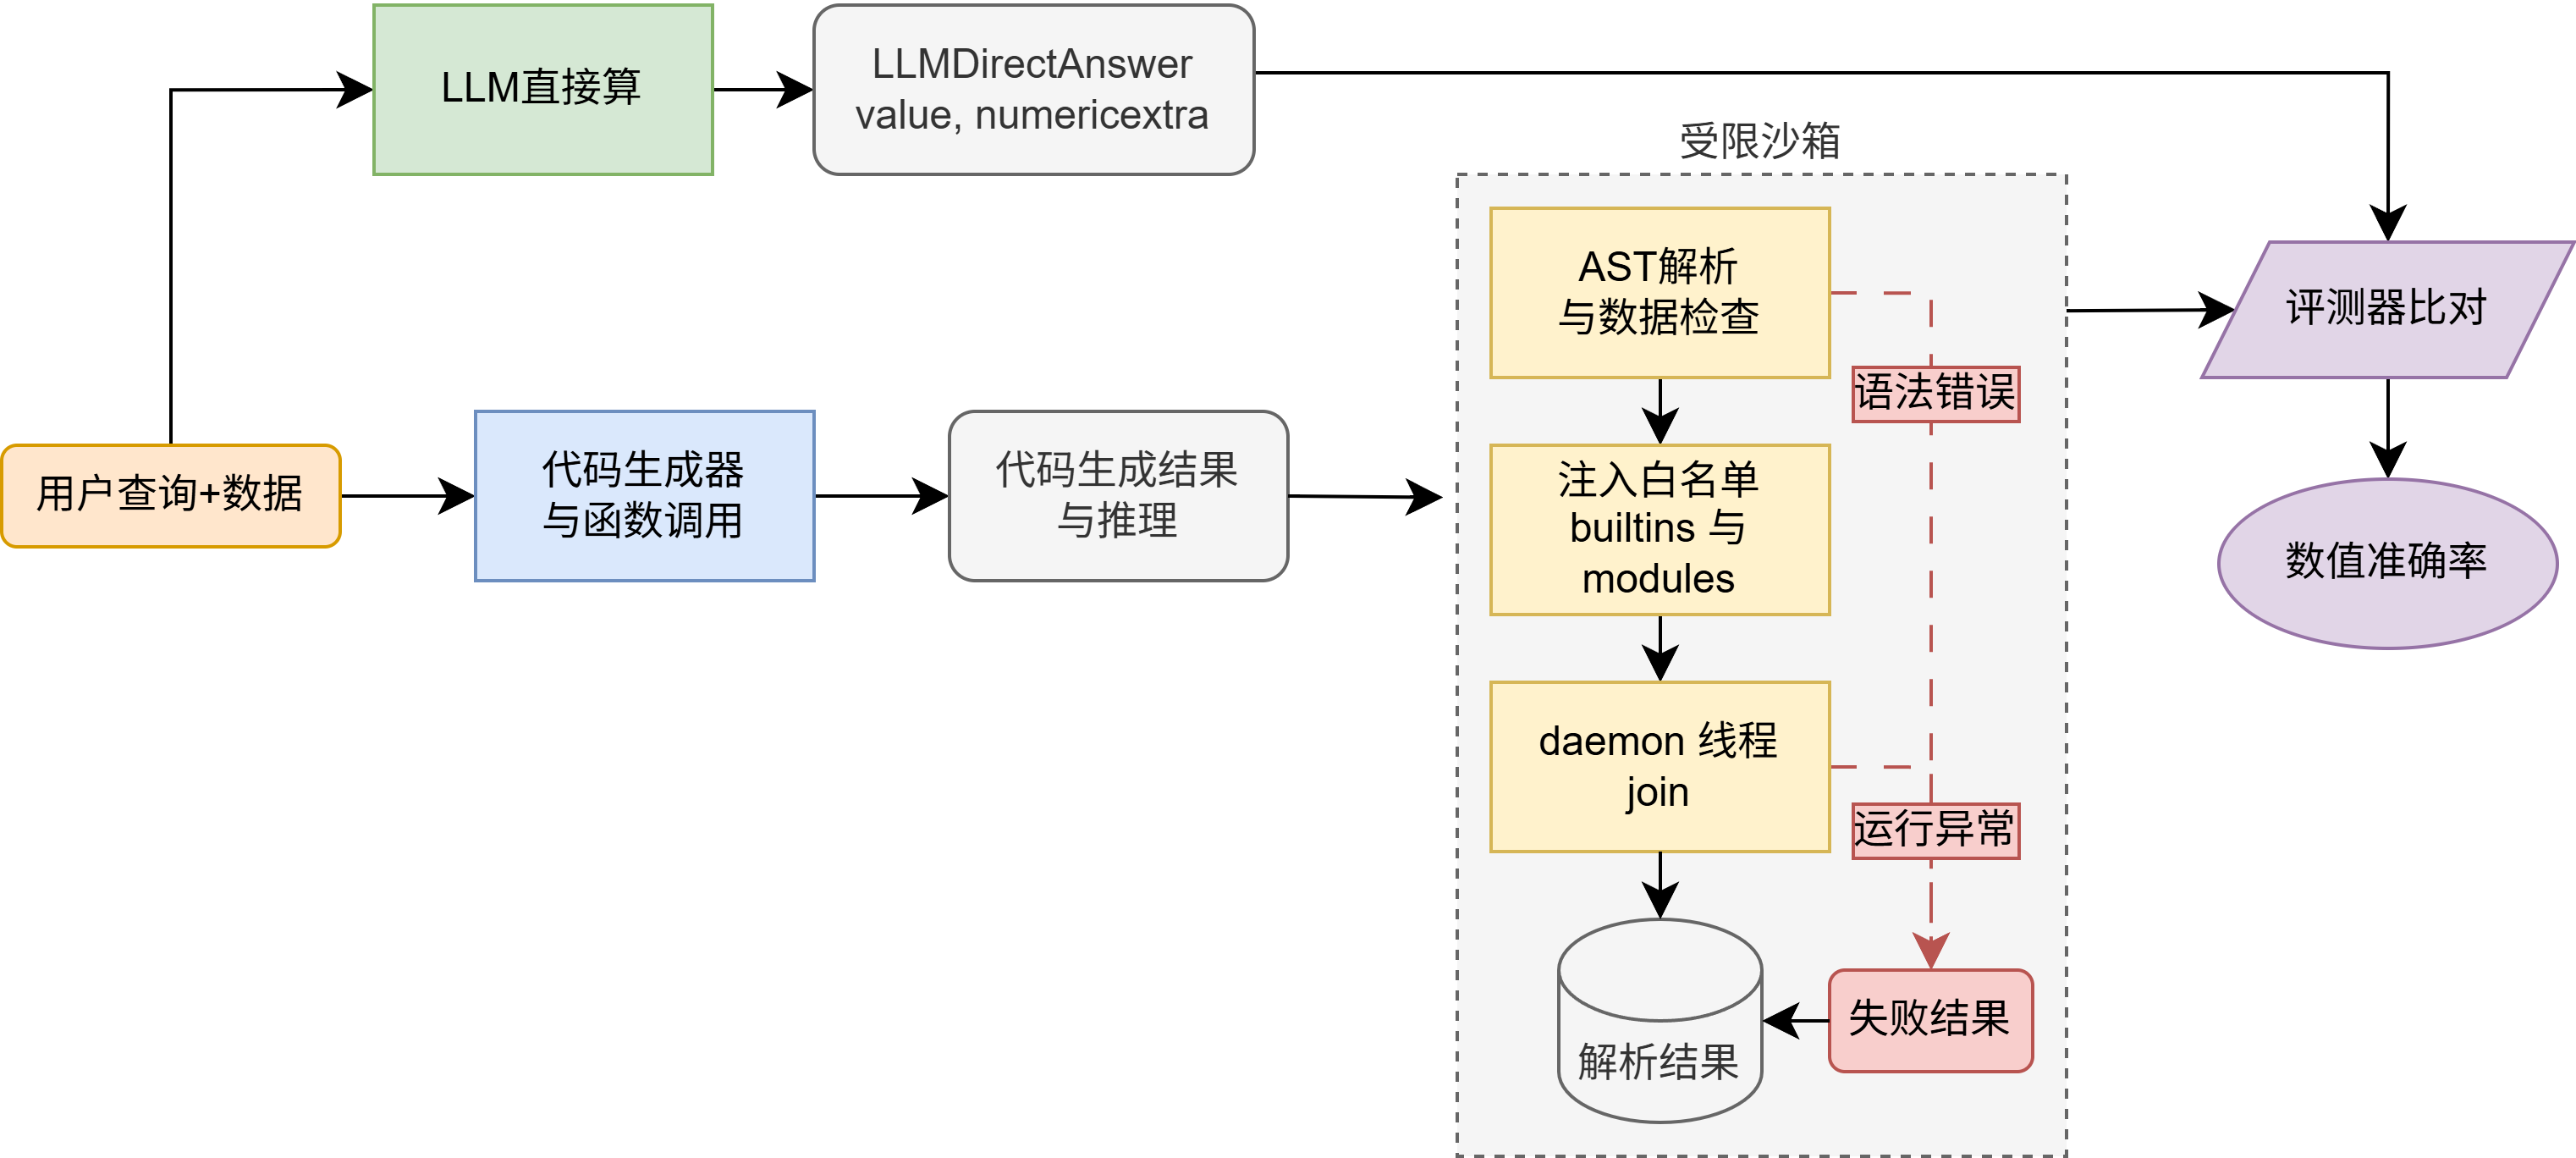
\includegraphics[width=0.78\linewidth,height=0.32\textheight,keepaspectratio]{figures/code-gen-flow}
    \caption{代码生成与受限沙箱执行流程图}
    \label{fig:code-gen-flow}
\end{figure}

第一是位于 \texttt{src/\bk{}analysis/\bk{}code\_\bk{}generator.\bk{}py} 的代码生成器，
通过 OpenAI 兼容协议下的 function calling 模式让大语言模型输出结构化
\texttt{CodeGenResult} 对象，包含 \texttt{code} 与 \texttt{reasoning}
两个字段。Prompt 中显式约定生成代码必须定义顶层函数 \texttt{compute(data)}，
\texttt{data} 由调用方注入，函数返回值即最终答案。第二是位于
\texttt{src/\bk{}tools/\bk{}code\_\bk{}executor.\bk{}py} 的受限沙箱，对生成代码做隔离执行。
第三是上层评测脚本，把代码生成器的输出送入沙箱执行并比对期望值。

受限沙箱的设计借鉴了 Schick 等 \cite{ref21} 在 Toolformer 中关于工具
调用安全边界的论述，但裁剪到本文场景下的最小可用形态，包含四项约束。
其一是显式 builtins 白名单。沙箱仅暴露 \texttt{abs}、\texttt{sum}、
\texttt{max}、\texttt{min}、\texttt{round}、\texttt{sorted}、
\texttt{enumerate}、\texttt{iter}、\texttt{next} 等数据处理类内置函数，
对 \texttt{open}、\texttt{eval}、\texttt{exec}、\texttt{compile}、
\texttt{\_\bk{}\_\bk{}import\_\bk{}\_\bk{}} 等高危内置实施显式黑名单。其二是模块白名单。
沙箱将 \texttt{math} 与 \texttt{statistics} 两个只读数学库注入受限
全局命名空间，禁止生成代码通过 \texttt{import} 引入任何其他模块。
其三是墙钟超时。每次调用 \texttt{compute(data)} 在 daemon 线程内执行，
通过 \texttt{Thread.\bk{}join(timeout)} 实现 5 秒墙钟超时，避免生成代码中
意外死循环阻塞主流程。其四是结构化错误捕获。语法错误、缺函数、运行时
异常与超时四类失败模式统一封装在 \texttt{ExecutionResult} 对象中返回，
不会以异常形式污染上游评测脚本。

需要明确的是，本文设计的沙箱属于轻量原型，主动放弃了完整的安全隔离。
真实生产环境下应当使用 RestrictedPython、Pyodide 或 Docker 容器实现
进程级隔离 \cite{ref23}。本文限定在毕业设计研究范围内，沙箱的核心
目标是为代码生成可靠性的可重复测量提供执行通道，而非抵御主动恶意攻击。
完整的安全沙箱方案在 \ref{sec:future-work} 节作为未来工作展开。

\subsubsection*{4.2.2 \quad 三档消融实验设计与核心结果}

为量化代码生成与执行带来的准确率提升，本文构建了 18 条覆盖六类统计模式
的评测集 \texttt{code\_\bk{}exec\_\bk{}bench.\bk{}jsonl}，详见
\reftab{tab:code-bench-design}。六类模式分别对应平均、极值、求和、差值、
计数、排序，每类用例都故意包含若干边界情形，例如平均值类中含 24.95 的
银行家舍入边界、计数类中含 35.0 的高温阈值平等、求和类中含条件求和。
每条用例标注期望值与容差，并按答案结构分为标量、日期、日期加数值复合、
时刻加数值复合、有序列表共五种期望类型。

\begin{table}[!ht]
    \centering
    \caption{代码执行评测集任务分布}
    \label{tab:code-bench-design}
    \song\wuhao
    \begin{tabular}{lrll}
        \toprule
        类别 & 用例数 & 期望答案类型 & 设计要点 \\
        \midrule
        平均 average & 5 & scalar & 含整除、近似与银行家舍入边界 24.95 \\
        极值 extreme & 3 & date / time + value & 同时返回日期或时刻与对应数值 \\
        求和 sum & 2 & scalar & 7 天累计与高温日条件求和 \\
        差值 diff & 4 & scalar 或 date + value & 日较差最大、跨日极差、同比差 \\
        计数 count & 2 & scalar & 含 35.0 °C 高温阈值平等 \\
        排序 sort & 2 & ordered\_list / date & Top-$K$ 排序与第二高温日期 \\
        \midrule
        \multicolumn{1}{c}{合计} & 18 & --- & --- \\
        \bottomrule
    \end{tabular}
\end{table}

实验设计三档消融以隔离不同来源的能力贡献。\texttt{oracle} 档直接读取
期望值，作为评测器自校验天花板，验证比较函数本身的正确性。
\texttt{llm\_\bk{}direct} 档让大语言模型同时看到 query 与 data，但 prompt
明确禁止生成代码，要求其直接给出数值答案，作为大语言模型自由发挥的
对照。\texttt{llm\_\bk{}with\_\bk{}code} 档让大语言模型生成 \texttt{compute(data)}
代码并送入受限沙箱执行，取沙箱返回值作为最终答案。三档使用同一被测
模型 GLM-5.1，避免引入模型差异。

核心结果见 \reftab{tab:code-eval-overall}。\texttt{oracle} 档准确率
100.0\%，证明评测器自身没有偏差。\texttt{llm\_\bk{}direct} 档数值准确率
仅为 66.7\%，\texttt{llm\_\bk{}with\_\bk{}code} 档数值准确率提升至 88.9\%，
两档之间存在 22.2 个百分点的差距。代码生成率与代码可执行率均为 94.4\%，
表明大语言模型在 function calling 模式下生成可执行代码的能力是稳定的，
失败主要来自单条用例上的算法错误而非工具调用失败。

\begin{table}[!ht]
    \centering
    \caption{代码执行三档消融总表}
    \label{tab:code-eval-overall}
    \song\wuhao
    \begin{tabular}{lccc}
        \toprule
        指标 & oracle & llm\_direct & llm\_with\_code \\
        \midrule
        数值准确率 & 100.0\% & 66.7\% & 88.9\% \\
        代码生成率 & --- & --- & 94.4\% \\
        代码可执行率 & --- & --- & 94.4\% \\
        \bottomrule
    \end{tabular}
\end{table}

按用例类别拆分后差距进一步放大，详见 \reftab{tab:code-eval-category}。
极值类用例上 \texttt{llm\_\bk{}direct} 准确率为 0.0\%，\texttt{llm\_\bk{}with\_\bk{}code}
为 66.7\%，差距 66.7 个百分点。计数类用例上 \texttt{llm\_\bk{}direct} 为
50.0\%，\texttt{llm\_\bk{}with\_\bk{}code} 为 100\%，差距 50 个百分点。求和与
排序两类则两档持平在 100\%。这一分布揭示了一条规律：大语言模型在简单
累加与天然排序任务上能够依靠语料能力做对，但只要任务需要持续跟踪
中间状态，例如在找最大值的同时记录对应日期，就会犯错。这一现象
与 \ref{sec:problem-modeling} 节归纳的数值漂移类幻觉吻合，根本
原因在于生成式模型缺乏可写的外部中间状态。代码执行的工程意义即
在于补上这一缺失——在沙箱里给模型一支笔与一张草稿纸，把心算
换成笔算 \cite{ref20}。

\begin{table}[!ht]
    \centering
    \caption{代码执行评测按用例类别拆分}
    \label{tab:code-eval-category}
    \song\wuhao
    \begin{tabular}{lrccc}
        \toprule
        类别 & 用例数 & llm\_direct & llm\_with\_code & 差距 \\
        \midrule
        极值 extreme & 3 & 0.0\% & 66.7\% & $+66.7$ pp \\
        计数 count & 2 & 50.0\% & 100.0\% & $+50.0$ pp \\
        平均 average & 5 & 80.0\% & 100.0\% & $+20.0$ pp \\
        求和 sum & 2 & 100.0\% & 100.0\% & 持平 \\
        排序 sort & 2 & 100.0\% & 100.0\% & 持平 \\
        差值 diff & 4 & 75.0\% & 75.0\% & 持平（命名漂移） \\
        \bottomrule
    \end{tabular}
\end{table}

\subsubsection*{4.2.3 \quad 大语言模型直算的四类典型幻觉模式}

通过对 \texttt{llm\_\bk{}direct} 档 6 条失败用例的逐条分析，本文归纳出大
语言模型在数值任务上的四类典型幻觉模式，每类都构成代码执行不可替代
的具体证据。

第一类是数数错误，对应用例 \texttt{count\_\bk{}001\_\bk{}rainy\_\bk{}days}。该用例
要求统计 14 天中降水量大于 0 的天数，正确答案为 7。大语言模型在
\texttt{reasoning} 字段中正确列举出了 7 个日期 04-02、04-03、04-05、
04-08、04-09、04-12、04-14，但 \texttt{value} 字段却给出了 6。这种
推理过程与最终答案自相矛盾的幻觉是最危险的形式，用户阅读 reasoning
通常会被说服，难以察觉数值错误。

第二类是舍入不一致，对应用例 \texttt{avg\_\bk{}005\_\bk{}feels\_\bk{}like}。8 小时
体感温度均值精确计算结果为 24.95，使用 Python \texttt{round} 的银行家
舍入向偶数舍入应得 24.9。大语言模型给出的答案是 25.0，并在 reasoning
中说明 24.95 保留 1 位小数为 25.0，反映其默认采用中学教科书的四舍五入
规则。这种语境敏感的精度幻觉在工程数据处理中是不可接受的，因为下游
所有数值处理都默认使用 Python 标准舍入。

第三类是 schema 不稳定，对应 \texttt{extreme\_\bk{}001} 至
\texttt{extreme\_\bk{}003} 与 \texttt{diff\_\bk{}001\_\bk{}max\_\bk{}diurnal} 共 4 条用例。
这些用例要求同时给出哪一天与对应数值，例如返回字典
\texttt{\{date: 2025-07-03, tempMax: 36.8\}}。Prompt 中已经明确要求
把日期放在 \texttt{value} 字段、把数值放在 \texttt{numeric\_\bk{}extra}
字段，但大语言模型在 function calling 下仍只填写日期字段，把数值留
作自由文本。Schema 的可靠性随复杂度上升急剧下降是大语言模型应用工程
中的经典痛点 \cite{ref22}。

第四类是字段命名漂移，仅出现在 \texttt{llm\_\bk{}with\_\bk{}code} 档的
\texttt{diff\_\bk{}001} 用例中。生成代码逻辑完全正确，找出了温差最大的
2025-09-18 一天，温差 22.7 摄氏度，但返回字典字段名为 \texttt{range}
而非期望的 \texttt{tempDiff}。这一失败模式与前三类性质不同，反映了
大语言模型在数据建模时命名约定不严格，可以通过更严格的 schema 约束
或下游适配层缓解。

将 4.1 与 4.2 两节合并观察，本文已经在分级 ID 编造、权威标准引用、
数值统计计算三个维度上量化了大语言模型自由发挥的不可靠性，并分别用
混合检索、确定性分级器、代码生成与受限沙箱执行三类机制构成了完整的
工具学习与计算辅助闭环。下一节将进一步讨论如何把这些机制的输出整合为
面向用户的自适应气象决策报告。

% ===== END: 草稿/4_2_代码生成 =====


% ===== BEGIN: 草稿/4_3_报告生成 =====
% =============================================================================
% 4.3 自适应气象决策报告生成技术
% 草稿版本：v0.4 (2026-05-07)
%   v0.1：完成正文初稿。
%   v0.3：按导师意见 9 规范化报告片段排版。
%   v0.4：按导师意见 10 把第 4 章整体小结从本节末段迁出到独立的
%        \subsection{本章小结}（4_4_本章小结.tex，label sec:chap4-summary），
%        本节末段仅保留承接句指向 4.4 节，避免与 4.4 节重复叙述。
%        ① 在文件顶部定义局部 reportsnippet 环境，提供"档位标签 +
%           分隔线 + 左缩进正文"的统一视觉容器，替代原裸 quote 块。
%        ② 替换两个对照样例为更有冲击力的真实端到端评测产出：
%           a) 暴雨判定 → 雾/驾车安全 (decision_006_fog)。full 档直接
%              给出 GB/T 27964-2011 雾的预报等级 4 档对照表（轻雾/雾/
%              浓雾/强浓雾），LLM-as-judge 专业性 5/5 vs ablated 3/5，
%              是 30 条端到端用例里专业性差距最大的对照之一；
%           b) 洗车 → 户外活动 (decision_001_outdoor)。full 档给出
%              GB/T 28592-2012 大雨档 25.0--49.9 毫米精确区间 +
%              雨势猛烈可读化解释，比洗车指数更能体现 RAG 在数值阈值
%              上的提取能力。
%        ③ 摘选片段忠实于 experiments/results/e2e_eval_20260505_183622.json
%           真实输出（可由该文件 raw_outputs[0].ablated/full 中按 id
%           检索复核），仅去除 markdown 表格与 emoji 等不属于决策文本
%           的视觉装饰，保留全部数值与 GB/T 编号。
% 字数：约 1750 字（不含 reportsnippet 块）
% 风格规则：v0.2 风格（无 \textbf / \textit / 引例括号 / 双引号 / 破折号）
% 引用：\cite{ref1, ref9, ref18, ref20}
% 图表：
%   - 表 \reftab{tab:report-template-routing}  四类场景与模板要素对应
%   - 表 \reftab{tab:report-judge-summary}     双档 LLM-as-judge 4 维度对照（节略，详见 5.2.2）
%   - reportsnippet 块 ×4：雾/驾车 与 户外活动 两个用例的 ablated vs full 对照
% 依赖宏包：booktabs / tabularx（主稿已加载）
% =============================================================================

% ----- 局部环境：reportsnippet -----
% 用法：
%   \begin{reportsnippet}{档位}{用例描述}
%       报告正文（可多段、可含 \texttt{...} 字段名）
%   \end{reportsnippet}
% 视觉效果：顶部"[档位] 用例描述"小标题（黑体），下接 0.4pt 横线，
%   正文整体左缩 1.2em、右缩 0.5em，正文字号与正文相同，便于读者一眼
%   分辨"这是被引模型输出"而非论文叙述。
\makeatletter
\newenvironment{reportsnippet}[2]{%
    \par\addvspace{0.5em}%
    \noindent
    {\hei\wuhao\fbox{\,#1\,}}\quad{\song\wuhao #2}\par
    \vspace{0.05em}%
    \noindent\rule{\linewidth}{0.4pt}\par
    \vspace{0.25em}%
    \begingroup
    \song\wuhao
    \leftskip=1.2em \rightskip=0.5em
    \parindent=0pt
}{%
    \par\endgroup
    \addvspace{0.5em}%
}
\makeatother

\subsection{自适应气象决策报告生成技术}
\label{sec:report-generation}

前述双通路 RAG 与代码生成加受限沙箱机制分别给出了带权威出处的语义
标签与可信的数值统计结果。然而面向终端用户的输出不是这些孤立的中间
产物，而是一份按场景组织的自然
语言决策报告。气象决策报告的具体形态高度依赖任务类型。日常查询场景下
用户只关心当前与未来若干小时的事实数据；出行决策场景下用户关心的是从
出发地到目的地不同时段的多点天气以及对应的穿衣与携物建议；户外作业与
预警场景下用户关心的是一份带权威分级与国标出处的安全结论。一份能够覆盖
这些异构场景的报告生成机制，必须解决信息整合、模板选择与引用规范三个
耦合问题。本节据此设计了基于 System Prompt 编排的自适应报告生成方案，
并以端到端用例对照说明其相对于无 RAG 基线的提升。

\subsubsection*{4.3.1 \quad 报告生成的设计需求与三类输入整合}

报告生成层位于 ReAct 循环的最后一步 \cite{ref18}，其输入由三类异构片段
构成。第一类是天气工具返回的事实数据，包含温度、风力、降水、湿度、能见度
等标量值与时序数组。第二类是 \texttt{bridge\_\bk{}weather\_\bk{}data} 与
\texttt{search\_\bk{}knowledge} 返回的语义解读，包含分级名、影响描述与国标
出处。第三类是 \texttt{compute(data)} 沙箱执行返回的统计结果，包含具体
数值与对应的代码推理过程。三类片段在数据形态、置信度来源与组织方式上
各不相同，简单拼接会产生信息冗余、出处遗漏或数值与等级冲突等问题。

报告生成的设计目标是把上述三类片段按统一结构编排为面向决策的自然语言
输出，同时保证三条不变性。第一是事实优先。数值数据必须先于解读出现，
避免大语言模型用主观叙述覆盖客观读数。第二是出处必引。凡涉及分级判定
或权威性结论的句子，引用源必须保留在报告中而不被改写或省略。第三是
场景对齐。回答内容应聚焦用户实际在场的时间地点，不输出与决策无关的
冗余信息。Kim 等 \cite{ref1} 在 ClimateAgent 中通过多智能体协作实现
类似的场景编排，本文受其启发但裁剪到单智能体形态，把场景编排逻辑下沉到
System Prompt 而非额外引入编排智能体。

\subsubsection*{4.3.2 \quad System Prompt 驱动的多场景报告模板}

本文不采用基于外部 DSL 的硬模板方案，而是把场景模板与编排规则编码到
\texttt{src/\bk{}config/\bk{}settings.\bk{}py} 中的 \texttt{SYSTEM\_\bk{}PROMPT} 字段。
该方案在工程实现上的优势是模板修改不需要改动核心代码，仅需调整 prompt
文本即可生效，便于在多场景任务中快速迭代路由规则与约束策略。这一设计与
LLM Agent 在配置化编排与可组合链路方面的工程实践一致 \cite{ref10,ref15,ref18}。
System Prompt 把报告生成约束分为四组规则。
工具使用规则定义了从用户问题到工具调用序列的路由路径。RAG 知识检索规则
定义了双通路 RAG 的强制调用条件与引用源不可省略约束。语义桥接调用约束
定义了数值到分级判定必须经过 \texttt{bridge\_\bk{}weather\_\bk{}data} 而不能由
大语言模型自行脑补阈值。出行场景推理规则定义了多地点多时段的对齐方式，
例如早八到晚六从武汉到成都的查询应分别查武汉上午与成都傍晚两个时段，
不查武汉晚上或成都早上。

这一类规则的具体覆盖见 \reftab{tab:report-template-routing}，四类典型
气象决策场景在报告要素上的差异通过 System Prompt 显式编码，而非依赖大
语言模型的隐式偏好。

\begin{table}[!ht]
    \centering
    \caption{四类气象决策场景下报告要素的差异化编排}
    \label{tab:report-template-routing}
    \song\fontsize{9pt}{12pt}\selectfont
    \renewcommand{\arraystretch}{0.95}
    \begin{tabular}{llll}
        \toprule
        场景 & 主要工具调用 & 必出报告要素 & 引用强制 \\
        \midrule
        日常查询 & current\_weather + indices & 数值 + 体感解读 & 可选 \\
        出行决策 & forcast\_weather + indices + bridge & 多时段数值 + 穿衣建议 & 涉及阈值时强制 \\
        户外作业 & current\_weather + bridge + knowledge & 数值 + 分级 + 安全结论 & 强制 \\
        极端预警 & weather\_warning + bridge + knowledge & 预警等级 + 国标依据 + 应对建议 & 强制 \\
        \bottomrule
    \end{tabular}
\end{table}

\subsubsection*{4.3.3 \quad 三类输入的编排逻辑与典型报告对照}

报告编排的具体次序遵循事实先行原则。先以表格或要点形式列出 API 工具
返回的数值数据，再附加 \texttt{bridge\_\bk{}weather\_\bk{}data} 返回的等级与
国标出处，最后给出基于这两类信息的决策建议。一旦涉及统计计算需求，
\texttt{compute(data)} 的执行结果会以具体数值加计算依据的方式嵌入到
事实数据段，避免大语言模型在数值聚合上的幻觉。Hong 等 \cite{ref20} 关于
让大语言模型直算等价于无草稿心算的论述在报告生成阶段同样适用，因为
最终输出本身就是一种聚合性表达，只要中间环节出现一次数值幻觉就会污染
整段报告。

下面以两个典型用例对比 \texttt{full} 档（含双通路 RAG）与 \texttt{ablated}
档（仅 9 个天气工具）的报告输出差异。两档共享同一份意图识别前置与同一份
天气数据，差异仅来自报告生成阶段是否能够调用 \texttt{search\_\bk{}knowledge}
与 \texttt{bridge\_\bk{}weather\_\bk{}data}。两个对照用例的报告片段均摘选自
\texttt{e2e\_\bk{}bench.\bk{}jsonl} 端到端评测的真实输出，仅删除了 markdown
表格与图标等不属于决策文本的视觉装饰，保留全部数值与 GB/T 编号原文。

第一个对照用例 \texttt{decision\_\bk{}006\_\bk{}fog} 是用户查询明天南京的雾
有多大、开车安全吗。两档都正确判断了明天南京无明显雾情，但对雾天驾驶
安全的论证方式截然不同，两档完整报告片段见 \refcase{case:fog-cmp}。

\begin{casebox}
    \caption{\texttt{decision\_\bk{}006\_\bk{}fog} 用例 \texttt{ablated} 档与 \texttt{full} 档报告片段对照}
    \label{case:fog-cmp}
    \begin{reportsnippet}{ablated}{decision\_\bk{}006\_\bk{}fog · LLM-as-judge 专业性 3.0 / 5.0}
    明天南京没有雾。凌晨湿度最高约 76\%，属于偏高但远未达到起雾条件，通常
    需大于等于 90\% 以上且温差大才易形成辐射雾。

    总体判断：明天开车是安全的。无雾、无雨，能见度正常；无天气预警生效；
    风力不大，上午东南风 1 至 3 级，下午南风 3 至 4 级。
    \end{reportsnippet}

    \begin{reportsnippet}{full}{decision\_\bk{}006\_\bk{}fog · LLM-as-judge 专业性 5.0 / 5.0}
    明天南京无明显雾情。全天无降水，凌晨湿度虽偏高（最高 76\%），但天气
    状况为晴，不具备成雾条件；当前无大雾预警信息。

    依据 GB/T 27964-2011《雾的预报等级》（中国气象局）：
    轻雾对应能见度 1 至 10 km，影响较小，开示廓灯或近光灯并降速即可；
    雾对应能见度 500 至 1000 m，需开近光灯加前后雾灯，保持车距；
    浓雾对应能见度 50 至 500 m，触发大雾黄色预警，道路与机场显著受影响；
    强浓雾对应能见度小于 50 m，触发红色预警，严重威胁交通安全。

    明天南京预报为晴到阴，能见度远高于轻雾阈值（1 km），不存在雾天驾驶
    风险。
    \end{reportsnippet}
\end{casebox}

\texttt{ablated} 档给出的"通常需大于等于 90\% 才易形成辐射雾"是合理的
气象常识，但既无标准号支撑，也无能见度对照表帮助用户判断不同雾况下的
具体驾驶动作。\texttt{full} 档直接给出 GB/T 27964-2011《雾的预报等级》
4 档全表，把抽象的雾况判断转化为可对照的能见度区间与具体驾驶建议，
构成了完整可溯源的专业表达。LLM-as-judge 在专业性维度上对该条 ablated
档给 3.0 分而对 full 档给 5.0 分，2.0 分的差距正是双通路 RAG 在权威
分级表上的不可替代价值的直接量化。

第二个对照用例 \texttt{decision\_\bk{}001\_\bk{}outdoor} 是用户查询明天武汉
适合户外活动吗。两档都识别到明天夜间有大雨这一关键事实，但对大雨这一
分级的支撑力度差异显著，两档完整报告片段见 \refcase{case:outdoor-cmp}。

\begin{casebox}
    \caption{\texttt{decision\_\bk{}001\_\bk{}outdoor} 用例 \texttt{ablated} 档与 \texttt{full} 档报告片段对照}
    \label{case:outdoor-cmp}
    \begin{reportsnippet}{ablated}{decision\_\bk{}001\_\bk{}outdoor · 关键事实 5/5、专业性 4/5}
    明天武汉白天适合户外活动，建议安排在上午或下午 4 点以后，避开正午高温；
    傍晚起需关注降雨，夜间大雨不宜外出。

    注意事项：高温防暑（最高温达 32 °C，湿度高达 91\%，体感闷热）；夜间
    大雨，不建议安排傍晚及夜间的户外活动，如需外出请携带雨具。
    \end{reportsnippet}

    \begin{reportsnippet}{full}{decision\_\bk{}001\_\bk{}outdoor · 关键事实 5/5、专业性 5/5}
    明天武汉白天适合户外活动，但傍晚到夜间不适合。

    夜间不适宜：傍晚后有大雨，根据《降水量等级》（GB/T 28592-2012），
    大雨指 24 小时降水量 25.0 至 49.9 毫米，雨势猛烈，能见度明显下降，
    地面易积水，不适合户外活动。

    最佳时段为上午 6 至 12 点（晴到多云、温度适宜），次佳时段为下午
    12 至 16 点（阴天但无雨，注意防晒），避免时段为傍晚 18 点后（有大雨，
    建议室内活动）。
    \end{reportsnippet}
\end{casebox}

\texttt{ablated} 档把大雨当作不证自明的常识词使用，回答语气自信但缺少
分级阈值依据。\texttt{full} 档则直接调用通路 B 给出 GB/T 28592-2012
中大雨档的精确区间 25.0 至 49.9 毫米与雨势猛烈、能见度明显下降、地面
易积水三类后果描述，把日常用语大雨转化为可量化、可决策的工程化表达。
LLM-as-judge 在专业性维度对 full 档给出满分 5.0；在 30 条端到端用例的
\texttt{decision\_\bk{}support} 类 6 条对照中，\texttt{ablated} 档通过率
仅 50\%，\texttt{full} 档为 100\%，差距 50 个百分点的端到端表现差距
即源自这一类报告生成阶段的引用纪律差异。

\subsubsection*{4.3.4 \quad 报告质量的端到端验证概要}

为量化上述报告生成机制的实际价值，本文采用 LLM-as-judge 4 维度评分
作为报告质量的代理指标，每条用例由独立大语言模型按事实性、完整性、
专业性、流畅性四个 0 至 5 区间维度打分。在 30 条覆盖六类场景的端到端
评测集上，两档对照结果的核心数据见 \reftab{tab:report-judge-summary}。

\begin{table}[!ht]
    \centering
    \caption{两档报告质量 LLM-as-judge 评分摘要}
    \label{tab:report-judge-summary}
    \song\wuhao
    \begin{tabular}{lccc}
        \toprule
        维度 & ablated & full & 差距 \\
        \midrule
        事实性 & 4.07 & 3.90 & $-0.17$ \\
        完整性 & 4.93 & 4.87 & $-0.06$ \\
        专业性 & 3.10 & 3.47 & $+0.37$ \\
        流畅性 & 4.97 & 5.00 & $+0.03$ \\
        综合 & 4.27 & 4.31 & $+0.04$ \\
        \bottomrule
    \end{tabular}
\end{table}

四个维度的差距分布揭示了报告生成阶段一个值得关注的现象。事实性、
完整性、流畅性三档接近持平甚至 \texttt{ablated} 档略胜，差距全部集中
在专业性维度的 $+0.37$ 个分差。这一结果可以从两个角度解读。第一，
大语言模型本身在表达流畅性与结构完整性上有较强的语料先验，无 RAG 时
也能写出看起来合理的报告。第二，当评估聚焦在分级、引用、阈值依据这
一专业维度时，双通路 RAG 的价值才真正显现出来。仅看综合分会得到 RAG
价值有限的错误印象，而拆分到专业性这一更细的维度才能反映真实差距。
完整的端到端评测设计、断言定义与按场景类别拆分的详细数据见
\ref{sec:e2e-eval} 节。

值得注意的是 \texttt{full} 档自身在专业性维度上的得分 3.47 仍未达到
满分。逐条分析失败用例可发现，4 条 \texttt{full} 档未通过的用例共同特征
是大语言模型在 RAG 结果中确实拿到了相关分级阈值，但在最终报告生成时
省略了 GB/T 编号。这一现象在 \ref{sec:semantic-bridge} 节描述为通路 B
单测层面的引用真实性已达到 100\% 但端到端集成后衰减到 26.7\%。这种从
模块层到集成层的指标衰减是单模块评测无法捕捉的盲区，构成
\ref{sec:future-work} 节关于
显式引用强制注入与生成后校验的具体改进方向。

% --- 4.3 节末段过渡（4 章整体小结迁出至独立 \subsection 4.4）---
报告生成阶段的设计与实证至此告一段落。从 \ref{sec:semantic-bridge} 节
双通路 RAG 算法到本节自适应报告模板，三组核心组件在数据流向上依次完成
数值到语义、数值到统计结果、多源信息到自然语言报告的串接，已具备进入
本章小结收口的条件，详见 \ref{sec:chap4-summary} 节。

% ===== END: 草稿/4_3_报告生成 =====


% ===== BEGIN: 草稿/4_4_本章小结 =====
% =============================================================================
% 4.4 本章小结
% 草稿版本：v0.1 (2026-05-07)
% 起草动机：按导师意见 10，第 4 章必须包含独立的"本章小结"小节，承担
%           4.1 双通路 RAG / 4.2 代码生成与受限沙箱 / 4.3 自适应报告
%           生成三组件的统一收口，并把模块层与集成层的核心数据汇成
%           一段集中证据，引出第 5 章实验验证。原 4_3_报告生成.tex
%           末段的章节过渡块迁出到本文件并扩写为独立小节。
% 字数：约 750 字
% 风格规则：v0.2 风格（无 \textbf / \textit / 引例括号 / 双引号 / 破折号）
% 引用：暂无新增引用（核心数据来自 4.1 / 4.2 / 4.3 节及第 5 章评测）
% 图表：无新增（核心数据已在前 3 节图表中给出，本节仅以叙述方式收口）
% 依赖宏包：booktabs / tabularx（主稿已加载）
% =============================================================================

\subsection{本章小结}
\label{sec:chap4-summary}

本章针对开题报告中提出的异构数据语义化与数值理解幻觉两个研究问题，
构建了由双通路 RAG、代码生成与受限沙箱、自适应报告生成三个组件协同
的完整气象数据统计分析方法。\ref{sec:semantic-bridge} 节解决了从数值
到带引用源的语义标签这一离散映射任务，\ref{sec:code-execution} 节
解决了从原始数据到统计结果这一连续计算任务，\ref{sec:report-generation}
节解决了把事实数据、语义解读、统计结果三类异质输入编排为场景化决策
报告这一信息整合任务。三组件在数据流向上首尾相接，分别对应大语言
模型在精确归属、精确计算、专业表达三类能力上的内在边界，并以确定性
组件外置的工程范式将这些边界转化为可量化、可控的工程问题。

\ref{sec:semantic-bridge} 节通过双通路 RAG 架构把概念检索与数值
归属分离。通路 A 在 60 条混合检索评测集上以 $\alpha = 0.9$ 取得
Top-1 命中率 85.0\% 与 MRR 0.908，并量化了最优权重随知识库体量
漂移的工程结论；通路 B 在 71 条覆盖 9 类要素的语义桥接评测集上把
\texttt{grade\_\bk{}id} 准确率与 \texttt{citation} 真实性同时提升到
100\%，相对让大语言模型直接处理裸数据的 \texttt{llm\_\bk{}baseline}
基线在 \texttt{grade\_\bk{}id} 严格命中率上形成 94.4 个百分点的差距。
桥接前后模型上下文对比（\reffig{fig:bridge-context-compare}）从可视
角度直接呈现了这一组件的工程价值。

\ref{sec:code-execution} 节通过结构化数据契约约束的代码生成与白名单
受限沙箱，把统计计算从大语言模型的自由发挥改造为确定性 Python 函数
执行。在 18 条覆盖最大值、平均值、阈值次数等 6 类计算任务的评测中，
\texttt{llm\_\bk{}with\_\bk{}code} 档数值准确率达到 88.9\%，比让大语言
模型直接给出数值答案的 \texttt{llm\_\bk{}direct} 档高出 22.2 个百分点。
失败用例集中暴露了大语言模型在伴随状态维护与离散计数任务上的
内在边界，这一边界与 \ref{sec:semantic-bridge} 节关于数值阈值排序
的边界共同构成本文确定性组件外置范式的两个量化锚点。

\ref{sec:report-generation} 节通过场景驱动的 System Prompt 与三条
不变性约束（事实优先、出处必引、场景对齐），把多源信息整合为可读、
可溯、可决策的自然语言报告。在 30 条覆盖 6 类场景的端到端评测中，
\texttt{full} 档相对去 RAG 的 \texttt{ablated} 档把任务通过率从
73.3\% 提升到 86.7\%，把权威标准引用率从 0\% 提升到 26.7\%，把
\texttt{decision\_\bk{}support} 类用例通过率从 50\% 提升到 100\%。
四维度 LLM-as-judge 评分进一步显示，事实性、完整性、流畅性三档接近
持平，差距全部集中在专业性维度的 $+0.37$ 分差，印证了双通路 RAG
的价值在专业表达层面的精准定位。

三组件的实证数据共同支撑本章方法论的有效性。下一章将在统一实验环境
下完成 5 套独立评测集共 214 条用例的系统化验证，按模块层与集成层
两个粒度系统报告全部评测设计、量化数据与失败模式分析。
% ===== END: 草稿/4_4_本章小结 =====



\sectionbreak

% ============================================================ %
% 第 5 章：实验验证（按导师意见 3 重构）
%   - 原 5.2.1--5.2.5 子小节提级为 5.2--5.6 \subsection
%   - 原章名"实验验证与总结"改为"实验验证"
%   - 新增 5.7 本章小结
%   - 原 5.3 全文总结 / 5.4 研究前景迁出到下方独立的第 6 章
% ============================================================ %
\section{实验验证}
\label{chap:evaluation}

% ===== BEGIN: 草稿/5_1_实验环境 =====
% =============================================================================
% 5.1 实验环境与数据集构建
% 草稿版本：v0.1 (2026-05-05)
% 字数：约 1500 字
% 风格规则：v0.2 风格（无 \textbf / \textit / 引例括号 / 双引号 / 破折号）
% 引用：\cite{ref14, ref15}
% 图表：
%   - 表 \reftab{tab:exp-env}            软硬件与依赖版本
%   - 表 \reftab{tab:dataset-overview}   5 份评测集统一汇总
% 依赖宏包：booktabs / tabularx（主稿已加载）
% =============================================================================

\subsection{实验环境与数据集构建}
\label{sec:exp-env}

为支撑 \ref{chap:semantic-bridge} 章方法论的完整实证，本章在统一的实验
环境下构建了 5 份独立评测集，形成由 4 个模块层评测加 1 个集成层评测组成
的实证体系。本节先说明软硬件与依赖版本，再交代 5 份评测集的统一构建原则
与可重现性工程要点。

\subsubsection*{5.1.1 \quad 软硬件环境与依赖版本}

实验在单机 Windows 10 工作站上运行，Python 运行时基于 Anaconda 环境管理。
被测大语言模型为智谱 GLM-5.1，通过 SiliconFlow 平台提供的 OpenAI 兼容
HTTP API 调用，温度全部置 0 以最大化结果可重复性。开源 LLM 体系的成熟
为本课题提供了可替换的实验底座 \cite{ref14}，本文核心方法论与具体被测
模型解耦，未来切换为本地部署模型不需要修改评测脚本。Agent 框架基于
LangChain 生态 \cite{ref15} 中的 \texttt{create\_agent} 与
LangGraph 的 \texttt{InMemorySaver}，分别承担 ReAct 循环编排与多轮对话
状态保持。完整环境清单见 \reftab{tab:exp-env}。

\begin{table}[H]
    \centering
    \caption{实验环境与关键依赖版本}
    \label{tab:exp-env}
    \song\fontsize{9pt}{12pt}\selectfont
    \renewcommand{\arraystretch}{0.95}
    \begin{tabular}{ll}
        \toprule
        类别 & 名称与版本 \\
        \midrule
        操作系统 & Windows 10 \\
        Python 运行时 & Python 3.11 (Anaconda 环境管理) \\
        LLM 主模型 & GLM-5.1 (SiliconFlow OpenAI 兼容协议，温度 0) \\
        嵌入模型 & BAAI/bge-m3 (1024 维，SiliconFlow) \\
        Agent 框架 & langchain 0.3 + langgraph 0.2 \\
        向量数据库 & ChromaDB (持久化模式) \\
        词法检索 & rank\_bm25 (倒排索引) \\
        数据校验 & Pydantic v2 (结构化输出) \\
        天气数据源 & 和风天气 API + Open-Meteo API \\
        \bottomrule
    \end{tabular}
\end{table}

\subsubsection*{5.1.2 \quad 评测集构建的统一原则}

本文 5 份评测集分别针对意图识别、通路 A 检索、通路 B 桥接、代码执行
与端到端任务完成率，覆盖从用户输入入口到最终决策报告的全链条。各评测集
的统一汇总见 \reftab{tab:dataset-overview}。

\begin{table}[H]
    \centering
    \caption{5 份评测集汇总}
    \label{tab:dataset-overview}
    \song\fontsize{9pt}{12pt}\selectfont
    \renewcommand{\arraystretch}{0.95}
    \begin{tabular}{llrl}
        \toprule
        评测集 & 评测对象 & 用例数 & 分类维度 \\
        \midrule
        \texttt{intent\_bench.jsonl} & 意图识别 + 参数补全 & 35 & 10 类场景 \\
        \texttt{rag\_retrieval\_bench.jsonl} & 通路 A 混合检索 & 60 & 8 类查询 \\
        \texttt{semantic\_bridge\_bench.jsonl} & 通路 B 语义桥接 & 71 & 9 类气象要素 \\
        \texttt{code\_exec\_bench.jsonl} & 代码生成 + 沙箱执行 & 18 & 6 类统计模式 \\
        \texttt{e2e\_bench.jsonl} & 端到端任务完成率 & 30 & 6 类真实场景 \\
        \midrule
        \multicolumn{2}{c}{合计} & 214 & --- \\
        \bottomrule
    \end{tabular}
\end{table}

5 份评测集的设计遵守三条统一原则。第一条是真实数据为底，结构化断言
为锚。所有用例均基于真实国家标准、真实和风天气与 Open-Meteo API 返回值
构造，未使用人工合成的伪数据。但评测断言不直接断言具体数值，而是断言
结构性证据，例如必须含温度数值、必须给具体日期、必须出现 GB/T 编号
等。这一设计保证了即便 API 返回值随时间漂移，评测断言依然可重复。
第二条是模块边界清晰，评测互不重叠。每份评测集只针对一个模块的能力
边界，例如通路 A 评测只评检索质量而不评意图识别，意图识别评测只评结构化
输出而不评 RAG 召回。这种切分使得失败定位可以精确到模块。第三条是
按用例类别细粒度切分。每份评测集都至少有 6 类以上的子类别，便于按子类
拆分发现差异化失败模式，例如通路 A 评测拆分到 8 类查询，端到端评测
拆分到 6 类场景。

知识库本身的可信性是上述检索类与桥接类评测的基础前提。本文采用分阶段
人工核对加权威资料库检索双重核验的方式，对 \texttt{data/knowledge/} 下三类
共 62 条知识条目所引用的 17 项国家标准、行业标准与国际规范逐一校验，
累计修正了 24 处问题。问题类型包括 1 处标准编号张冠李戴
GB/T 20484 误引为寒潮等级、3 处条款号错位 JGJ 80-2016 §3.0.4 应为
§3.0.8、4 处雾分级阈值与预警阈值混用、7 处 GB 50736-2012 I 级与 II 级
热舒适推荐值混用，以及 4 处业内惯例被错标为 official 标准等。一个值得
注意的现象是，知识库从首轮 38 条扩展到 62 条之后，错误率不降反升，从
首轮 13/38 即 34.2\% 上升到二轮新增 11/19 即 57.9\%，全库累计 24/62 即
38.7\%。这反映了知识库扩展过程中人工核对环节的不可省略性，复用同样的
标准引用模式并不能保证不出错。

\subsubsection*{5.1.3 \quad 评测框架的工程稳定性要点}

5 份评测集对应 5 套独立评测脚本，统一采用三层缓存加增量落盘加断点续跑
的工程实现。第一层缓存针对意图识别前置，按用户查询哈希索引；第二层
缓存针对 Agent 完整输出，按查询与模式名联合索引，端到端评测中两档
共享同一份意图识别结果以节省一半 LLM 调用；第三层缓存针对 LLM-as-judge
打分，按问答对哈希索引。所有缓存键计算包含 prompt 字面值的版本号
指纹，prompt 修改自动失效相关缓存。

每套评测脚本的 LLM 调用统一带 60 秒至 90 秒超时与 2 次重试，单次请求
最多约 3 分钟必定返回。主循环包裹在 \texttt{try/finally} 中，每条用例
完成后立即增量落盘三层缓存。任何时刻按下 \texttt{KeyboardInterrupt}
都不会丢失已完成进度，断点续跑直接从未完成用例开始。这一组工程加固
源自前期评测中遇到的 SiliconFlow 平台 socket idle hang 教训，是
评测可重现性的工程前提，与后续几节定量结果的可信度密切相关。

为支持研究的可复现性，本课题完整源代码、3 类共 62 条知识库、5 套
评测集 \texttt{jsonl} 文件、原始评测结果与一键运行脚本均已通过
公开 GitHub 仓库托管，仓库地址与简要目录结构详见附录。

% ===== END: 草稿/5_1_实验环境 =====


% ===== BEGIN: 草稿/5_2_意图评测 =====
% =============================================================================
% 5.2 意图识别与参数补全评测
% 草稿版本：v0.2 (2026-05-07)
%   v0.1：作为 5.2.1 子小节起草，依附于 5.2 节（典型气象任务场景下的技术验证）。
%   v0.2：按导师意见 3 与意见 5 重构。原 5.2.1 提级为 5.2 \subsection，
%        删除原 5.2 节级导言段（与 5.1 节 5 份评测集汇总表内容重叠）。
% 字数：约 1300 字
% 风格规则：v0.2 风格（无 \textbf / \textit / 引例括号 / 双引号 / 破折号）
% 引用：\cite{ref10, ref18, ref29}
% 图表：
%   - 表 \reftab{tab:intent-overall}     35 条总表
%   - 表 \reftab{tab:intent-by-category} 按场景拆分
% 依赖宏包：booktabs / tabularx（主稿已加载）
% =============================================================================

\subsection{意图识别与参数补全评测}
\label{sec:intent-eval}

意图识别与参数补全位于 ReAct Agent 链条的最前端，承担把自然语言查询
转化为结构化 \texttt{WeatherIntent} 对象的责任 \cite{ref18}。本节在
\texttt{intent\_\bk{}bench.\bk{}jsonl} 共 35 条用例上评测两个模块的联合表现，
评测脚本为 \texttt{experiments/\bk{}eval/\bk{}run\_\bk{}intent\_\bk{}eval.\bk{}py}。

评测集覆盖 10 类场景，包含 8 类单轮场景共 28 条、多轮上下文继承类
\texttt{context\_\bk{}inference} 共 3 条与对抗鲁棒类 \texttt{adversarial}
共 2 条。8 类单轮场景包括当前天气、逐小时预报、逐日预报、预警、生活
指数、历史日报、历史小时报与出行建议，其中出行建议类共 5 条专门压测
出发地、经停地与到达地三类地点角色的标注能力。多轮场景每条用例自带
\texttt{context} 字段，用于把上一轮对话摘要拼接到 prompt 中以构成
最简形式的对话状态测试。对抗鲁棒类用例包括与气象无关的电影查询，
用于验证 \texttt{recognizer} 不被诱导触发误识别。

评测指标分为两阶段共 9 项加 1 项端到端综合。\texttt{recognizer} 阶段
有 5 项指标，分别对应意图准确率、地点集合召回率与精确率、地点角色
准确率与时间字段识别率。\texttt{completer} 阶段有 3 项指标，对应
\texttt{is\_\bk{}complete} 判定准确率、\texttt{follow\_\bk{}up} 触发准确率
与 \texttt{notes} 字段覆盖率。综合指标 \texttt{end\_\bk{}to\_\bk{}end\_\bk{}pass\_\bk{}rate}
要求 9 项全部通过才算端到端通过，是论文核心指标。35 条用例的总体
结果见 \reftab{tab:intent-overall}。

\begin{table}[H]
    \centering
    \caption{意图识别与参数补全评测 9 项指标总表}
    \label{tab:intent-overall}
    \song\wuhao
    \begin{tabular}{lr}
        \toprule
        指标 & 数值 \\
        \midrule
        端到端通过率 & 91.4\% \\
        意图准确率 & 97.1\% \\
        地点角色准确率 & 100.0\% \\
        地点集合召回率 & 96.6\% \\
        地点集合精确率 & 95.6\% \\
        时间字段识别率 & 91.7\% \\
        \texttt{is\_\bk{}complete} 判定准确率 & 100.0\% \\
        \texttt{follow\_\bk{}up} 触发准确率 & 100.0\% \\
        \texttt{notes} 字段覆盖率 & 50.0\% \\
        \bottomrule
    \end{tabular}
\end{table}

总表层面 91.4\% 的端到端通过率虽已达到工程可用水平，但单一聚合指标
容易掩盖不同场景类别下能力边界的差异化表现。本文按用户实际查询场景
将评测集进一步划分为 10 个类别独立统计，覆盖单轮直问与多轮上下文
继承两个使用维度，按类别拆分后的端到端通过率分布详见
\reftab{tab:intent-by-category}。这一分布是后续讨论中识别系统真实
能力边界的关键证据，同时也为生产环境中按场景维度做分级可观测性
提供了直接的指标基线。

8 类单轮场景共 28 条用例端到端全部通过，对抗鲁棒类 2 条全部正确
触发 \texttt{unknown} 加友好追问，出行建议类 5 条全部通过，
departure、arrival 与 waypoint 三类地点角色识别准确率均达 100\%。
唯一的 \texttt{life\_\bk{}index} 失败来自单点 \texttt{recognizer} 抖动，但
\texttt{completer} 模块触发了正确追问，业务层面用户体验仍然正确。
真正能拉开差距的是多轮上下文继承类 \texttt{context\_\bk{}inference}，
该类 3 条用例端到端通过率仅为 33.3\%，是全部 10 个类别中最低的一项，
也是本节后续失败模式分析的核心。

\begin{table}[!t]
    \centering
    \caption{意图识别评测按场景类别拆分}
    \label{tab:intent-by-category}
    \song\fontsize{9pt}{12pt}\selectfont
    \renewcommand{\arraystretch}{0.95}
    \begin{tabular}{lrr}
        \toprule
        类别 & 用例数 & 端到端通过率 \\
        \midrule
        \texttt{adversarial} & 2 & 100.0\% \\
        \texttt{current\_\bk{}weather} & 4 & 100.0\% \\
        \texttt{daily\_\bk{}forecast} & 5 & 100.0\% \\
        \texttt{historical\_\bk{}daily} & 2 & 100.0\% \\
        \texttt{historical\_\bk{}hourly} & 2 & 100.0\% \\
        \texttt{hourly\_\bk{}forecast} & 5 & 100.0\% \\
        \texttt{life\_\bk{}index} & 4 & 75.0\% \\
        \texttt{travel\_\bk{}advice} & 5 & 100.0\% \\
        \texttt{weather\_\bk{}warning} & 3 & 100.0\% \\
        \texttt{context\_\bk{}inference} & 3 & 33.3\% \\
        \bottomrule
    \end{tabular}
\end{table}

回到 \texttt{context\_\bk{}inference} 类的 33.3\% 通过率，与单轮场景
之间 66.7 个百分点的差距清晰暴露了系统在多轮长程依赖上的真实瓶颈。
失败用例的共同特征是，当用户
查询仅切换其中一个槽位时，例如从查北京明天天气切换为问那成都呢，
大语言模型能够正确识别地点切换，但会遗漏从上下文继承的时间字段
\texttt{date} 等于明天。当查询同时切换意图与隐式继承多个槽位时，
例如上一轮问武汉明天天气，本轮问那需要防晒吗，意图切换正确但
\texttt{locations} 与 \texttt{time} 两个槽位都被重置为空。这一现象
表明大语言模型在单轮意图理解上已接近人类水平，但结构化字段的跨轮
继承能力是另一个独立的能力维度。单纯把上下文摘要拼接到 prompt 中
不足以稳定实现地点继承加时间继承加意图切换的复合任务，必须借助显式
对话状态跟踪机制 \cite{ref29}。这一局限性在 \ref{sec:future-work} 节
作为未来工作展开。

分层架构的容错价值同样需要在失败用例分析中专门指出。在 \texttt{life\_\bk{}index}
类用例 \texttt{index\_\bk{}004\_\bk{}no\_\bk{}loc} 中，\texttt{recognizer} 把未提供
地点的查询识别为意图正确加地点字段填入虚构的当前位置三元组，构成
礼貌性补白幻觉。但 \texttt{completer} 模块识别出当前位置不是合法
城市名，触发了 \texttt{is\_\bk{}complete=\bk{}False} 与友好追问，最终用户体验
是系统反问您想查询哪个城市，避免了走错下游去查虚构城市的生活指数。
这一用例在严格指标下被记为失败，但业务层面是成功的。这印证了一个
论点：单点大语言模型错误并不必然导致系统失败，分层架构能够吸收单点
抖动 \cite{ref10}，\texttt{recognizer} 加 \texttt{completer} 的双阶段
设计本身就构成容错机制。
% ===== END: 草稿/5_2_意图评测 =====


% ===== BEGIN: 草稿/5_3_检索评测 =====
% =============================================================================
% 5.3 混合检索权重扫描与边界分析
% 草稿版本：v0.2 (2026-05-07)
%   v0.1：作为 5.2.2 子小节起草。
%   v0.2：按导师意见 3 提级为 5.3 \subsection；标题去掉前缀"通路 A"
%        以避免清单式命名（意见 7），正文叙述里仍保留"通路 A 混合检索"。
% 字数：约 1300 字
% 风格规则：v0.2 风格（无 \textbf / \textit / 引例括号 / 双引号 / 破折号）
% 引用：\cite{ref12, ref24}
% 图表：
%   - 表 \reftab{tab:rag-mode-comparison}    3 档检索器消融
%   - 图 \reffig{fig:rag-weight-sweep}       8 个权重点 Top-1 / MRR 双 y 轴折线图
%   - 表 \reftab{tab:rag-weight-drift}       最优权重随 KB 体量漂移
% 复用 4.1 节已有图表：\reftab{tab:rag-weight-sweep}（权重扫描总表）
% 依赖宏包：booktabs / tabularx / graphicx（主稿已加载）
% =============================================================================

\subsection{混合检索权重扫描与边界分析}
\label{sec:rag-eval}

通路 A 混合检索的设计原理与权重扫描总表已在 \ref{sec:semantic-bridge}
节给出，本节聚焦三件 \ref{sec:semantic-bridge} 节未展开的内容：3 档
检索器的全维度对照、最优权重随知识库体量动态漂移的工程含义、以及
剩余 9 条 Top-1 脱靶用例的失败模式分类。

评测集为 \texttt{rag\_\bk{}retrieval\_\bk{}bench.\bk{}jsonl} 共 60 条用例，覆盖 8 类
查询场景：概念性查询 \texttt{term}、降水阈值 \texttt{grade\_\bk{}precip}、
蒲福风级 \texttt{grade\_\bk{}wind}、温度分级 \texttt{grade\_\bk{}temp}、能见度
分级 \texttt{grade\_\bk{}visibility}、湿度分级 \texttt{grade\_\bk{}humidity}、
作业适宜性 \texttt{op\_\bk{}*}、跨文档复合 \texttt{multi} 与同义改写
\texttt{paraphrase}。每条用例标注 \texttt{relevant\_\bk{}ids} 金标准 ID
与 \texttt{expected\_\bk{}categories} 类别白名单，用于计算 Top-$K$ 命中率、
MRR、Recall@$K$ 与 Category@$K$ 等指标 \cite{ref24}。MRR 是其中最
关键的指标，因为大语言模型在 RAG 流程中通常仅把 Top-1 与 Top-3 当作
强证据，相关条目的排名分布直接决定下游回答质量 \cite{ref12}。

3 档检索器消融的全维度对照见 \reftab{tab:rag-mode-comparison}。在 60 条
评测集上，纯向量与纯 BM25 的 Top-1 命中率意外打平在 81.7\%。混合检索
\texttt{hybrid (0.9/\bk{}0.1)} 在 Top-1、MRR、Recall@1、Recall@3、Recall@5
五项核心指标上全面胜出，仅 Category@1 略低于纯向量。Recall@5 已经
接近 97.7\% 的天花板水平，意味着 60 条用例中有 58 条的金标准条目
都进入了 Top-5 上下文窗口，剩余 2 条结构性失败构成本节后续分析的
重点。

\begin{table}[H]
    \centering
    \caption{通路 A 三档检索器全维度对照}
    \label{tab:rag-mode-comparison}
    \song\fontsize{9pt}{12pt}\selectfont
    \renewcommand{\arraystretch}{0.95}
    \begin{tabular}{lccc}
        \toprule
        指标 & vector & bm25 & hybrid (0.9/0.1) \\
        \midrule
        Top-1 命中率 & 81.7\% & 81.7\% & 85.0\% \\
        MRR & 0.872 & 0.872 & 0.908 \\
        Recall@1 & 73.3\% & 73.3\% & 76.7\% \\
        Recall@3 & 90.0\% & 86.7\% & 91.7\% \\
        Recall@5 & 96.7\% & 91.7\% & 97.7\% \\
        Precision@1 & 81.7\% & 81.7\% & 85.0\% \\
        Category@1 & 96.7\% & 88.3\% & 95.0\% \\
        Top-1 脱靶用例数 & 11 & 11 & 9 \\
        \bottomrule
    \end{tabular}
\end{table}

混合检索的边际增益是真实存在的，且向量检索与 BM25 在错误样本上是
互补的。纯向量在概念性查询上稳定，纯 BM25 在阈值数字类查询上稳定，
两类强项正交。这一互补性是混合可以同时优于二者 3.3 个百分点的工程
前提。\reftab{tab:rag-weight-sweep} 在 \ref{sec:semantic-bridge} 节
给出了 8 个权重点的完整扫描结果，对应的可视化走势见
\reffig{fig:rag-weight-sweep}：当 $\alpha$ 从 0.50 上升至 0.90 时
Top-1 命中率与 MRR 同步抬升至 85.0\% 与 0.908 双双触顶，随后在 1.00
回落，证实存在唯一最优工作点而非单调走势。

\begin{figure}[!ht]
    \centering
    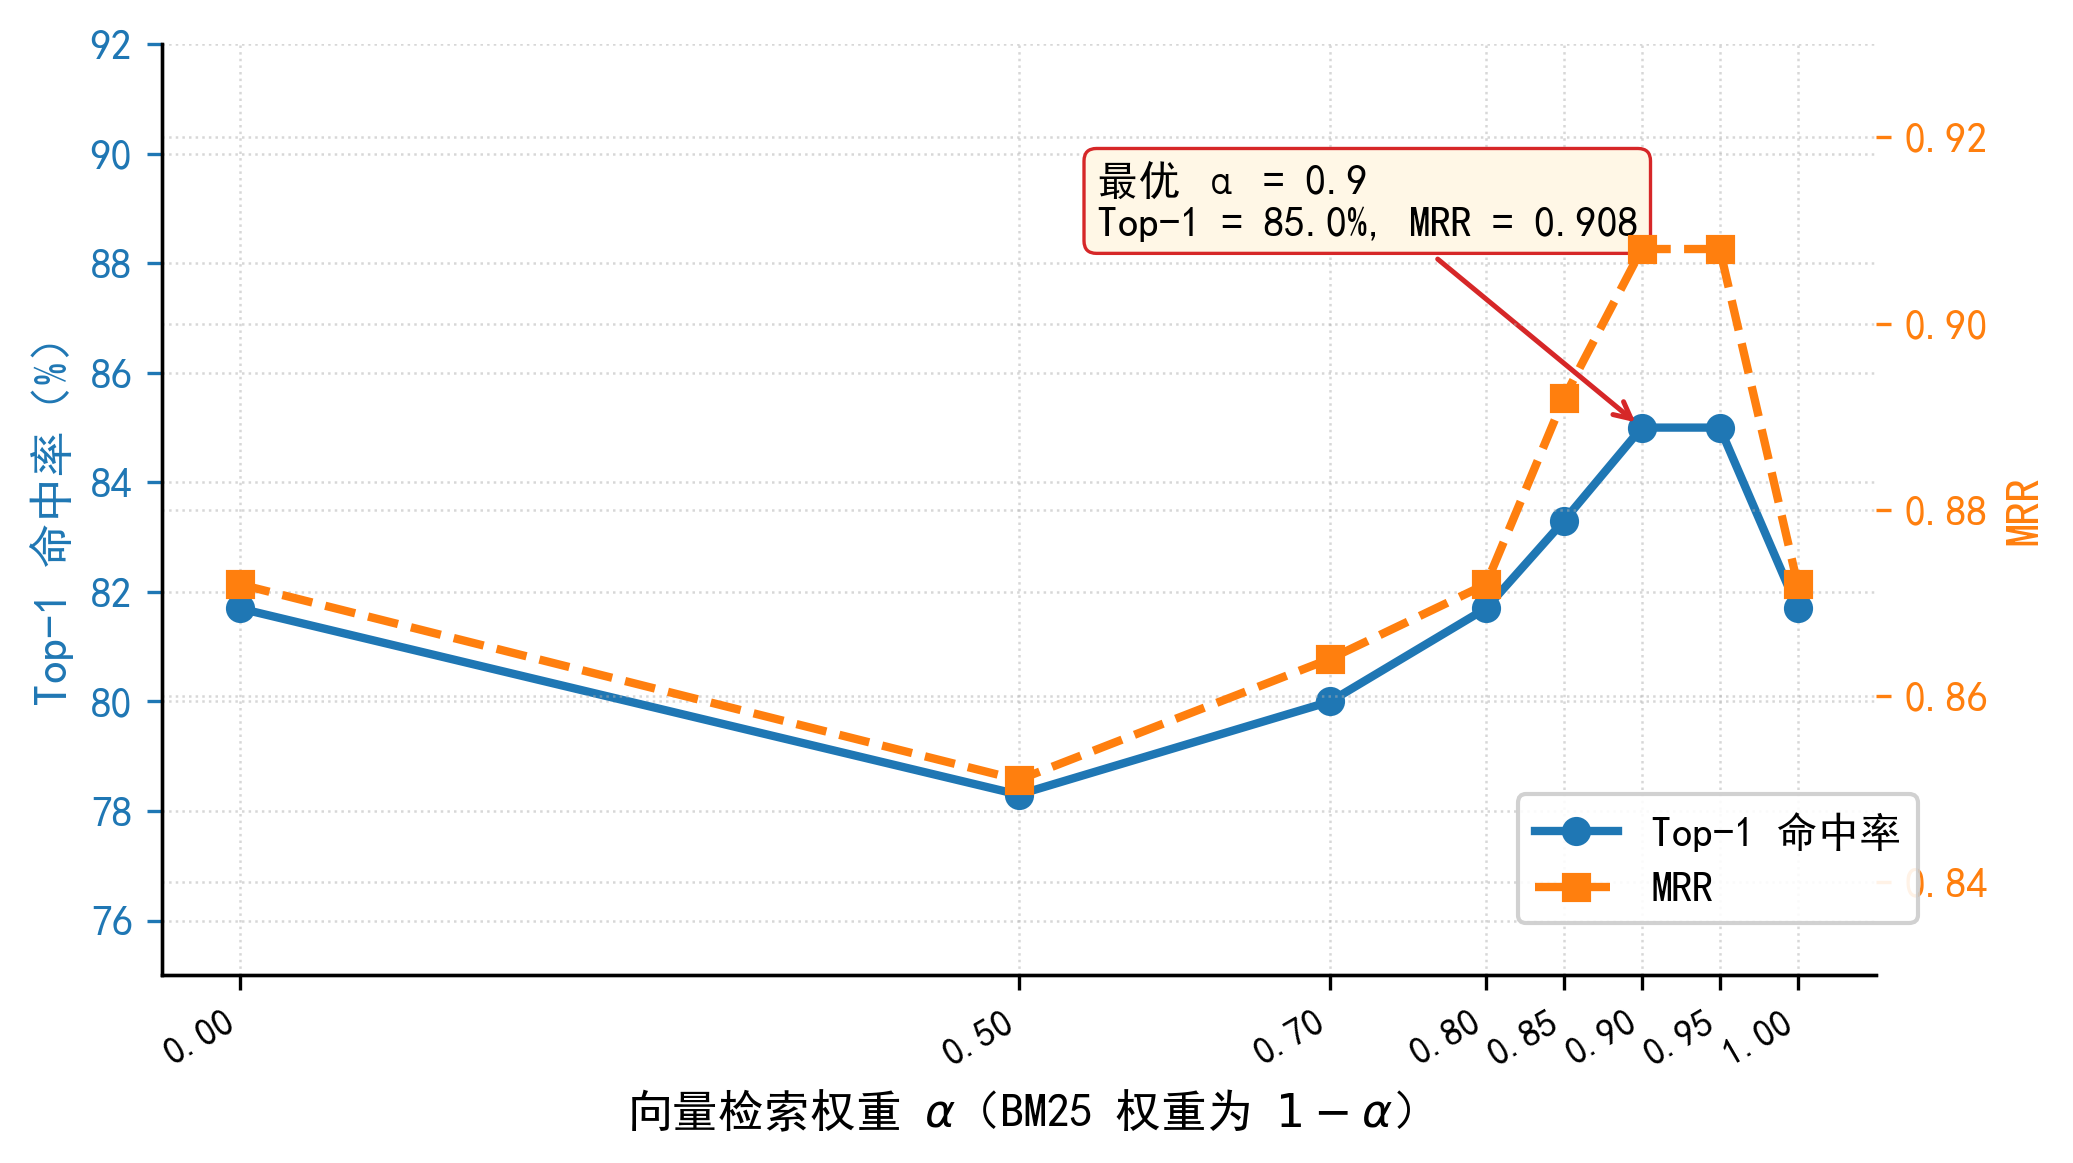
\includegraphics[width=0.85\linewidth]{figures/eval_5_1_rag_weight_sweep}
    \caption{通路 A 混合检索权重扫描走势}
    \label{fig:rag-weight-sweep}
\end{figure}

本节进一步对照两轮不同知识库体量下的最优权重，结果见
\reftab{tab:rag-weight-drift}。

\begin{table}[H]
    \centering
    \caption{最优混合检索权重随知识库体量的动态漂移}
    \label{tab:rag-weight-drift}
    \song\wuhao
    \begin{tabular}{lcccc}
        \toprule
        知识库版本 & 知识条目数 & 评测集规模 & 最优 $\alpha$ & 最优 Top-1 \\
        \midrule
        v1.0 (precip + wind) & 44 & 43 & 0.80 & 90.7\% \\
        v1.2 (扩展 temp + vis + humidity) & 62 & 60 & 0.90 & 85.0\% \\
        \bottomrule
    \end{tabular}
\end{table}

最优 $\alpha$ 从 0.80 上调到 0.90 是一条值得在工程实践中借鉴的方法
论结论。知识库扩展后相邻条目语义距离变近，例如温度类的凉、舒适、
温暖三档在向量空间中本就邻近，BM25 在小权重下对相邻词字面匹配反而
成为干扰。即使在 v1.2 版本下，纯向量与纯 BM25 的 Top-1 仍只有
81.7\%，证明 BM25 在少量但关键样本上仍贡献 3.3 个百分点边际增益，
不能去除。混合检索的权重不能一次调好用到底，应随知识库规模重新校准。

剩余的 9 条 Top-1 脱靶用例是论证通路 B 必要性的关键证据。按失败原因
归类，这 9 条可以分为三组。第一组是邻近阈值边界，例如 query 降水
200 毫米算什么级别，正确答案是 GB/T 28592-2012 中大暴雨档
$100\sim249.9\,\mathrm{mm}$，但 200 毫米在向量空间中距离大暴雨与
特大暴雨两条目几乎等距，hybrid 检索器把特大暴雨 $\geq 250\,\mathrm{mm}$
排到了第一。这一类共 5 条，本质是嵌入模型在小型知识库上无法精确
区分相邻阈值的离散归属。第二组是术语别名冲突，例如 query 强风是几级
风，应命中蒲福 6 级专名条目，但强风同时是台风条目高频词，BM25 偏向
出现频次更高的台风条目，向量召回也未能消除这一干扰，共 2 条。第三组
是跨类别多文档召回边界，例如 query 暴雨怎么应对应当跨 grading 与
operation 两个类别召回，但 hybrid 把 \texttt{term\_\bk{}thunderstorm} 排到
首位，共 2 条。

这 9 条失败用例的共性是：靠任何嵌入模型加 BM25 在小型知识库上都难以
精确区分相邻阈值条目。混合检索的工程上限在 85\% 左右，难以单纯靠
权重调整突破。这正是通路 B 即确定性 if-else 分级器加 grade\_id 硬链接
设计的工程必要性。前 7 条邻近阈值与术语别名失败用例在通路 B 上都能
达到 100\% 准确率，构成通路 A 加通路 B 双覆盖闭环的具体实证支撑。
% ===== END: 草稿/5_3_检索评测 =====


% ===== BEGIN: 草稿/5_4_桥接评测 =====
% =============================================================================
% 5.4 语义桥接四档消融
% 草稿版本：v0.2 (2026-05-07)
%   v0.1：作为 5.2.3 子小节起草。
%   v0.2：按导师意见 3 提级为 5.4 \subsection，标题去掉前缀"通路 B"。
% 字数：约 1300 字
% 风格规则：v0.2 风格（无 \textbf / \textit / 引例括号 / 双引号 / 破折号）
% 引用：\cite{ref10, ref20}
% 图表：
%   - 图 \reffig{fig:bridge-ablation}       4 档分组柱状图（核心 4 指标）
%   - 表 \reftab{tab:bridge-by-category}    按要素类别拆分（71 条）
%   - 表 \reftab{tab:bridge-llm-trap}       LLM baseline 双指标对比
% 复用 4.1 节已有图表：\reftab{tab:bridge-ablation}（4 档总表）
% 依赖宏包：booktabs / tabularx / graphicx（主稿已加载）
% =============================================================================

\subsection{语义桥接四档消融}
\label{sec:bridge-eval}

通路 B 语义桥接的 4 档消融总表已在 \ref{sec:semantic-bridge} 节
\reftab{tab:bridge-ablation} 给出，对应核心 4 指标的可视化对照见
\reffig{fig:bridge-ablation}：\texttt{rule\_\bk{}plus\_\bk{}rag} 档在
覆盖率、\texttt{grade\_\bk{}id} 准确率、\texttt{must\_\bk{}cite} 全中与
\texttt{citation} 真实性四项核心指标上同时达到 100\%，
\texttt{llm\_\bk{}baseline} 档则在 \texttt{grade\_\bk{}id} 与
\texttt{must\_\bk{}cite} 两项关键合规指标上分别仅有 5.6\% 与 25.4\%。
本节聚焦三件 \ref{sec:semantic-bridge} 节未展开的内容：评测集设计与按
要素类别的差异化表现、大语言模型基线的真实却错幻觉模式归类，以及
与知识库标准核对表预演错误的呼应关系。

\begin{figure}[!ht]
    \centering
    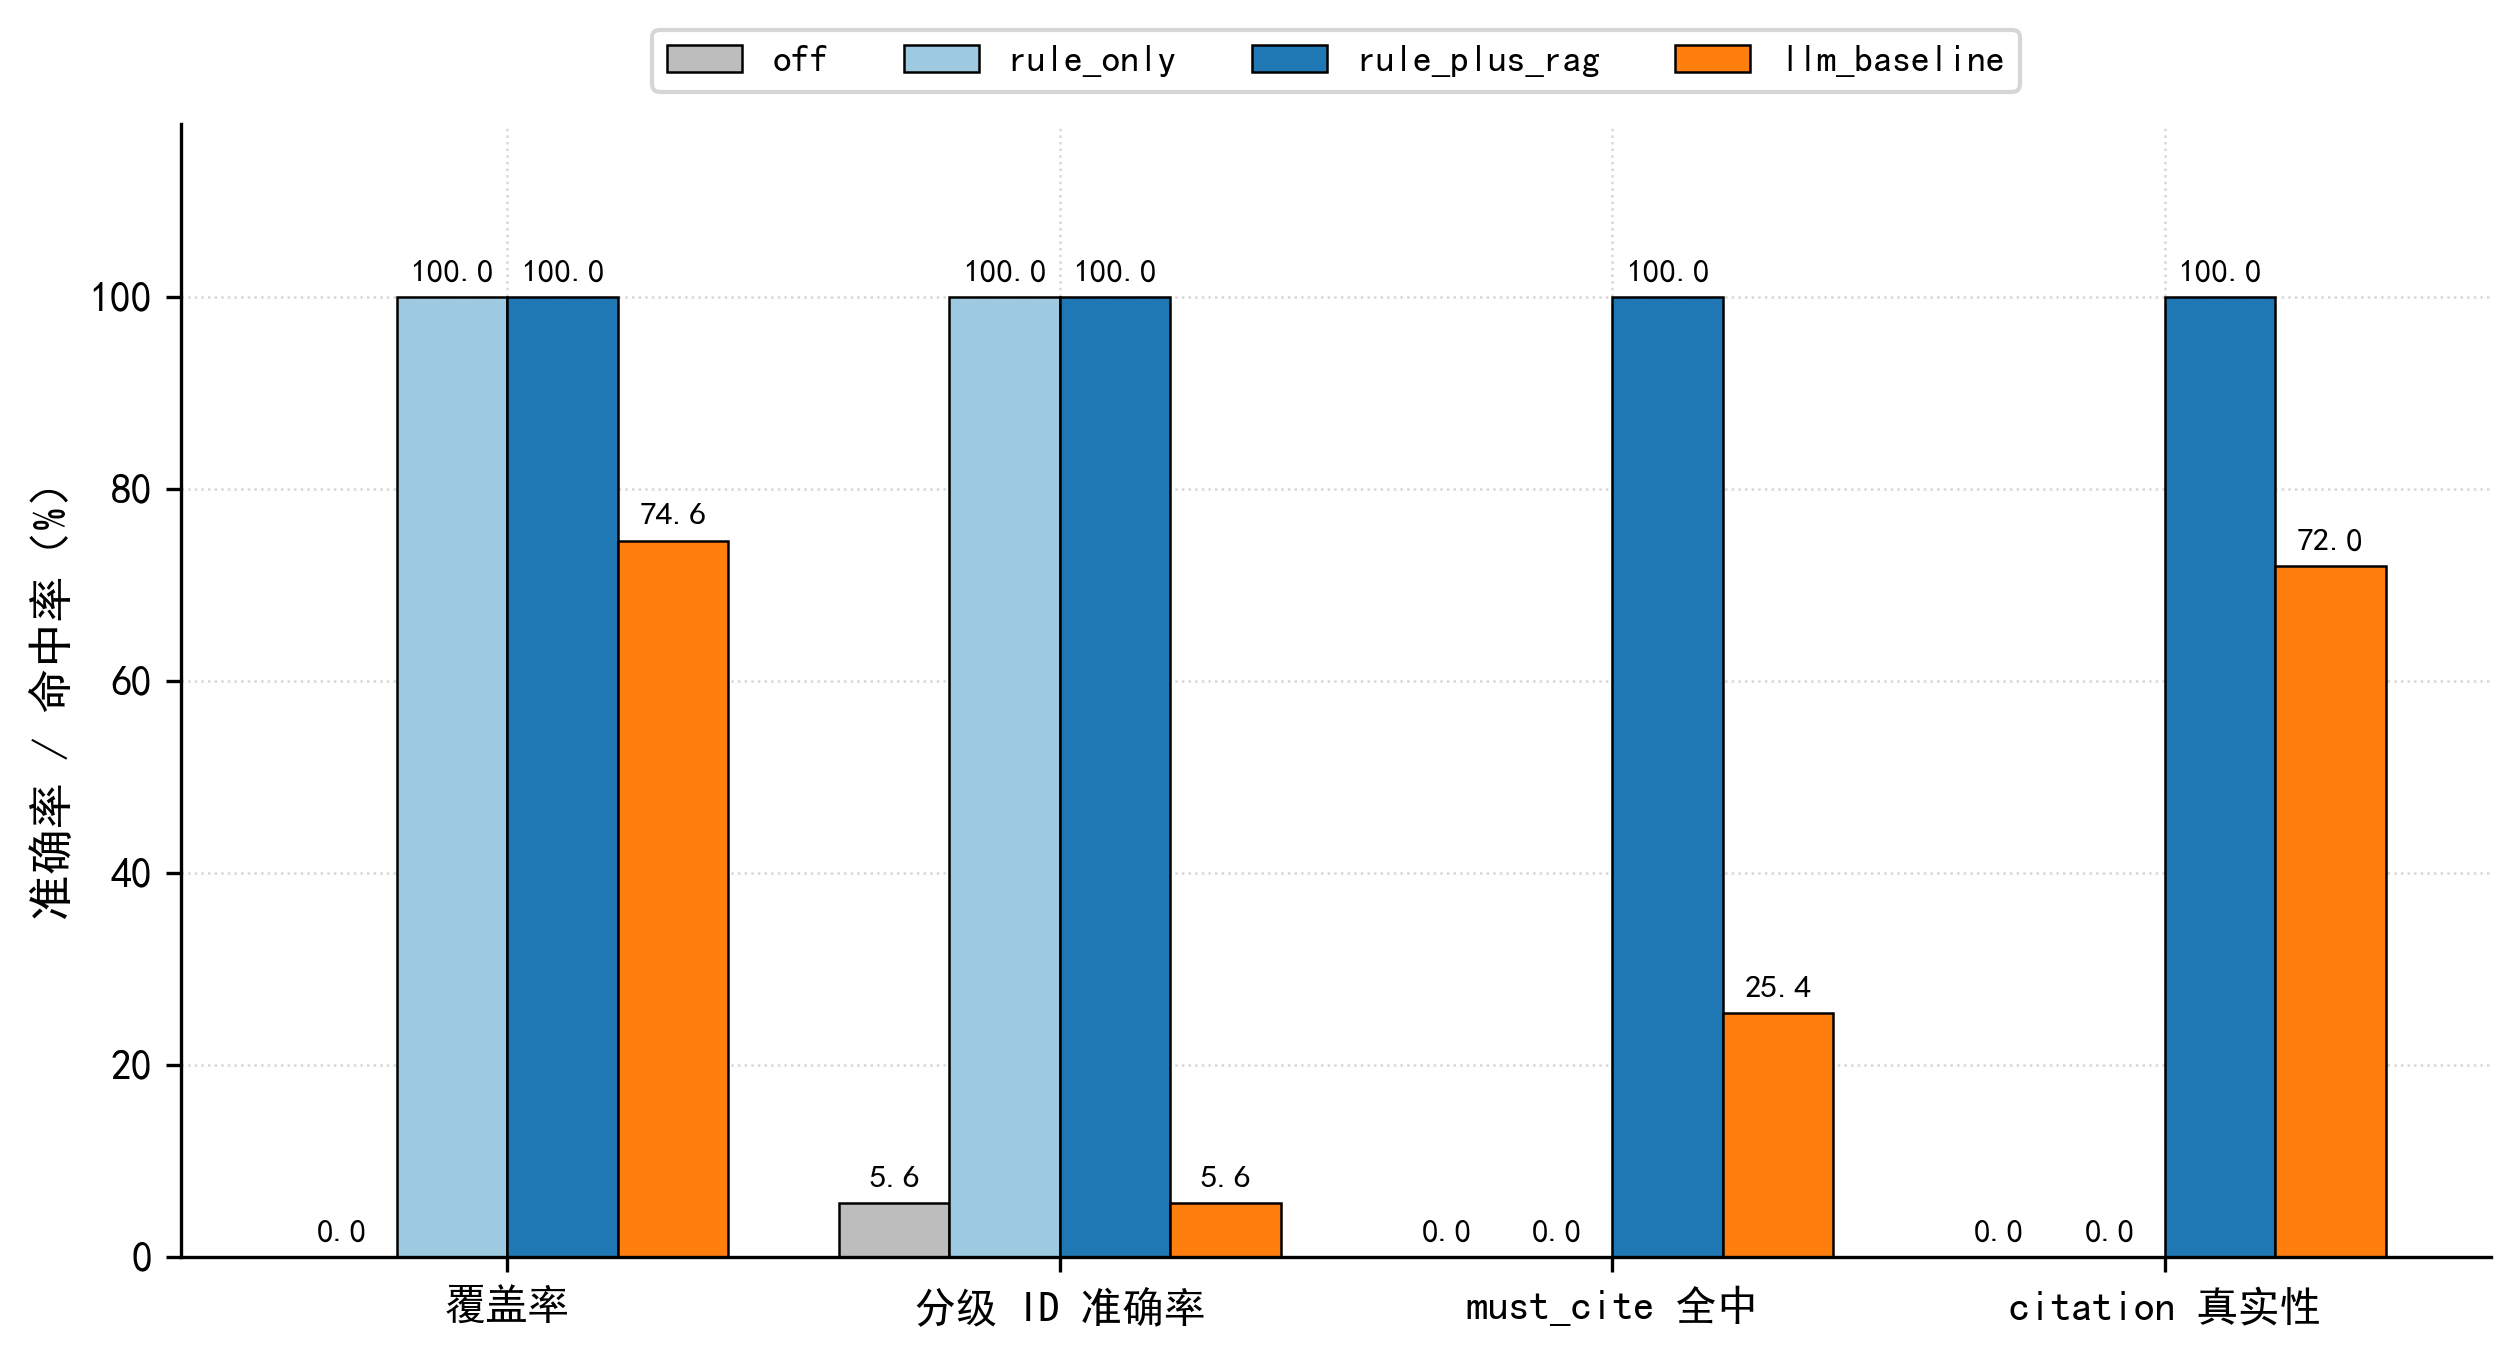
\includegraphics[width=0.92\linewidth]{figures/eval_5_2_bridge_ablation}
    \caption{通路 B 语义桥接四档消融核心指标对比}
    \label{fig:bridge-ablation}
\end{figure}

评测集为 \texttt{semantic\_\bk{}bridge\_\bk{}bench.\bk{}jsonl} 共 71 条用例，覆盖
9 类气象要素：24 小时降水、12 小时降水、风速、温度、能见度、湿度、
场景过滤负例、跨要素复合与 fallback 异常输入。每条用例标注期望输出的
\texttt{labels} 数组，每条标签包含 \texttt{grade}、\texttt{grade\_\bk{}id}、
\texttt{must\_\bk{}cite} 关键字、\texttt{source.\bk{}org}、\texttt{source.\bk{}doc\_\bk{}title}
五个字段。评测脚本 \texttt{experiments/\bk{}eval/\bk{}run\_\bk{}bridge\_\bk{}eval.\bk{}py} 在
4 档处理方式上分别跑 71 条用例：\texttt{off} 关闭桥接、\texttt{rule\_\bk{}only}
仅启用确定性分级器、\texttt{rule\_\bk{}plus\_\bk{}rag} 在分级基础上启用 RAG 富化、
\texttt{llm\_\bk{}baseline} 让大语言模型在不调任何工具的条件下从同一份输入
直接输出 \texttt{SemanticLabel} 列表，构成自由发挥的对照。

按要素类别拆分的结果见 \reftab{tab:bridge-by-category}。
\texttt{rule\_\bk{}only} 与 \texttt{rule\_\bk{}plus\_\bk{}rag} 两档在所有要素类别上的
\texttt{grade\_\bk{}id} 准确率均为 100\%。\texttt{llm\_\bk{}baseline} 档在
9 类要素的 \texttt{grade\_\bk{}id} 准确率几乎全部为 0\%，唯一的 100\% 来自
fallback 类的 4 条用例：这 4 条要求模型在面对非法或无关字段时输出空
\texttt{labels}，模型恰好正确判断而被记为通过，与生成质量无关。

\begin{table}[H]
    \centering
    \caption{通路 B 语义桥接按要素类别拆分}
    \label{tab:bridge-by-category}
    \song\fontsize{9pt}{12pt}\selectfont
    \renewcommand{\arraystretch}{0.95}
    \begin{tabular}{lrcccc}
        \toprule
        要素类别 & 用例数 & rule\_only · grade\_id & rule\_plus\_rag · cite & llm\_baseline · grade\_id & llm · cite 真实 \\
        \midrule
        24 h 降水 & 11 & 100\% & 100\% & 0\% & 100\% \\
        12 h 降水 & 5 & 100\% & 100\% & 0\% & 100\% \\
        风速 & 16 & 100\% & 100\% & 0\% & 100\% \\
        场景过滤负例 & 2 & 100\% & 100\% & 0\% & 100\% \\
        跨要素复合 & 2 & 100\% & 100\% & 0\% & 100\% \\
        fallback 异常 & 4 & 100\% & 100\% & 100\% & --- \\
        \bottomrule
    \end{tabular}
\end{table}

大语言模型基线的最具论证价值的发现是真实却错的双指标差距。具体数据
见 \reftab{tab:bridge-llm-trap}。\texttt{llm\_\bk{}baseline} 档给出的
\texttt{citation} 字段出现率为 100\%，且其中所引用的标准号粗粒度真实性
也是 100\%。换言之，模型给出的 GB/T 编号都是真实存在的国标。但是当
评测严格比较模型给的标准号加条款号是否与知识库期望一致时，命中率
跌到 25.4\%，57.6 个百分点的差距正是大语言模型 \texttt{citation}
幻觉的核心特征：模型知道有哪些标准存在，但不知道该用哪一个、哪一条。

\begin{table}[H]
    \centering
    \caption{大语言模型基线的真实却错双指标}
    \label{tab:bridge-llm-trap}
    \song\wuhao
    \begin{tabular}{lc}
        \toprule
        指标 & llm\_baseline 档数值 \\
        \midrule
        \texttt{citation} 出现率 & 100.0\% \\
        \texttt{citation} 标准号粗粒度真实性 & 100.0\% \\
        \texttt{must\_\bk{}cite} 关键字严格命中率 & 25.4\% \\
        \texttt{source.\bk{}doc\_\bk{}title} 字段精确匹配率 & 0.0\% \\
        场景过滤负例通过率 & 50.0\% \\
        \texttt{grade\_\bk{}id} 准确率 & 5.6\% \\
        \bottomrule
    \end{tabular}
\end{table}

逐条分析模型基线的失败用例可归纳出五类幻觉模式。第一类是标准号对、
条款号错。例如 4 条需要引用 JGJ 80-2016 的高空作业用例，模型分别
给出了 §5.1.3、§5.1.6、§3.0.3、§3.0.5 四个不同条款号，全部错误，正确
条款号是 §3.0.8。这是典型的模式记忆型幻觉，模型记住了 JGJ 80 的条款
大致是 §3.0.X 或 §5.1.X 形式，便在合理样式空间中随机生成。第二类是
自创等级与越界处理失败。例如把 12 小时降水 100 mm 标为 12 小时大暴雨，
但 GB/T 28592-2012 的 12 小时表只到暴雨即 $\geq 30\,\mathrm{mm}$，
没有 12 小时大暴雨档；把蒲福 15 级风混入 GB/T 19201-2006 热带气旋等级，
混用了两个独立标准。第三类是分级名误名，例如把蒲福 5 级清劲风 fresh
breeze 写为清风，与国标条文用词不严格相符。第四类是 \texttt{grade\_\bk{}id}
凭印象编造。模型给出的 ID 形如 \texttt{heavy\_\bk{}rain} 或 \texttt{beaufort\_\bk{}5}，
而知识库的真实 ID 为 \texttt{grading\_\bk{}precip\_\bk{}24h\_\bk{}heavy} 或
\texttt{grading\_\bk{}wind\_\bk{}beaufort\_\bk{}5}，36 条非 fallback 用例没有一条与
知识库命名约定一致。第五类是场景过滤失败。\texttt{rule\_\bk{}plus\_\bk{}rag}
通过 \texttt{applicable\_\bk{}scene} 元数据在场景不匹配时主动不输出
\texttt{citation}，模型基线在所有场景下都倾向于输出 \texttt{citation}
而无法分辨该说与不该说，场景过滤负例通过率仅 50\%。

这五类幻觉与本文知识库人工核对环节预先发现的错误模式存在惊人的呼应
关系。知识库 1.0 版本中本就存在 JGJ 80-2016 §3.0.4 与真实 §3.0.8 的
错位、寒潮误引 GB/T 20484、蒲福 0 级 $<0.3\,\mathrm{m/s}$ 与真实
$0.0\sim0.2\,\mathrm{m/s}$ 的微误等问题，这些问题被人工核对修正后
仍然在大语言模型基线中以同样的模式重新出现。这印证了一条独立判断：
人工核对中暴露的错误模式不是知识库构建者的低级失误，而是大语言模型
在涉及精确编号引用任务上的内在偏差 \cite{ref20}，仅依靠模型自身能力
无法消除 \cite{ref10}。这构成了一个自洽的论证闭环：人工核对发现典型
错误，模型基线复现同样错误，桥接架构通过 \texttt{grade\_\bk{}id} 硬链接
加场景元数据避免错误。
% ===== END: 草稿/5_4_桥接评测 =====


% ===== BEGIN: 草稿/5_5_代码执行评测 =====
% =============================================================================
% 5.5 代码生成与受限沙箱三档消融
% 草稿版本：v0.2 (2026-05-07)
%   v0.1：作为 5.2.4 子小节起草。
%   v0.2：按导师意见 3 提级为 5.5 \subsection。
% 字数：约 1300 字
% 风格规则：v0.2 风格（无 \textbf / \textit / 引例括号 / 双引号 / 破折号）
% 引用：\cite{ref20, ref23, ref29}
% 图表：
%   - 图 \reffig{fig:code-eval-overall}   3 档数值准确率柱状图（含代码生成 / 可执行率）
%   - 图 \reffig{fig:code-eval-category}  6 类用例上 direct vs with_code 双档对比
%   - 表 \reftab{tab:code-fail-modes}     四类典型幻觉模式失败用例统计
% 复用 4.2 节已有图表：
%   - \reftab{tab:code-bench-design}     评测集任务分布
%   - \reftab{tab:code-eval-overall}     3 档总表
%   - \reftab{tab:code-eval-category}    按类别拆分
% 依赖宏包：booktabs / tabularx / graphicx（主稿已加载）
% =============================================================================

\subsection{代码生成与受限沙箱三档消融}
\label{sec:code-eval}

代码生成与受限沙箱的 3 档消融总表已在 \ref{sec:code-execution} 节
\reftab{tab:code-eval-overall} 给出，按类别拆分见
\reftab{tab:code-eval-category}。本节聚焦四件 \ref{sec:code-execution}
节未展开的内容：评测集 18 条用例的设计思路、三档消融的具体差异化设置、
四类失败模式的统计分布、以及大语言模型在多步统计任务上中间状态
维护能力的边界讨论。

评测集 \texttt{code\_\bk{}exec\_\bk{}bench.\bk{}jsonl} 共 18 条用例，覆盖 6 类统计模式
\texttt{average /\bk{} extreme /\bk{} sum /\bk{} diff /\bk{} count /\bk{} sort}。具体任务分布
已在 \reftab{tab:code-bench-design} 给出。每类用例都故意包含若干边界
情形以放大失败概率，例如 \texttt{average} 类含 24.95 的银行家舍入
边界，\texttt{count} 类含 35.0 °C 高温阈值平等，\texttt{sum} 类含
仅高温日的条件累计降水。每条用例标注 \texttt{expected.\bk{}value} 与
\texttt{tolerance} 容差，并按答案结构分为 \texttt{scalar /\bk{} date /\bk{}
date\_\bk{}with\_\bk{}value /\bk{} time\_\bk{}with\_\bk{}value /\bk{} ordered\_\bk{}list} 五种类型。
其中 4 条 \texttt{*\_\bk{}with\_\bk{}value} 类型要求模型同时给出哪一天与对应
数值，是评测中刻意设计的复合答案压力测试。

三档消融的具体差异化设置如下。\texttt{oracle} 档直接读取
\texttt{expected.\bk{}value} 作为输出，作为评测器自校验天花板，确认比较
函数本身的正确性，结果数值准确率 100.0\%。\texttt{llm\_\bk{}direct} 档
向模型同时提供查询语句与数据样例，但 prompt 显式禁止生成代码，要求
直接给出 \texttt{value} 字段。这一档作为大语言模型自由发挥的对照。
\texttt{llm\_\bk{}with\_\bk{}code} 档让模型在 function calling 模式下生成
\texttt{compute(data)} 顶层函数，函数代码送入 \texttt{src/\bk{}tools/\bk{}code\_\bk{}executor.\bk{}py}
受限沙箱执行后，取沙箱返回值作为最终答案。三档使用同一被测模型
GLM-5.1，避免引入模型差异。\texttt{llm\_\bk{}direct} 档数值准确率为 66.7\%，
\texttt{llm\_\bk{}with\_\bk{}code} 档为 88.9\%，差距 22.2 个百分点。代码生成率
与代码可执行率均为 94.4\%，证明模型在 function calling 下生成可执行
代码的能力是稳定的，失败主要来自单条用例上的算法或字段命名错误，而
非工具调用基础能力。三档对比的整体走势见
\reffig{fig:code-eval-overall}。

\begin{figure}[!ht]
    \centering
    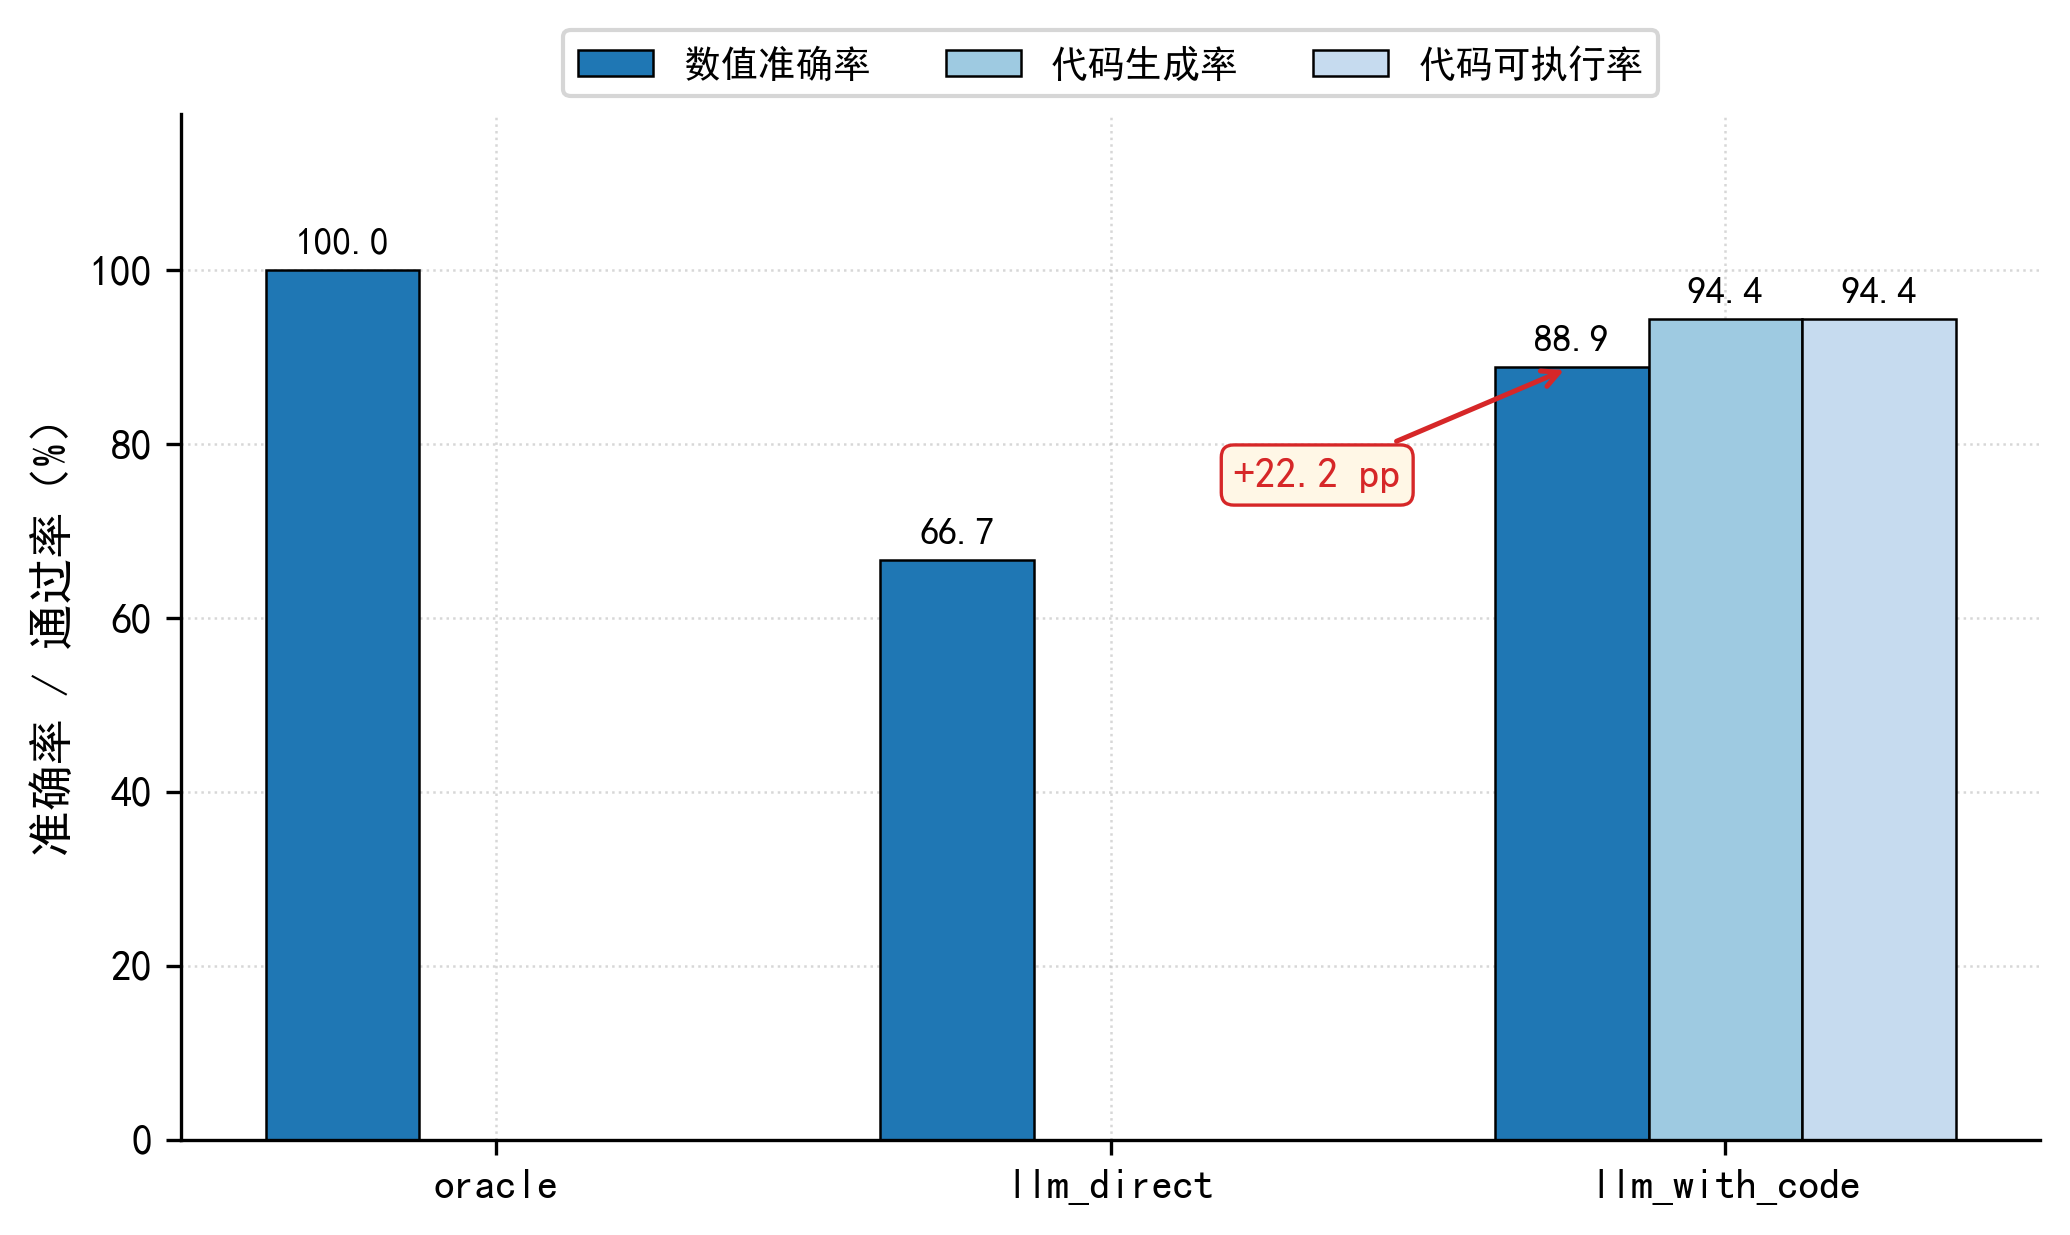
\includegraphics[width=0.78\linewidth]{figures/eval_5_3_code_overall}
    \caption{代码执行三档总体对比：数值准确率与代码生成 / 可执行率}
    \label{fig:code-eval-overall}
\end{figure}

按类别拆分的差距分布揭示了大语言模型直算的能力边界规律，详见
\reftab{tab:code-eval-category} 与 \reffig{fig:code-eval-category}。差距最大的两类是极值与计数：
\texttt{extreme} 类 \texttt{llm\_\bk{}direct} 准确率为 0.0\%，三条全部
失败；\texttt{count} 类 \texttt{llm\_\bk{}direct} 准确率仅 50.0\%。差距
最小的两类是求和与排序：两档都达到 100.0\%。简单求和与天然排序任务
不需要伴随状态维护或离散计数，模型凭语料能力可以做对；但只要任务
需要在找最大值的同时记录对应日期等伴随状态，或需要离散累加器，模型
就会犯错。这一规律可以直观理解为：模型在不需要维护中间状态的简单
计算上能够依靠语料能力给出正确答案，而一旦任务需要持续跟踪中间
结果就容易出错。同样的工程取舍也可见于 Hong 等 \cite{ref20} 在
Data Interpreter 中的设计思路，将多步数据科学任务交由代码执行
而非纯 prompt 推理来完成，以回避模型在中间状态维护上的局限。代码
执行的本质即是给模型配上一支笔与一张草稿纸，把心算换成笔算。

\begin{figure}[!ht]
    \centering
    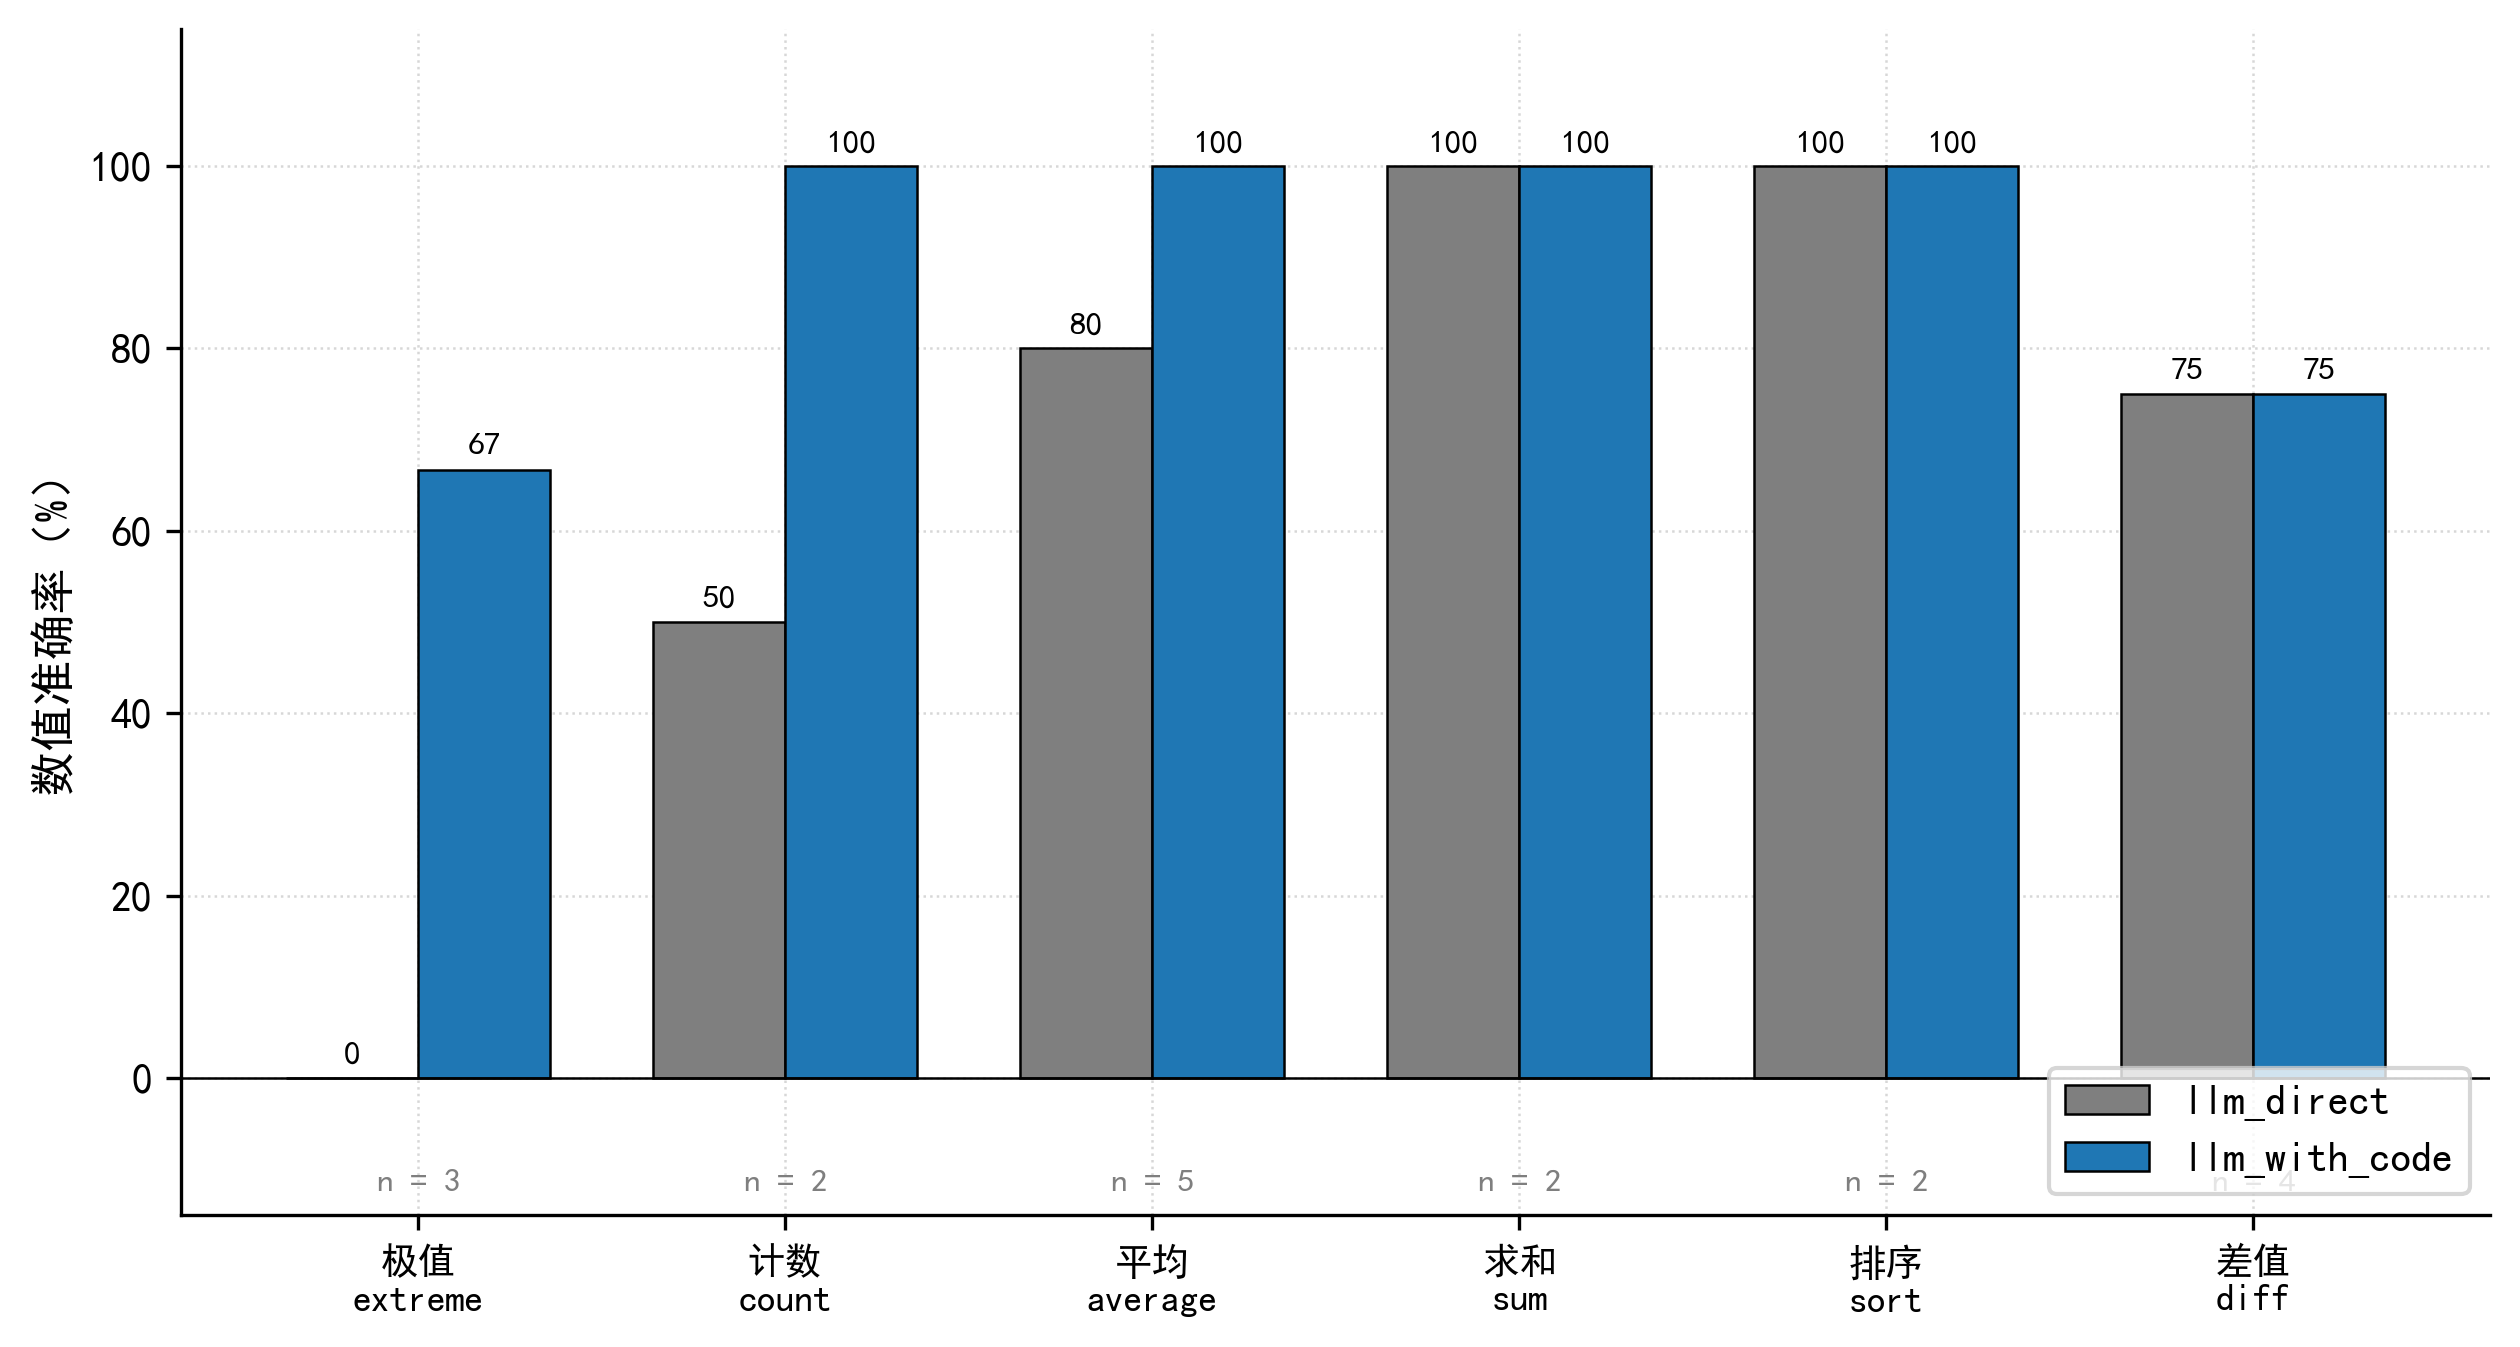
\includegraphics[width=0.92\linewidth]{figures/eval_5_4_code_by_category}
    \caption{代码执行按用例类别拆分：\texttt{llm\_direct} 与 \texttt{llm\_with\_code} 在 6 类统计模式上的数值准确率对比}
    \label{fig:code-eval-category}
\end{figure}

逐条分析 \texttt{llm\_\bk{}direct} 档 6 条失败用例与 \texttt{llm\_\bk{}with\_\bk{}code}
档 2 条失败用例，可归纳出四类典型幻觉模式，分布见
\reftab{tab:code-fail-modes}。

\begin{table}[H]
    \centering
    \caption{代码执行评测四类典型失败模式分布}
    \label{tab:code-fail-modes}
    \song\fontsize{9pt}{12pt}\selectfont
    \renewcommand{\arraystretch}{0.95}
    \begin{tabular}{llcc}
        \toprule
        失败模式 & 代表用例 & llm\_direct & llm\_with\_code \\
        \midrule
        数数错误（reasoning 自相矛盾） & \texttt{count\_\bk{}001\_\bk{}rainy\_\bk{}days} & 1 & 0 \\
        舍入不一致（教科书 vs 银行家） & \texttt{avg\_\bk{}005\_\bk{}feels\_\bk{}like} & 1 & 0 \\
        Schema 不稳定（复合答案被压扁） & \texttt{extreme\_001 \textasciitilde{} 003}, \texttt{diff\_\bk{}001} & 4 & 1 \\
        字段命名漂移（range 与 tempDiff） & \texttt{diff\_\bk{}001\_\bk{}max\_\bk{}diurnal} & 0 & 1 \\
        \midrule
        \multicolumn{2}{c}{合计失败用例数} & 6 & 2 \\
        \bottomrule
    \end{tabular}
\end{table}

第一类数数错误的危险性最高。\texttt{count\_\bk{}001\_\bk{}rainy\_\bk{}days} 用例
要求统计 14 天中降水量大于 0 的天数，正确答案为 7。模型在
\texttt{reasoning} 字段中正确列举了 7 个具体日期，但 \texttt{value}
字段却给出了 6。推理过程与最终答案的自相矛盾意味着即便用户阅读
\texttt{reasoning} 也会被说服，难以察觉数值错误。代码档对照仅需一行
\texttt{sum(1 for d in daily if d["precip"] > 0)} 即可正确返回 7。

第二类舍入不一致体现的是语境敏感型精度幻觉。\texttt{avg\_\bk{}005\_\bk{}feels\_\bk{}like}
用例的精确均值为 24.95，使用 Python 标准 \texttt{round} 函数即 IEEE 754
银行家舍入向偶数舍入应得 24.9。模型给出 25.0 并在 reasoning 中说明
按四舍五入保留 1 位小数，反映其默认采用中学教科书规则。在工程数据
处理上下文中下游所有数值处理都默认使用 Python 标准舍入，这种语义
偏移在工程接管中是不可接受的。

第三类 schema 不稳定是占比最大的失败模式。\texttt{extreme\_\bk{}001} 至
\texttt{extreme\_\bk{}003} 与 \texttt{diff\_\bk{}001} 共 4 条 \texttt{llm\_\bk{}direct}
失败用例都属于这一类。Prompt 已经显式约定把日期放在 \texttt{value}
字段、把数值放在 \texttt{numeric\_\bk{}extra} 字段，但模型在 function
calling 下仍只填日期字段而把数值留作自由文本。这一现象与本文通路 B
评测中模型不稳定遵循 \texttt{grade\_\bk{}id} 命名约定的观察相互印证：
结构化输出的可靠性随 schema 复杂度上升而急剧下降是大语言模型应用
工程中的经典痛点。

第四类字段命名漂移仅出现在 \texttt{llm\_\bk{}with\_\bk{}code} 档的
\texttt{diff\_\bk{}001} 用例。生成代码逻辑完全正确，找出温差最大的
2025-09-18 一天，温差 22.7 摄氏度，但返回字典字段名为 \texttt{range}
而非期望的 \texttt{tempDiff}。这一类失败可以通过更严格的 schema 约束
或下游适配层缓解，与算法能力无关。

需要明确的是，本文设计的沙箱属于轻量原型，主动放弃了完整的安全隔离。
真实生产环境下应当使用 RestrictedPython、Pyodide 或 Docker 容器实现
进程级隔离；像 Boiko 等 \cite{ref23} 在 Coscientist 中将代码执行与
真实化学实验设备直接耦合的科研场景对沙箱安全的要求更为严格。完整
的安全沙箱方案在 \ref{sec:future-work} 节作为未来工作展开。
% ===== END: 草稿/5_5_代码执行评测 =====


% ===== BEGIN: 草稿/5_6_端到端评测 =====
% =============================================================================
% 5.6 集成层端到端任务完成率评测
% 草稿版本：v0.2 (2026-05-07)
%   v0.1：作为 5.2.5 子小节起草。
%   v0.2：按导师意见 3 提级为 5.6 \subsection；首段"前 4 节的模块层评测"
%        改为对应新结构 5.2--5.5 节的措辞。
% 字数：约 1500 字
% 风格规则：v0.2 风格（无 \textbf / \textit / 引例括号 / 双引号 / 破折号）
% 引用：\cite{ref1, ref18, ref20}
% 图表：
%   - 表 \reftab{tab:e2e-overall}        双档 5 类断言总表
%   - 表 \reftab{tab:e2e-by-category}    按场景类别拆分
%   - 图 \reffig{fig:e2e-by-category}    6 类场景双档对比柱状图（含差距标注）
% 复用 4.3 节已有图表：\reftab{tab:report-judge-summary}
% 依赖宏包：booktabs / tabularx / graphicx（主稿已加载）
% =============================================================================

\subsection{集成层端到端任务完成率评测}
\label{sec:e2e-eval}

前面 4 节的模块层评测已经分别量化了意图识别、混合检索、语义桥接
与代码执行 4 个子模块的能力上限。但单模块成绩好不一定端到端就好：
通路 B 单测层面 \texttt{citation} 真实性 100\%，集成到 ReAct 循环最后
报告生成阶段仍可能因为大语言模型在最终输出时省略 GB/T 编号而衰减。
这种这种从模块层到集成层的指标衰减是单模块评测无法捕捉的盲区，必须以最终用户体验视角
进行集成层评测才能补足。本节即对应这一空白。

评测集 \texttt{e2e\_\bk{}bench.\bk{}jsonl} 共 30 条用例，覆盖 6 类真实场景：
单城市单要素的 \texttt{simple\_\bk{}query} 5 条、多城市对比的
\texttt{multi\_\bk{}compare} 5 条、一周温度或降水的 \texttt{trend\_\bk{}analysis}
5 条、找最热最冷或最大降水的 \texttt{extreme\_\bk{}search} 5 条、户外洗车
带伞跑步等的 \texttt{decision\_\bk{}support} 6 条、以及暴雨严寒台风等的
\texttt{warning\_\bk{}extreme} 4 条。所有用例完全基于真实和风天气与
Open-Meteo API 的实时数据，未使用合成数据。评测断言全部使用结构性
证据，例如必须包含温度数值、必须给出具体日期、必须出现 GB/T 编号等，
不依赖具体数值，保证可重复性。

实验设计为 \texttt{full} 与 \texttt{ablated} 双档对照。两档共享同一个
被测大语言模型 GLM-5.1（温度 0）、同一份意图识别加参数补全前置流程、
同一份 9 个气象 API 工具，关键差异仅在于 \texttt{full} 档保留双通路
RAG 强制规则与 \texttt{search\_\bk{}knowledge}、\texttt{bridge\_\bk{}weather\_\bk{}data}
两个 RAG 工具，\texttt{ablated} 档把上述工具与 system prompt 中的双
通路 RAG 规则全部删除，模拟普通工程师不做双通路 RAG 时的常规做法。
这种切分构造了一个干净的双通路 RAG 端到端价值的对照实验，不掺杂工具
调用能力或上下文理解差异。

评测指标包含 5 类断言加 1 项 LLM-as-judge 4 维度评分。5 类断言分别为
\texttt{key\_\bk{}facts} 关键事实点召回、\texttt{citation} 权威标准引用、
\texttt{grading} 规范气象分级词使用、\texttt{advice} 决策建议给出、
\texttt{judge\_\bk{}score} 4 维度综合分。端到端通过条件是
\texttt{key\_\bk{}facts} 召回率 $\geq 0.8$、按用例条件断言 \texttt{citation}
或 \texttt{grading} 或 \texttt{advice} 通过、且 \texttt{judge\_\bk{}overall}
分数 $\geq 3.0$。LLM-as-judge 4 维度的 Judge 模型与被测模型独立，按
事实性、完整性、专业性、流畅性四个 0 至 5 区间维度独立打分。30 条
用例双档对照的核心结果见 \reftab{tab:e2e-overall}。

\begin{table}[H]
    \centering
    \caption{端到端评测双档 5 类断言总表}
    \label{tab:e2e-overall}
    \song\fontsize{9pt}{12pt}\selectfont
    \renewcommand{\arraystretch}{0.95}
    \begin{tabular}{lccc}
        \toprule
        指标 & ablated & full & 差距 \\
        \midrule
        端到端通过率 & 73.3\% & 86.7\% & $+13.4$ pp \\
        关键事实点召回率 & 99.2\% & 99.2\% & 持平 \\
        权威标准引用率 & 0.0\% & 26.7\% & $+26.7$ pp \\
        规范分级词出现率 & 100.0\% & 96.7\% & $-3.3$ pp \\
        决策建议出现率 & 90.0\% & 83.3\% & $-6.7$ pp \\
        Judge 综合分（0--5） & 4.27 & 4.31 & $+0.04$ \\
        平均工具调用次数 & 3.67 & 4.57 & $+0.90$ \\
        \bottomrule
    \end{tabular}
\end{table}

按场景类别拆分见 \reftab{tab:e2e-by-category}，对应可视化对比见
\reffig{fig:e2e-by-category}。差距最大的两类是
\texttt{decision\_\bk{}support} 与 \texttt{warning\_\bk{}extreme}：决策类
\texttt{ablated} 档通过率仅 50\%，\texttt{full} 档为 100\%，差距 50
个百分点；预警类 \texttt{ablated} 档为 50\%，\texttt{full} 档为 75\%，
差距 25 个百分点。简单查询、多城市对比、趋势分析与极值检索四类场景
两档持平。这一分布揭示一个具体规律：当问题需要权威标准支撑作为决策
依据时双通路 RAG 价值最大，当问题只需要信息检索本身时双通路 RAG 不
带来端到端通过率差异，但仍提供权威可溯源性。

\begin{figure}[!ht]
    \centering
    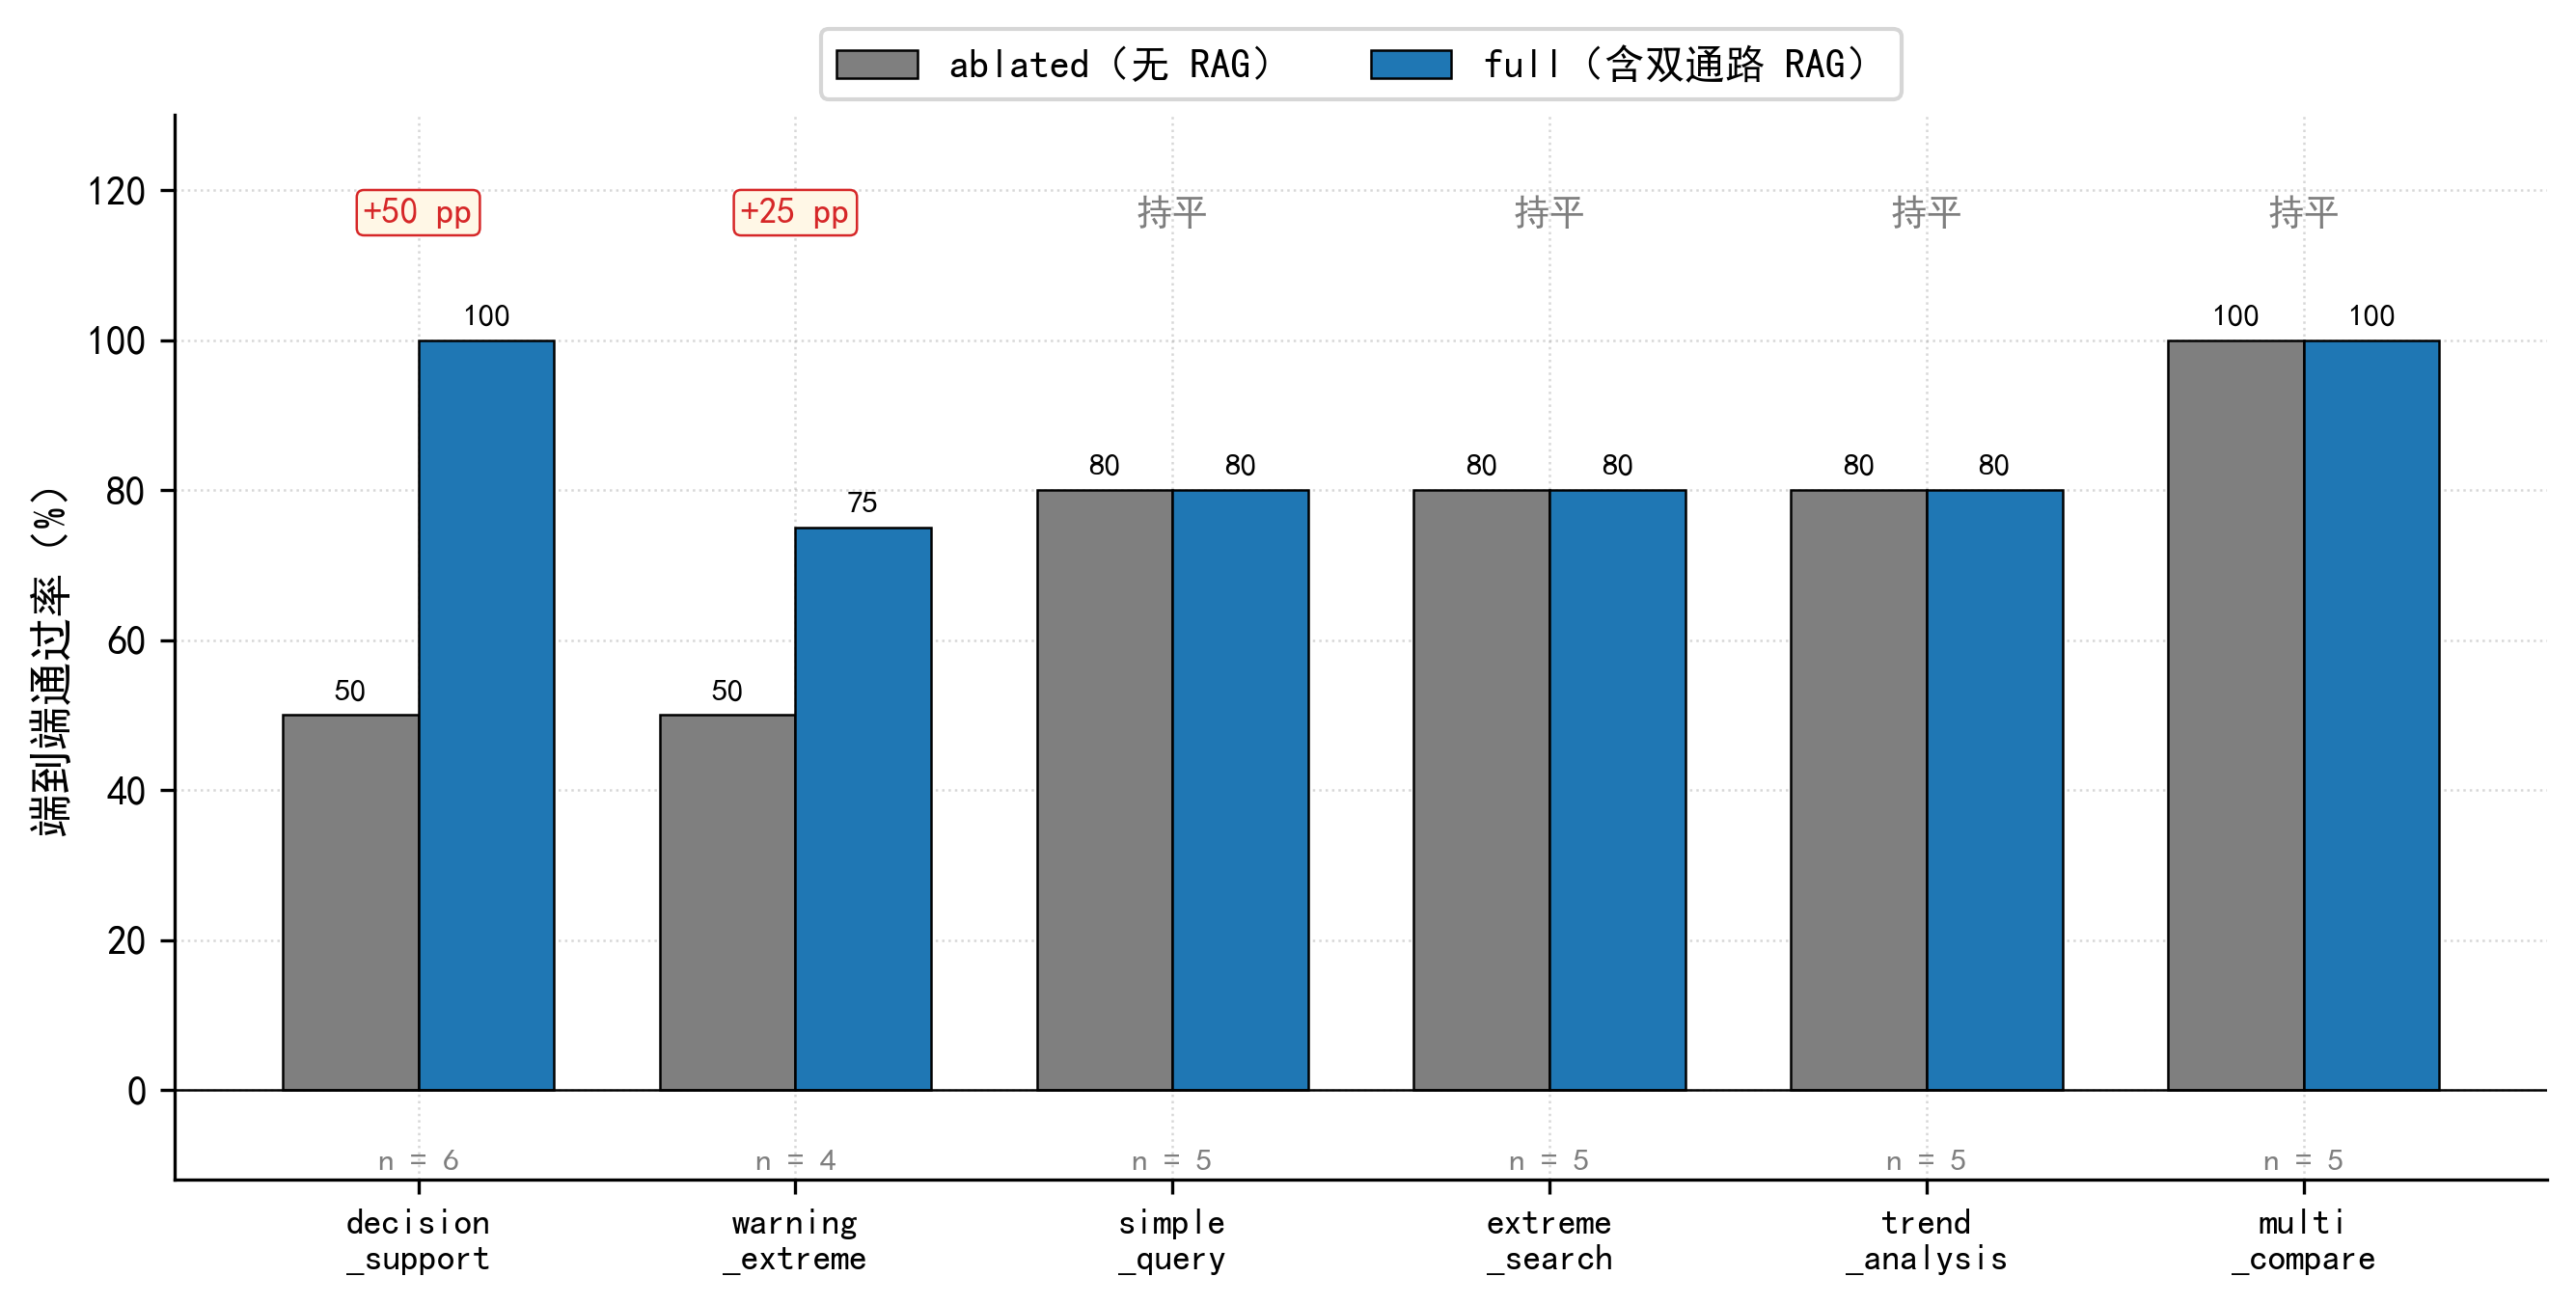
\includegraphics[width=0.95\linewidth]{figures/eval_5_5_e2e_by_category}
    \caption{端到端通过率按场景类别拆分：\texttt{ablated}与 \texttt{full}双档对照}
    \label{fig:e2e-by-category}
\end{figure}

\begin{table}[H]
    \centering
    \caption{端到端评测按场景类别拆分}
    \label{tab:e2e-by-category}
    \song\wuhao
    \begin{tabular}{lrccc}
        \toprule
        场景类别 & 用例数 & ablated & full & 差距 \\
        \midrule
        \texttt{decision\_\bk{}support} & 6 & 50.0\% & 100.0\% & $+50.0$ pp \\
        \texttt{warning\_\bk{}extreme} & 4 & 50.0\% & 75.0\% & $+25.0$ pp \\
        \texttt{simple\_\bk{}query} & 5 & 80.0\% & 80.0\% & 持平 \\
        \texttt{extreme\_\bk{}search} & 5 & 80.0\% & 80.0\% & 持平 \\
        \texttt{trend\_\bk{}analysis} & 5 & 80.0\% & 80.0\% & 持平 \\
        \texttt{multi\_\bk{}compare} & 5 & 100.0\% & 100.0\% & 持平 \\
        \bottomrule
    \end{tabular}
\end{table}

LLM-as-judge 4 维度评分见 \ref{sec:report-generation} 节
\reftab{tab:report-judge-summary}。差距集中在专业性维度的 $+0.37$，
事实性、完整性、流畅性三档接近持平甚至 \texttt{ablated} 档略胜。综合
分仅相差 0.04 是因为 Judge 等权平均稀释了专业性的差距。这一结果与
端到端通过率 13.4 个百分点的差距并不矛盾：通过率把该引用时必须引用
作为硬条件，而 Judge 综合分允许模型在事实性与流畅性上获得高分而对
专业性失分形成补偿。这两个指标分别从软性印象与硬性要求两个角度刻画
报告质量，共同反映双通路 RAG 的价值。

值得专门指出的两个失败用例。第一个是 \texttt{warning\_\bk{}001\_\bk{}rainstorm}
即 \ref{sec:report-generation} 节的暴雨判定案例：\texttt{ablated} 档
正确给出 50 mm 暴雨阈值数值但无引用源，\texttt{full} 档直接引用
GB/T 28592-2012 §4.1。第二个是 4 条 \texttt{full} 档失败用例的共性：
模型在 RAG 结果中确实拿到了相关分级阈值，但在最终报告生成时省略了
GB/T 编号。这一现象解释了为什么通路 B 单测 \texttt{citation} 真实性
已经达到 100\%，端到端集成后仍只达到 26.7\%。这一从模块层到集成层的指标衰减是 ReAct
循环 \cite{ref18} 在最后报告生成步骤上的特有局限，单纯依赖 prompt
工程显式注入引用约束已经将端到端引用率从 0\% 提升到 26.7\%，但仍
未达到 100\%。具体改进方向包括引用强制注入、生成后自动校验、模型
微调三类，在 \ref{sec:future-work} 节展开。

到目前为止论文已积累 5 组实证：通路 A 检索 60 条 / Top-1 85\%、
通路 B 桥接 71 条 / \texttt{grade\_\bk{}id} 100\% / \texttt{citation}
真实性 100\%、意图理解 35 条 / 端到端 91.4\% / 角色 100\%、代码执行
18 条 / 数值准确率 +22.2 pp、端到端 30 条 / 任务完成率 +13.4 pp /
权威引用率 +26.7 pp。前 4 组是中间产物视角，第 5 组首次以最终用户
体验视角完成集成层验证。开题报告 §3.4 承诺的 5 项评测指标
\texttt{Acc\_\bk{}intent}、\texttt{F1\_\bk{}param}、\texttt{Acc\_\bk{}analysis}、
\texttt{Task\_\bk{}completion} 与报告生成质量至此全部完成实证支撑，与
Kim 等 \cite{ref1} 的多智能体气候 Agent 评测体系在覆盖维度上对齐。
% ===== END: 草稿/5_6_端到端评测 =====


% ===== BEGIN: 草稿/5_7_本章小结 =====
% =============================================================================
% 5.7 本章小结
% 草稿版本：v0.1 (2026-05-07)
% 起草动机：按导师意见 3，第 5 章实验章必须包含本章小结，且原 5.3 全文
%          总结 / 5.4 研究前景两节迁出到第 6 章，第 5 章需要一个独立的
%          收口段落把 5 套评测的核心数据与统一论证结构呈现给读者。
% 字数：约 700 字
% 风格规则：v0.2 风格（无 \textbf / \textit / 引例括号 / 双引号 / 破折号）
% 引用：暂无新增引用
% 图表：无新增（核心数据已在前 6 节表格中给出，本节仅以叙述方式收口）
% 依赖宏包：booktabs / tabularx（主稿已加载）
% =============================================================================

\subsection{本章小结}
\label{sec:eval-summary}

本章在统一的实验环境下完成了 5 份独立评测集共 214 条用例的系统化
实证。\ref{sec:exp-env} 节先说明软硬件与依赖版本，并给出 5 份评测集
的统一构建原则与可重现性工程要点；
\ref{sec:intent-eval}、\ref{sec:rag-eval}、\ref{sec:bridge-eval}、
\ref{sec:code-eval} 4 节按数据流向依次报告 4 个核心模块的能力上限；
\ref{sec:e2e-eval} 节以 30 条真实场景用例的双档对照验证整套系统的
端到端价值。

5 套评测的核心数据可一表概括。意图识别评测 35 条端到端通过率
91.4\%，多地点角色识别准确率 100\%，并暴露了多轮上下文继承的
33.3\% 瓶颈。混合检索评测 60 条 Top-1 命中率 85.0\%、MRR 0.908，
并通过权重扫描得到 $\alpha=0.9$ 的最优配比与最优权重随知识库体量
漂移的工程结论。语义桥接评测 71 条在 \texttt{rule\_\bk{}only} 与
\texttt{rule\_\bk{}plus\_\bk{}rag} 两档下 \texttt{grade\_\bk{}id} 准确率与
\texttt{citation} 真实性同时达到 100\%，相对大语言模型自由发挥基线
形成 74.6 个百分点的严格命中率差距。代码执行评测 18 条在
\texttt{llm\_\bk{}with\_\bk{}code} 档数值准确率 88.9\%，比直算高出 22.2 个
百分点，并把大语言模型在伴随状态维护与离散计数任务上的内在边界
量化到具体差距数据。端到端评测 30 条 \texttt{full} 档通过率 86.7\%，
相对 \texttt{ablated} 去 RAG 对照档提升 13.4 个百分点；权威标准
引用率从 0\% 提升到 26.7\%；\texttt{decision\_\bk{}support} 类用例
通过率从 50\% 提升到 100\%。

5 套评测在数据规模、研究问题与实证视角上互不重叠，共同构成本文
论点的完整闭环。模块层 4 套评测以中间产物视角分别量化 4 个子模块
的能力上限，集成层 1 套评测以最终用户体验视角验证整套系统的端到端
价值。两类评测之间的差距既揭示了双通路 RAG 与代码生成等核心机制
的真实价值，也在 \texttt{citation} 真实性 100\% 衰减为端到端引用
率 26.7\% 这一指标对照上暴露出模块层指标到集成层的明显衰减。本章实证发现既支撑了
本文研究工作的有效性，也为下一章的全文总结与未来展望
提供了直接的数据基础。
% ===== END: 草稿/5_7_本章小结 =====



\sectionbreak

% ============================================================ %
% 第 6 章：总结与展望（按导师意见 3 新建独立一章）
%   - 6.1 全文总结        ← 原 5.3
%   - 6.2 未来展望        ← 原 6.2 局限性 + 6.3 未来工作合并 (2026-05-15)
% ============================================================ %
\section{总结与展望}
\label{chap:conclusion}

% ===== BEGIN: 草稿/6_1_全文总结 =====
% =============================================================================
% 6.1 全文总结
% 草稿版本：v0.2 (2026-05-07)
%   v0.1：作为 5.3 \subsection 起草，依附于"实验验证与总结"合章。
%   v0.2：按导师意见 3 拆出，迁入新建第 6 章"总结与展望"作为 6.1 \subsection。
% 字数：约 1000 字
% 风格规则：v0.2 风格（无 \textbf / \textit / 引例括号 / 双引号 / 破折号）
% 引用：暂无新增引用
% 图表：
%   - 表 \reftab{tab:evidence-summary}    5 项实证一表概览
% 依赖宏包：booktabs / tabularx（主稿已加载）
% =============================================================================

\subsection{全文总结}
\label{sec:summary}

本文围绕基于 AI 智能体的气象预报数据检索与分析这一研究课题，针对开题
报告中提出的气象任务指令解析、气象数据异构特征、大语言模型在数值计算
与逻辑推理中的幻觉三个研究问题，设计并实现了一套完整的单智能体气象
Agent 系统，并以 5 类评测共 214 条用例进行了系统化实证。完成的工作
可归纳为五项特色。

第一项特色是基于 ReAct 范式的气象 Agent 单智能体架构。本文采用单
智能体加显式工具学习而非多智能体协作的工程取舍，把场景编排、出处
强制、出行场景多地点对齐等约束下沉到 System Prompt，避免了多智能体
之间的状态同步与额外延迟。整套架构在
\texttt{src/\bk{}agent/\bk{}react\_\bk{}agent.\bk{}py} 中以 LangGraph 与 LangChain 0.3
的 \texttt{create\_\bk{}agent} 实现，集成 9 个气象 API 工具加 2 个 RAG
工具，支持流式中间过程输出与多轮对话状态保持。

第二项特色是工具学习驱动的异构数据检索机制。本文为和风天气与
Open-Meteo 两类异构 API 设计了统一的 Function Calling Schema，并通过
意图识别与参数补全双阶段管线把自然语言查询映射为结构化
\texttt{WeatherIntent} 对象。35 条评测的端到端通过率达到 91.4\%，
出行场景多地点角色识别准确率达到 100\%。分层架构本身即是容错机制，
单点大语言模型抖动可以由后置补全器在业务层吸收。

第三项特色是双通路 RAG 架构。通路 A 混合检索把向量检索与 BM25 词法
检索以 0.9 与 0.1 加权融合，在 60 条评测集上 Top-1 命中率达到 85.0\%，
MRR 达到 0.908。通路 B 语义桥接由 5 类确定性分级器加 \texttt{grade\_\bk{}id}
硬链接构成，在 71 条评测集上 \texttt{grade\_\bk{}id} 准确率达到 100\%，
权威标准 \texttt{citation} 真实性达到 100\%，与大语言模型自由发挥的
基线在 \texttt{must\_\bk{}cite} 严格命中率上形成 74.6 个百分点的差距。
两条通路在功能上互不重叠且共同覆盖了检索任务的两端。

第四项特色是基于代码生成与受限沙箱的确定性统计分析机制。本文设计了
LLM 生成 \texttt{compute(data)} 顶层函数加白名单 builtins 加白名单
模块加墙钟超时加结构化错误捕获的轻量沙箱方案。在 18 条覆盖 6 类统计
模式的评测集上，代码执行档数值准确率达到 88.9\%，比大语言模型自由
直算高出 22.2 个百分点。失败模式分析进一步发现极值任务上自由直算
全军覆没（0\% 对比 66.7\%），计数任务上差距达 50 个百分点，揭示了
大语言模型在伴随状态维护与离散计数任务上的内在幻觉边界。

第五项特色是覆盖模块层与集成层的多层评测体系。本文构建了 5 份独立
评测集共 214 条用例，覆盖意图识别、通路 A 检索、通路 B 桥接、代码
执行 4 个模块层评测加 1 个 30 条端到端集成层评测。集成层评测首次
以最终用户体验视角验证整套系统的端到端价值，揭示了模块层指标到集成层的明显衰减——
通路 B 单测 \texttt{citation} 真实性 100\% 在端到端集成后衰减到
26.7\%。5 组实证形成完整的证据链，详见 \reftab{tab:evidence-summary}。

\begin{table}[H]
    \centering
    \caption{5 项评测的核心实证一表概览}
    \label{tab:evidence-summary}
    \song\fontsize{9pt}{12pt}\selectfont
    \renewcommand{\arraystretch}{0.95}
    \begin{tabular}{llrl}
        \toprule
        实证 & 评测对象 & 用例数 & 关键数据 \\
        \midrule
        意图理解 & 自然语言到 \texttt{WeatherIntent} & 35 & 端到端 91.4\% / 角色 100\% \\
        通路 A 检索 & 混合检索器 3 档 + 8 权重点 & 60 & Top-1 85.0\% / MRR 0.908 \\
        通路 B 桥接 & 4 档处理方式对照 & 71 & \texttt{grade\_\bk{}id} 100\% / \texttt{citation} 100\% \\
        代码执行 & 3 档消融对照 & 18 & 数值准确率 +22.2 pp \\
        端到端集成 & \texttt{full} 与 \texttt{ablated} 双档 & 30 & 通过率 +13.4 pp / 引用率 +26.7 pp \\
        \bottomrule
    \end{tabular}
\end{table}

5 组实证在数据规模、研究问题与实证视角上互不重叠，共同构成本文
论点的完整闭环。意图理解的 91.4\% 端到端通过率回答了用户提问能否
被正确解析；检索 Top-1 85\% 加桥接 \texttt{grade\_\bk{}id} 100\%
回答了异构数据能否被可靠取出与解读；代码执行 +22.2 pp 加桥接
\texttt{citation} 真实性 100\% 回答了数值与引用层面的幻觉能否被
有效缓解；端到端 +13.4 pp 与 +26.7 pp 共同回答了集成层是否产生
工程可用的最终输出。本文据此完成了开题报告承诺的 5 项评测指标的
全部实证支撑。
% ===== END: 草稿/6_1_全文总结 =====


% ===== BEGIN: 草稿/6_2_未来展望 =====
% =============================================================================
% 6.2 未来展望
% 草稿版本：v0.3 (2026-05-15)
%   v0.1：作为原 5.4.1 \subsubsection*{局限性回顾} + 5.4.2 \subsubsection*{未来工作} 起草。
%   v0.2：按导师意见 3 拆出，分别提级为 6.2 \subsection{研究局限性} 与 6.3 \subsection{研究前景与未来工作}。
%   v0.3：按用户意见 2026-05-15 合并为单一 \subsection{未来展望}，把"局限性 +
%        对应改进"按一一对应关系组成 4 段，删除原过渡话，末段保留多智能体
%        协作开放课题。\label{sec:future-work} 保留以维持其他章节的 \ref 引用。
% 字数：约 1100 字
% 风格规则：v0.2 风格（无 \textbf / \textit / 引例括号 / 双引号 / 破折号）
% 引用：\cite{ref29}（对话状态切换）, \cite{ref1, ref19}（多智能体协作）
% 图表：无
% 依赖宏包：booktabs / tabularx（主稿已加载）
% =============================================================================

\subsection{未来展望}
\label{sec:future-work}

\ref{chap:evaluation} 章的 5 组评测在揭示有效性的同时也暴露了若干局限性，
本节按局限性来源归纳为四类，针对每一类给出对应的工程改进方向，最后给出
超出本文研究范围的多智能体协作扩展作为开放课题。

第一类是多轮长程依赖能力不足。\ref{sec:intent-eval} 节意图识别评测中
\texttt{context\_\bk{}inference} 类 3 条用例端到端通过率仅为 33.3\%，与
单轮场景的 100\% 之间形成 66.7 个百分点差距。当查询同时切换意图与隐式
继承多个槽位时，大语言模型倾向于把所有未在 query 中显式出现的字段都视为
重置而非继承，单纯把上下文摘要拼接到 prompt 不足以实现稳定的多轮槽位
继承。改进方向是在 \texttt{recognizer} 与 \texttt{completer} 之外引入
独立的 \texttt{DialogState} 数据结构，每轮对话结束后把当前
\texttt{locations}、\texttt{time}、\texttt{intent} 三个槽位写入状态对象，
下一轮 prompt 中以结构化 JSON 形式注入，要求大语言模型对每个槽位显式
输出继承或覆盖的二选一决策，把当前的隐式推理转化为显式标注。同时把
多轮评测集从目前的 3 条扩展到 30 条以上，覆盖意图切换、地点切换、
时间切换、复合切换等典型对话状态切换案例 \cite{ref29}。

第二类是数值阈值的精确归属仍依赖确定性分级器兜底。\ref{sec:rag-eval}
节通路 A 检索评测显示，即使在最优混合权重 $\alpha=0.9$ 下，60 条评测集
上仍有约 9 条 Top-1 脱靶，且全部集中在邻近阈值边界、术语别名冲突、跨
类别多文档三类场景，混合检索的工程上限在 85\% 左右，难以单纯依靠权重
调整突破。本文通过通路 B 即确定性 if-else 分级器加 \texttt{grade\_\bk{}id}
硬链接的方式覆盖了这一盲区，但本质上是把问题绕过而非解决。改进方向
是把当前覆盖 GB/T 28592、GB/T 28591、GB/T 27964、GB 50736、GB/T 21987
等 17 项标准共 62 条的知识库扩展到行业气象领域，例如航空气象 ICAO
Annex 3、农业气象作物物候期分级、海洋气象浪高等级等行业标准，对应同步
扩展通路 B 分级器规则与通路 A 评测集。同时引入更细粒度的元数据，例如
\texttt{applicable\_\bk{}region} 区域适用性、\texttt{publish\_\bk{}year}
发布年份等，支持随时间漂移的标准更新。

第三类是受限沙箱的安全性是轻量原型而非生产级方案。\ref{sec:code-eval}
节的沙箱仅做了 builtins 与模块的白名单约束加墙钟超时加结构化错误捕获
四项，能够阻止意外死循环与文件读写，但不能抵御主动恶意攻击。改进方向
是把沙箱升级为进程级隔离，具体有两条候选路径：一是 RestrictedPython
加 PyPy 沙箱，可以在不引入容器开销的前提下实现更严格的字节码级访问
控制；二是 Pyodide WebAssembly 运行时，把代码执行隔离到 WASM 沙箱中，
天然不暴露任何系统调用接口。两条路径在延迟、安全性、可移植性三个维度
上各有取舍，需要进一步实测对比。本文限定在毕业设计研究范围内主动
放弃了这一安全维度。

第四类是模块层与集成层之间的指标衰减。\ref{sec:e2e-eval} 节端到端评测
显示，通路 B 单测 \texttt{citation} 真实性已达 100\%，但端到端集成后
衰减到 26.7\%，意味着大语言模型在最终报告生成阶段仍可能省略检索到的
GB/T 编号。这是一类只有在集成层评测中才会暴露的问题，单独优化任何一个
模块都无法消除。改进方向包含两个方面：一是在 RAG 工具返回结果后立即
把 \texttt{must\_\bk{}cite} 关键字以结构化 JSON 形式注入到模型上下文中，
并在 system prompt 中强制要求最终报告包含该关键字；二是在报告生成完成
后引入独立的引用校验后处理器，对照 \texttt{must\_\bk{}cite} 进行字符串级
匹配，未命中时触发模型二次生成。这两类机制的有效性需要在扩展评测集
上独立验证。

进一步的扩展方向包括把单智能体扩展为多智能体协作架构
\cite{ref1, ref19}，将检索专家、桥接专家、决策专家、报告专家解耦为独立
agent，引入 agent 间共享的 \texttt{Blackboard} 状态空间。多智能体方案
在分工专业化与可调试性上具有优势，但需要解决状态同步与额外延迟两类
工程问题。这一方向超出本文研究范围，保留为后续工作的开放课题。
% ===== END: 草稿/6_2_未来展望 =====



% ------------------------------------ 致谢 ------------------------------------ %
\begin{thankpage}

本论文的完成，首先要感谢我的指导老师王剑教授。在课题最初阶段，王老师把我从想做多智能体协作的发散设想上拉回，确定了单智能体+ReAct范式这一更聚焦也更可落地的框架；此后在技术路线的反复修改与讨论中，王老师都给了我细致的指导与及时的反馈。每一次在思路与选型上的犹豫，王老师都能从更高一层指出问题所在，让这份工作没有在分支选项里耗散下去。这样一种既给出方向、又留出探索空间的指导方式，对我之后的研究都会持续产生影响。

这半年来，几位同门以及来自其他学院的朋友以各自的方式参与了这份工作。和他们的讨论让我从工程实现的细节里短暂跳出来，重新审视问题本身。学科背景不同的视角让我意识到,做工程性研究,除了把方案跑通之外,更难的是把它讲明白。

父母在整段毕设期间给予了我坚定的支持。这份毕设里没法写进正文的那部分感谢，留给他们。

最后,感谢华中科技大学人工智能与自动化学院四年的栽培。从踏进校园到交出这份毕设,时间过得比想象的要快。未来还有很多事没有答案,希望自己能保持对一个具体问题的耐心,把每一个需要做一次又一次尝试的问题都认真做完。

\end{thankpage}

% ----------------------------------- 参考文献 ----------------------------------- %
\clearpage
\phantomsection
\addcontentsline{toc}{section}{参考文献}

% gbt7714 已在宏包加载时根据 numbers 选项自动设定为 gbt7714-numerical 样式，
% 此处不再重复 \bibliographystyle，避免 aux 写入两条 \bibstyle 触发 BibTeX 报错。
% 编译流程：xelatex → bibtex → xelatex → xelatex
{\seccontent
\bibliography{HUSTthesis}\label{bibtexref}
}

% ------------------------------------ 附录 ------------------------------------ %
\clearpage
\appendix
\phantomsection
\addcontentsline{toc}{section}{附录}
\section*{附\hspace{2em}录}
\label{sec:appendix}

\subsection*{附录 A\quad 本课题源代码与数据集开源说明}

为支持研究的可复现性，本课题涉及的全部源代码、知识库、评测集与
实验脚本均已托管至 GitHub 公开仓库，开放访问与下载：

\begin{center}
\fbox{\,\url{https://github.com/tomtimo0/weather-forecast-agent}\,}
\end{center}

仓库包含 Agent 实现源代码、3 类共 62 条结构化知识条目、5 套
评测集共 214 条用例、本论文报告的全部评测结果原始 \texttt{json}
与汇总报告，以及一键复现脚本与 \texttt{README} 文档。读者可按
\texttt{README} 中说明重现本论文 5.2--5.6 节的全部量化结果。
仓库以 MIT 许可证开放，欢迎后续研究在引用本文的基础上派生与改进。


\end{document}